\documentclass[a4paper,11pt]{book}
%\documentclass[a4paper,twoside,11pt,titlepage]{book}
\usepackage{listings}
\usepackage[utf8]{inputenc}
\usepackage[spanish]{babel}

% \usepackage[style=list, number=none]{glossary} %
%\usepackage{titlesec}
%\usepackage{pailatino}

\decimalpoint
\usepackage{dcolumn}
\newcolumntype{.}{D{.}{\esperiod}{-1}}
\makeatletter
\addto\shorthandsspanish{\let\esperiod\es@period@code}
\makeatother


%\usepackage[chapter]{algorithm}
\RequirePackage{verbatim}
%\RequirePackage[Glenn]{fncychap}
\usepackage{fancyhdr}
\usepackage{graphicx}
\usepackage{afterpage}

\usepackage{rotating}

\usepackage[normalem]{ulem}
\useunder{\uline}{\ul}{}

\usepackage{float}
\usepackage[spanish,onelanguage]{algorithm2e} %for psuedo code

% Math style letters
\usepackage{amsfonts}
\usepackage{amsmath}
\usepackage{amssymb}

\usepackage{longtable}

\usepackage[pdfborder={000}]{hyperref} %referencia


%%%%%%%%%%%%%%%%%%%%%%%%%%%%%%%%%%%%%%%%%%%%%%%%%%%%%%%%%%%%%%%%%%%%%%%%%%%%%%%%%%%%%%%%%%%%%%%%%%
%%                                 Para codigo python                                           %%
%%%%%%%%%%%%%%%%%%%%%%%%%%%%%%%%%%%%%%%%%%%%%%%%%%%%%%%%%%%%%%%%%%%%%%%%%%%%%%%%%%%%%%%%%%%%%%%%%%

\usepackage{color}
\usepackage{listings}
\usepackage{setspace}
\definecolor{Code}{rgb}{0,0,0}
\definecolor{Decorators}{rgb}{0.5,0.5,0.5}
\definecolor{Numbers}{rgb}{0.5,0,0}
\definecolor{MatchingBrackets}{rgb}{0.25,0.5,0.5}
\definecolor{Keywords}{rgb}{0,0,1}
\definecolor{self}{rgb}{1,0,0.5}
\definecolor{Strings}{rgb}{0,0.63,0}
\definecolor{Comments}{rgb}{0,0.63,1}
\definecolor{Backquotes}{rgb}{0,0,0}
\definecolor{Classname}{rgb}{1,0,0.5}
\definecolor{FunctionName}{rgb}{0,0,1}
\definecolor{Operators}{rgb}{1,0,0.5}
\definecolor{Background}{rgb}{0.98,0.98,0.98}
\lstdefinelanguage{Python}{
	numbers=left,
	numberstyle=\footnotesize,
	numbersep=1em,
	xleftmargin=1em,
	framextopmargin=2em,
	framexbottommargin=2em,
	showspaces=false,
	showtabs=false,
	showstringspaces=false,
	frame=l,
	tabsize=4,
	% Basic
	basicstyle=\ttfamily\small\setstretch{1},
	backgroundcolor=\color{Background},
	% Comments
	commentstyle=\color{Comments}\sffamily,
	% Strings
	stringstyle=\color{Strings},
	morecomment=[s][\color{Strings}]{"""}{"""},
	morecomment=[s][\color{Strings}]{'''}{'''},
	% keywords
	morekeywords={import,from,class,def,for,while,if,is,in,elif,else,not,and,or,print,break,continue,return,True,False,None,access,as,,del,except,exec,finally,global,import,lambda,pass,print,raise,try,assert},
	keywordstyle={\color{Keywords}\bfseries},
	% additional keywords
	morekeywords={[2]@invariant,pylab,numpy,np,scipy},
	keywordstyle={[2]\color{Decorators}\slshape},
	emph={self},
	emphstyle={\color{self}\slshape},
	%
}

%%%%%%%%%%%%%%%%%%%%%%%%%%%%%%%%%%%%%%%%%%%%%%%%%%%%%%%%%%%%%%%%%%%%%%%%%%%%%%%%%%%%%%%%%%%%%%%%%%

% ********************************************************************
% Re-usable information
% ********************************************************************
\newcommand{\myTitle}{Biblioteca de algoritmos de detección de anomalías basados en técnicas de ensembles\xspace}
\newcommand{\myDegree}{Doble grado Ingeniería Informática y Matemáticas\xspace}
\newcommand{\myName}{Ignacio Aguilera Martos\xspace}
\newcommand{\myProf}{Francisco Herrera Triguero\xspace}
%\newcommand{\mySupervisor}{Put name here\xspace}
\newcommand{\myFaculty}{Escuela Técnica Superior de Ingenierías Informática y de
Telecomunicación y Facultad de Ciencias\xspace}
\newcommand{\myFacultyShort}{E.T.S. de Ingenierías Informática y de
Telecomunicación y Facultad de Ciencias\xspace}
\newcommand{\myDepartment}{Departamento de Ciencias de la Computación e Inteligencia Artificial\xspace}
\newcommand{\myUni}{\protect{Universidad de Granada}\xspace}
\newcommand{\myLocation}{Granada\xspace}
\newcommand{\myTime}{\today\xspace}
\newcommand{\myVersion}{Version 0.1\xspace}


\hypersetup{
pdfauthor = {\myName (nacheteam@correo.ugr.es)},
pdftitle = {\myTitle},
pdfsubject = {},
pdfkeywords = {outlier, anomalía, ensemble},
pdfcreator = {LaTeX},
pdfproducer = {pdflatex}
}

%\hyphenation{}


%\usepackage{doxygen/doxygen}
%\usepackage{pdfpages}
\usepackage{url}
\usepackage{colortbl,longtable}
\usepackage[stable]{footmisc}
%\usepackage{index}

%\makeindex
%\usepackage[style=long, cols=2,border=plain,toc=true,number=none]{glossary}
% \makeglossary

% Definición de comandos que me son tiles:
%\renewcommand{\indexname}{Índice alfabético}
%\renewcommand{\glossaryname}{Glosario}

\pagestyle{fancy}
\fancyhf{}
\fancyhead[LO]{\leftmark}
\fancyhead[RE]{\rightmark}
\fancyhead[RO,LE]{\textbf{\thepage}}
\renewcommand{\chaptermark}[1]{\markboth{\textbf{#1}}{}}
\renewcommand{\sectionmark}[1]{\markright{\textbf{\thesection. #1}}}

\setlength{\headheight}{1.5\headheight}

\newcommand{\HRule}{\rule{\linewidth}{0.5mm}}
%Definimos los tipos teorema, ejemplo y definición podremos usar estos tipos
%simplemente poniendo \begin{teorema} \end{teorema} ...
\newtheorem{teorema}{Teorema}[chapter]
\newtheorem{proposicion}{Proposición}[chapter]
\newtheorem{propiedad}{Propiedad}[chapter]
\newtheorem{lema}{Lema}[chapter]
\newtheorem{demostracion}{Demostración}[chapter]
\newtheorem{propiedades}{Propiedades}[chapter]
\newtheorem{ejemplo}{Ejemplo}[chapter]
\newtheorem{definicion}{Definición}[chapter]

\newcommand*{\QEDA}{\hfill\ensuremath{\blacksquare}}%
\newcommand*{\QEDB}{\hfill\ensuremath{\square}}%

\definecolor{gray97}{gray}{.97}
\definecolor{gray75}{gray}{.75}
\definecolor{gray45}{gray}{.45}
\definecolor{gray30}{gray}{.94}

\lstset{ frame=Ltb,
     framerule=0.5pt,
     aboveskip=0.5cm,
     framextopmargin=3pt,
     framexbottommargin=3pt,
     framexleftmargin=0.1cm,
     framesep=0pt,
     rulesep=.4pt,
     backgroundcolor=\color{gray97},
     rulesepcolor=\color{black},
     %
     stringstyle=\ttfamily,
     showstringspaces = false,
     basicstyle=\scriptsize\ttfamily,
     commentstyle=\color{gray45},
     keywordstyle=\bfseries,
     %
     numbers=left,
     numbersep=6pt,
     numberstyle=\tiny,
     numberfirstline = false,
     breaklines=true,
   }
 
% minimizar fragmentado de listados
\lstnewenvironment{listing}[1][]
   {\lstset{#1}\pagebreak[0]}{\pagebreak[0]}

\lstdefinestyle{CodigoC}
   {
	basicstyle=\scriptsize,
	frame=single,
	language=C,
	numbers=left
   }
\lstdefinestyle{CodigoC++}
   {
	basicstyle=\small,
	frame=single,
	backgroundcolor=\color{gray30},
	language=C++,
	numbers=left
   }

 
\lstdefinestyle{Consola}
   {basicstyle=\scriptsize\bf\ttfamily,
    backgroundcolor=\color{gray30},
    frame=single,
    numbers=none
   }


\newcommand{\bigrule}{\titlerule[0.5mm]}


%Para conseguir que en las páginas en blanco no ponga cabecerass
\makeatletter
\def\clearpage{%
  \ifvmode
    \ifnum \@dbltopnum =\m@ne
      \ifdim \pagetotal <\topskip
        \hbox{}
      \fi
    \fi
  \fi
  \newpage
  \thispagestyle{empty}
  \write\m@ne{}
  \vbox{}
  \penalty -\@Mi
}
\makeatother

\usepackage{pdfpages}
\begin{document}
\setlength{\parskip}{10pt}

\begin{titlepage}
 
 
\newlength{\centeroffset}
\setlength{\centeroffset}{-0.5\oddsidemargin}
\addtolength{\centeroffset}{0.5\evensidemargin}
\thispagestyle{empty}

\noindent\hspace*{\centeroffset}\begin{minipage}{\textwidth}

\centering

\includegraphics[width=0.9\textwidth]{imagenes/logo_ugr.jpg}\\[1.4cm]

\textsc{ \Large TRABAJO FIN DE GRADO\\[0.2cm]}
\textsc{ INGENIERÍA EN ...}\\[1cm]
% Upper part of the page
% 
% Title
{\Huge\bfseries Titulo del Proyecto\\
}
\noindent\rule[-1ex]{\textwidth}{3pt}\\[3.5ex]
{\large\bfseries Subtitulo del Proyecto}
\end{minipage}

\vspace{2.5cm}
\noindent\hspace*{\centeroffset}\begin{minipage}{\textwidth}
\centering

\textbf{Autor}\\ {Nombre Apellido1 Apellido2 (alumno)}\\[2.5ex]
\textbf{Directores}\\
{Nombre Apellido1 Apellido2 (tutor1)\\
Nombre Apellido1 Apellido2 (tutor2)}\\[2cm]

\includegraphics[width=0.3\textwidth]{imagenes/etsiit_logo.png}\\[0.1cm]
\textsc{Escuela Técnica Superior de Ingenierías Informática y de Telecomunicación}\\
\textsc{---}\\
Granada, mes de 201
\end{minipage}
%\addtolength{\textwidth}{\centeroffset}
%\vspace{\stretch{2}}
\end{titlepage}



\chapter*{}
%\thispagestyle{empty}
%\cleardoublepage

%\thispagestyle{empty}

\begin{titlepage}
 
 
\setlength{\centeroffset}{-0.5\oddsidemargin}
\addtolength{\centeroffset}{0.5\evensidemargin}
\thispagestyle{empty}

\noindent\hspace*{\centeroffset}\begin{minipage}{\textwidth}

\centering
%
\includegraphics[width=0.9\textwidth]{imagenes/logo_ugr.jpg}\\[1.4cm]

%\textsc{ \Large PROYECTO FIN DE CARRERA\\[0.2cm]}
%\textsc{ INGENIERÍA EN INFORMÁTICA}\\[1cm]
% Upper part of the page
% 

 \vspace{3.3cm}

%si el proyecto tiene logo poner aquí
%
\includegraphics{imagenes/logo.png} 
% \vspace{0.5cm}

% Title

{\Huge\bfseries Detección de anomalías basada en técnicas de ensembles\\
}
\noindent\rule[-1ex]{\textwidth}{3pt}\\[3.5ex]
{\large\bfseries Biblioteca de algoritmos\\[4cm]}
\end{minipage}

\vspace{2.5cm}
\noindent\hspace*{\centeroffset}\begin{minipage}{\textwidth}
\centering

\textbf{Autor}\\ {Ignacio Aguilera Martos}\\[2.5ex]
\textbf{Directores}\\
{Francisco Herrera Triguero}\\[2cm]
%
\includegraphics[width=0.15\textwidth]{imagenes/tstc.png}\\[0.1cm]
%\textsc{Departamento de Teoría de la Señal, Telemática y Comunicaciones}\\
%\textsc{---}\\
%Granada, mes de 201
\end{minipage}
%\addtolength{\textwidth}{\centeroffset}
\vspace{\stretch{2}}

 
\end{titlepage}






\cleardoublepage
\thispagestyle{empty}

\begin{center}
{\large\bfseries Detección de anomalías basada en técnicas de ensembles: Biblioteca de algoritmos}\\
\end{center}
\begin{center}
Ignacio Aguilera Martos\\
\end{center}

%\vspace{0.7cm}
\noindent{\textbf{Palabras clave}: anomalía, ensamblaje, python, hics, outres, loda, mahalanobis kernel, trinity, aprendizaje automático, estadística}\\

\vspace{0.7cm}
\noindent{\textbf{Resumen}}\\

La detección de anomalías es un ámbito de estudio que está ganando relevancia por ser una parte interesante en el tratamiento de los datos. Actualmente hacemos un manejo y un uso de los datos cada vez más voraz y creciente, necesitando no sólo técnicas que nos permitan obtener información de ellos sino además preprocesamiento de los datos que haga que estas técnicas funcionen de forma más eficiente. 

Las anomalías no sólo son útiles en el preprocesamiento de los datos, también son interesantes en detección de eventos atípicos en los mismos. Por ejemplo, podemos aplicar esta detección en casos como detección de fraude en compras con tarjetas bancarias o por ejemplo en predicción de fallos en sistemas como los frenos de un coche o un camión.

Para ello en el trabajo haremos un breve repaso de cuáles son las herramientas teóricas que hacen que el trabajo de nuestros algoritmos y modelos sea consistente y funcione así como herramientas estadísticas y del ámbito de la probabilidad que explican el funcionamiento de alguno de los modelos. 

Finalmente el trabajo desembocará en la implementación de algunos de los modelos del estado del arte en el ámbito de la detección de anomalías y su comparativa con modelos considerados como clásicos o tradicionales. Es decir, pondremos en contraposición los modelos de ensamblaje con los tradicionales para estudiarlos comparativamente. Asimismo veremos algunas conclusiones sobre los modelos y una propuesta de trabajo futuro con la intención de mejorar la situación actual de los modelos de ensamblaje.

\cleardoublepage


\thispagestyle{empty}


\begin{center}
{\large\bfseries Outlier detection based in ensemble methods: Library implementation}\\
\end{center}
\begin{center}
Ignacio Aguilera Martos\\
\end{center}

%\vspace{0.7cm}
\noindent{\textbf{Keywords}: outlier, ensemble, python, hics, outres, loda, mahalanobis kernel, trinity, machine learning, statistics}\\

\vspace{0.7cm}
\noindent{\textbf{Abstract}}\\

Nowadays it's being more and more important the analysis of outliers in the area of data preprocessing. The way we are using the data is more and more greedy and we need better ways of mining the knowledge from the data. The use of outlier detection can lead to better performance of the Machine Learning models as we can now detect the outliers and eliminate them or treat them separately. Another approach is the detection of certain events due to the appearance of outliers. For example we can have a record of a certain bank and the credit card users. If someone gets his card stolen the way the thief buys and where the payments occur can lead to a detection of an anomalous way of using this card and therefore to inform the person that he could have his card stolen.

The anomaly detection could be useful as well in various field as medicine or event detection. We could think and measure the failure of the brake system of a truck or an earthquake as an anomaly in our datasets and we could detect them or event predict them.

The aim of this project is the discussion of ensemble models against the conventional ones in the discussion of the dilema of meta-algorithms versus simple algorithms. This study accomplishes the task of theoretical and practical discussion of the topic as well as further conclusions towards future work.

The way we introduced the outlier detection and study on this job has been preceded by a deep study on Machine Learning and the statistics it envolves. This previous study is due to the importance of understanding why the algorithms and models implemented in this job are suitable for their use and therefore we can know as well their limits. This section has a description and introduction of the Machine Learning area and it evolves on the study of ERM and the in sample and out sample dilema in the field.

After this study the first concept of outlier is given based on distances and quartiles. It is not only important the way we define the outliers but also why should we consider detecting them on our datasets before getting any further work done. Criterions and possibilities are described in this section. 

Probability, and even more multivariate probability, is very important in our study. Nearly all models implemented base their working principple on density or probability estimation. For this reason I've considered getting our hands firs on a multivariate introduction with useful concepts for explaining and understanding the model. This does not means that all concepts are going to be used in the study but, those included have been useful to me in the process of understanding how the theory of the models is built around. 

Due to this probability introduction a new outlier definition is available to us through these concepts. A probability-based definition of outlier is given and then used in serveral models as HICS or OUTRES. This probability definition involves probability density expectation, marginal distribution and joint distribution. This definition is not put against the distance based one, but to complement of fullfill the first definition with non trivial outliers.

All this theory gives us way to approach the model implementation. The concept of ensemble appears here as the algorithms used in this study are no conventional ones. As the title says, the study goes around outlier ensembles. The concept is given here as the final goal is to make a reasonable comparison between the outlier detection algorithms, those called ensembles and what we could consider as traditional or conventional. 

This portfolio contains the implementation and explanation of the five models chosen: HICS, OUTRES, Trinity, Mahalanobis Kernel and LODA. They are not chosen by coincidence but trying to cover most of the types of algorithms avaiable in the state of art of outlier ensembles. HICS and OUTRES are from the subtype of ensembles called subspace miners of subspace based. The basic explanation of them is that they try to analyze the data in certain subspaces so they can measure the density in each one of them and compare it to the rest of the instances of the dataset. HICS mantaing the point of view of choosing the subspaces with no relation or conection with the instances of the dataset while OUTRES tries the other way around, this is choosing the subspace based on the instance we are considering. Mahalanobis Kernel is a PCA-based algorithm or at leats PCA-influenced as it belongs to the same category. Trinity is a meta-model or meta-algorithm, this is a algorithm that combines simple models in order to obtain a more robust algorithm. Finally LODA uses the last technique I've chosen which is histogram-based. The short explanation of this type of model is the use of histograms to study the frequency of appearance of a certain data of value.

So now we have all set up for our experiments. For the implementation Python has been chosen for several reasons. First of all Python is a versatile flexible language giving a lot of possibilities on the libraries you can use. Second we can make the development usefull for more people as Python is one of the most used languages on data science. For this reason I've decided to make myself a library with the algorithms implemented so they can be easily used by Python users and furthermore the development is completely open and available in GitHub so that anyone can see the code, understand it and fix bugs or extend the library content with new models if necessary.

All models are put against the same set of datasets given from the Stony Brooks University. This University mantains a set of datasets for outlier detection with the ground truth available so practitioners can work with it. These datasets allow us to treat the problem as a semi-supervised problem as we can obtain at the end a percentage of accuracy. The work first executes all models on these datasets to measure the performance of the ensemble models. To compare them with the classical ones we need the implementation of those classical. For this purpose the library PyOD is used. This library contains the implementation of a lot of models including some ensemble algorithms but not the ones I've chosen. With these implementations we can compare the accuracy and times of the models over the datasets. For a better understanding of the models they are analyzed individually if necessary.

So, I have ended up with a study of the state of art of ensemble algorithms putting them against the classical approach to see who outperforms whom. Future work is also discused at the end of this portfolio as the possibilities of improvement are still there due to the difficulty of the problem.

\chapter*{Agradecimientos}
\thispagestyle{empty}

       \vspace{1cm}


Poner aquí agradecimientos...


\frontmatter
\tableofcontents
%\listoffigures
%\listoftables
%
\mainmatter

\chapter{Introducción}

Antes de comenzar el objeto de estudio de este trabajo, lo primero que debemos hacer es contextualizar el mismo y establecer un marco de trabajo en cuanto a teoría que se empleará en la posterior experimentación y desarrollo del mismo. 

El estudio realizado y plasmado en este trabajo se centra en la obtención de técnicas para la detección de anomalías en conjuntos de datos, concepto que introduciremos posteriormente. En concreto las técnicas que se van a desarrollar son las conocidas como técnicas de ensemble que se basan en el estudio del problema o bien combinando modelos existentes o bien haciendo un estudio pormenorizado aplicando algún criterio por subespacios del conjunto de datos. 

En primer lugar el trabajo desarrollará una introducción a la teoría de aprendizaje y resolución de problemas mediante datos y no por diseño así como la teoría matemática que esto involucra. Esta primera sección nos dará suficiente estructura al trabajo para poder definir en términos de distancias lo que significa que una instancia de un conjunto de datos sea una anomalía.

Posteriormente se desarrollará brevemente algunos conocimientos estadísticos básicos de estadística multivariante para poder introducir el concepto de anomalía desde la perspectiva de las probabilidades condicionadas.

Tras esto podremos entrar en el terreno de la experimentación, desarrollo y explicación de técnicas y puesta en contraste con los algoritmos clásicos para comprobar el desempeño de las nuevas técnicas.

Por último se presentarán las conclusiones obtenidas tras todo este estudio.
%
\part{Machine Learning y el concepto de Anomalía}
\label{part:machineLearning_anomalia}

En esta sección vamos a centrarnos en dos aspectos: el Machine Learning para establecer las herramientas usadas en el estudio y el propio concepto de anomalía y algunas reflexiones acerca del mismo.

\chapter{Machine Learning}
\label{chapter:machine_learning}

En este capítulo vamos a hacer un repaso sobre los conceptos asociados al Machine Learning, el aprendizaje y la teoría matemática que involucra. Estas herramientas y conceptos los utilizaremos posteriormente para resolver el problema de detección de anomalías.

\section{Contextualización del aprendizaje}

Para comenzar tenemos que empezar definiendo en que consiste el proceso de aprender sobre unos datos. Supongamos que tenemos un problema en el que tenemos una entrada y una salida, por ejemplo una entrada válida podría ser un vector $x\in \mathbb{R}^d$ y una salida un valor real o un número natural. El problema de aprendizaje intenta estimar una estructura de tipo entrada-salida como la descrita usando únicamente un número finito de observaciones.

Podemos definirlo de forma más general empleando tres conceptos:

\begin{itemize}
	\item Generador: El generador se encarga de obtener las entradas $x\in \mathbb{R}^d$ mediante una distribución de probabilidad $p(x)$ desconocida y fijada de antemano.
	\item Sistema: El sistema es el que produce la salida ``y'' (correcta) para cada entrada $x\in \mathbb{R}^d$ mediante la distribución de probabilidad $p(x|y)$ desconocida y fijada de antemano.
	\item Máquina de aprendizaje: esta es la que va a obtener información de las entradas y salidas conocidas para intentar predecir la salida correcta para una entrada nueva que se nos de. De forma abstracta esta máquina lo que hace es tomar una serie de funciones de un conjunto general de forma que para una entrada dada $x$ la función $f(x,\omega)$ con $\omega \in \Omega$ nos de la salida que corresponde para $x$ donde $\omega$ es una forma de indexar las funciones tomadas para generalizar la salida del conjunto más general de funciones que hemos indicado.
\end{itemize}

El único cabo que hemos dejado sin atar en las definiciones que acabamos de ver es el conjunto de funciones del cual tomaremos algunas para adaptar la máquina de aprendizaje a los datos recibidos. Este conjunto de funciones, que notaremos como $\mathcal{H}$, es de momento la única forma que tenemos de aplicar un conocimiento a priori en la máquina de aprendizaje.

Para finalizar esta breve introducción y poder continuar profundizando vamos a exponer algunos ejemplos de clases de funciones para que podamos visualizar el contexto.

\begin{itemize}
	\item Funciones lineales: En este caso la clase de funciones $\mathcal{H}$ está formada por funciones de la forma $h(x) = w_0 + \sum_{i=1}^{d}x_i w_i$ donde $w\in \mathbb{R}^{d+1}$. Este es el modelo de funciones más clásico.
	\item Funciones trigonométricas: Un ejemplo de una clase de funciones trigonométricas podría ser $f_m(x,v_m,w_m) = \sum_{j=1}^{m-1}(v_j \sin (jx) + w_j \cos (jx)) + w_0$ donde en este caso la entrada es un único valor real. Este tipo de clases de funciones serán útiles en problemas de regresión que luego explicaremos con algo más de detalle aunque sin centrarnos mucho en ello pues no es el objetivo del estudio.
\end{itemize}

\subsection{Objetivo del aprendizaje}

Cuando hablamos de aprendizaje queremos obtener algo de dicho aprendizaje a partir de los datos. Como ya se ha mencionado, intentamos obtener una función de una familia de funciones que aproxime o modele de buena manera la salida del sistema. Por tanto, ese es nuestro objetivo: obtener una función de la familia de funciones que minimice el error.

El problema que enfrentamos es que sólo disponemos de un número finito, por ejemplo $n$, de observaciones de datos y su correspondiente salida. Esto nos va a hacer que no podamos tener una garantía de optimalidad a no ser que tendamos $n$ a infinito. 

Sin embargo si que podemos cuantificar cómo de buena es una aproximación con respecto a otra mediante la función pérdida o error que denotaremos como $L(y,f(x,\omega))$. Esta función nos va a medir la diferencia entre la salida real del sistema y la salida dada por la función $f$ para la entrada $x$ siendo siempre $L(y,f(x,\omega))\geq 0$.

Recordemos además que el Generador obtiene datos mediante una distribución desconocida pero fijada de antemano y que son independientes e idénticamente distribuidos con respecto a la distribución conjunta, es decir:

$$p(x,y) = p(x)p(y|x)$$

Una vez definido todo esto podemos obtener el valor esperado de pérdida o error mediante el funcional

$$R(\omega) = \int L(y,f(x,\omega))p(x,y)dxdy$$

Ahora podemos concretar un poco más lo que entendemos como objetivo del aprendizaje. El objetivo será encontrar una función $f\in \mathcal{H}$ que nos minimice el valor del funcional $R(\omega)$. Pero recordemos que $p(x,y)$ es desconocida para nosotros, por lo que no podemos saber cómo se distribuyen los datos y por tanto el valor del funcional no es calculable para nosotros y por tanto la solución puramente de cálculo no es accesible.

Por tanto, la única forma realmente potente y útil de encontrar una buena aproximación será incorporar el conocimiento a priori que tenemos del sistema. En la sección anterior hemos visto que una forma de incorporar dicho conocimiento es mediante la selección de la clase de funciones, pero además será muy relevante el hecho de cómo los datos son empleados en el proceso de aprendizaje. En este apartado de decisión tendremos que resolver primero la codificación de los datos, el algoritmo empleado y el uso de técnicas como la regularización que veremos después para incorporar nuestro conocimiento en el camino que nos lleve a la solución.

\subsection{Clases de aprendizaje}

El problema de aprendizaje puede ser subdividido a su vez en cuatro clases distintas y que se suelen abordar de forma independiente. Estoss tipos de problemas de aprendizaje son:

\begin{itemize}
	\item Clasificación: El problema de clasificación consiste en identificar y separar instancias de datos según su clase. Por ejemplo podemos dividir a la población mundial en dos clases: sanos y enfermos. Un problema de clasificación podría ser saber identificar estas clases para un conjunto de personas. Los problemas de clasificación más sencillos son aquellos en los que se usan dos únicas clases aunque se puede generalizar la definición del problema a k-clases.
	\item Regresión: El problema de regresión consiste en estimar una función $f: \mathbb{R}^n \rightarrow \mathbb{R}$ a partir de una serie de muestras previas con los valores de $f$. Un problema de regresión podría ser determinar la función que, dados los datos de altura y dimensiones corporales sea capaz de darnos el peso aproximado de la persona.
	\item Estimación de la función de densidad: en este caso no nos interesa la salida que proporciona el sistema, ya sea el valor de una clase o una función real como en el caso de la regresión. En este caso el objetivo del aprendizaje es conseguir la función de densidad $f(x,\omega)$, con $\omega \in \Omega$ los parámetros necesarios de la función de densidad, con la que se distribuyen los datos de entrada del sistema.
	\item Agrupamiento y cuantificación vectorial: El problema de cuantificación vectorial consiste en intentar explicar la distribución de los vectores de entrada mediante puntos clave llamados centroides. De esta forma se podría reducir la complejidad de los datos expresándolos en función de un sistema de generadores menor. El problema de agrupamiento tiene también relación por utilizar la idea de centroide, pero el objetivo es completamente distinto. El objetivo del problema de agrupamiento es intentar conseguir agrupar los datos en clusters, es decir, regiones del espacio en las que se concentran un conjunto de datos. De esta forma intentamos agrupar los datos que mantienen una relación entre sí. Un ejemplo de un problema de cuantificación vectorial podría ser un problema de reducción de dimensionalidad y un ejemplo de problema de agrupamiento podría ser identificar instancias de datos con características comunes.
\end{itemize}

\section{Principios y adaptación del aprendizaje}

Según Vapnik \cite{vapnik_v._nature_nodate} la predicción mediante el aprendizaje se puede dividir en dos fases:

\begin{enumerate}
	\item Aprendizaje o estimación a partir de una muestra.
	\item Predicción a partir de las estimaciones obtenidas.
\end{enumerate}

Estas dos fases se corresponden con los dos tipos de inferencia clásica que conocemos, esto es, inducción y deducción. Traído a este caso el proceso de inducción es aquel que a partir de los datos de aprendizaje o los datos de la muestra que tenemos con la salida que corresponde podemos estimar un modelo. Es decir, estamos sacando el conocimiento de los datos para generar el modelo. El proceso de deducción es aquel que, una vez obtenido el modelo estimado (la generalización) obtenemos una predicción de la salida sobre un conjunto de datos.

Por contra, Vapnik propone un paso que resuelve estas dos fases directamente y que él denomina transducción. Este paso consiste en, dados los datos de entrenamiento obtenemos directamente los valores de salida sin tener que hacer la generalización a un modelo. De esta forma, según Vapnik, podríamos reducir el error que cometemos en la predicción. Este razonamiento tiene sentido, pues estamos omitiendo el paso más complejo del proceso de inducción-deducción.

En resumen esta idea se puede resumir en la siguiente figura:

\begin{figure}[H]
	\centering
	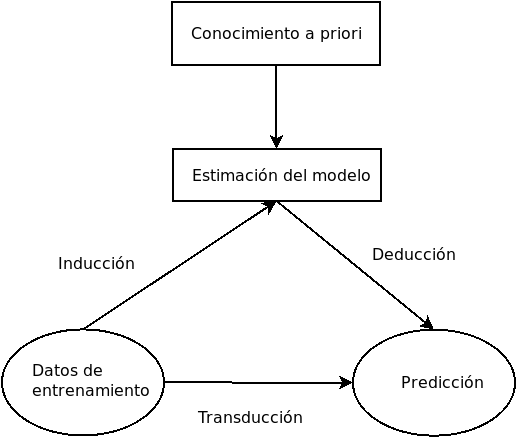
\includegraphics[scale=0.5]{imagenes/induccion_deduccion_transduccion}
	\label{ind_ded_trans}
	\caption{Tipos de inferencia y transduccion \cite[p.~41]{cherkassky_learning_2007}}
\end{figure}

Podemos ver que el conocimiento a priori que tenemos del problema se manifiesta una vez se crea el modelo general, de forma que se emplearía en el paso de la inducción. Ya hemos hablado previamente del conocimiento a priori y cómo incorporarlo al modelo, pero por concretar un poco más podemos añadirlo básicamente de dos formas:

\begin{itemize}
	\item Escogiendo un conjunto de funciones para aproximar la salida del sistema
	\item Añadiendo restricciones o penalizaciones adicionales a dicho conjunto de funciones.
\end{itemize}

En resumen, para poder crear la generalización del modelo de forma única necesitamos:

\begin{enumerate}
	\item Un conjunto de funciones para aproximar la salida.
	\item Conocimiento a priori.
	\item Un principio inductivo, que no es más que una indicación de cómo emplear los datos para llegar a la generalización del modelo.
	\item Un método de aprendizaje, es decir, una implementación del principio inductivo.
\end{enumerate}

En secciones posteriores revisaremos algunos de los principios inductivos más usados pero es importante reseñar la diferencia entre pricipio inductivo y método de aprendizaje. Para un mismo principio inductivo podemos tener varios métodos de aprendizaje, pues podemos escoger diferentes formas de llevarlo a la práctica. Por ejemplo, uno de los principios inductivos más empleados es el ERM o Empirical Risk Minimization, es decir, minimización del error empírico. Podríamos pensar en diferentes formas de utilizar este principio, por ejemplo sólo avanzamos en la creación del modelo si a cada paso que demos minimizamos el error, o por ejemplo vamos avanzando varios modelos a la vez hasta obtener un número de modelos finales de entre los cuales escogeremos aquel que mejor minimice dicho error.

\subsection{Principios inductivos}

Una vez introducido el concepto como hemos hecho en la sección anterior vamos a hacer un breve repaso de los principios más usados y en qué consiste cada uno de ellos.

\subsubsection{Penalización o Regularización}

Imaginemos que tenemos una clase de funciones muy flexible, esto es con un gran número de parámetros libres $f(x,\omega)$ con $\omega \in \Omega$. Vamos a partir de la base del ERM, es decir, minimizar el error empírico. La penalización lo que va a hacer es añadir un factor a la función a minimizar:

$$R_{pen}(\omega) = R_{emp}(\omega) + \lambda \phi [f(x,\omega)]$$

Donde $R_{emp}(\omega)$ es el error empírico con los parámetros $\omega$ y $\phi [f(x,\omega)]$ es un funcional no negativo asociado a cada estimación $f(x,\omega)$. El parámetro $\lambda >0$ es un escalar que controla el peso de la penalización.

El funcional $\phi [f(x,\omega)]$ puede medir lo que creamos conveniente que debemos añadir, es decir, aquí podemos añadir a la minimización algún tipo de medida que nos diga cómo de bien funciona el ajuste de los datos y cómo de bien funciona la información a priori que hemos incluido en el modelo. Pensemos por ejemplo que $\lambda$ fuera un parámetro con un valor muy alto. En este caso la penalización por un mal ajuste de los datos no sería de gran importancia pues lo más conveniente sería minimizar el valor del funcional para no obtener una gran penalización. De esta forma podemos ajustar y dar un poco más de información al error empírico. Por ejemplo, en función del problema, es posible medir la complejidad de la solución mediante el funcional $\phi$ y de esta forma no sólo vamos a obtener una función que ajuste bien los datos, si no que también mantenga una cierta simplicidad para evitar por ejemplo el sobreajuste.

\subsubsection{Reglas de parada anticipada}

Pensemos en un método que vaya aprendiendo de los datos de forma iterativa intentando a cada iteración reducir el error cometido, por ejemplo el ERM. Los métodos o reglas de parada anticipada pueden verse como penalizaciones sobre el algoritmo conforme se va ejecutando. Las reglas de parada anticipada, como su nombre indica lo que preveen es la parada del algoritmo antes de obtener su objetivo teórico. Por ejemplo un algoritmo intenta que el error sea menor que $10^{-6}$ pero para reducirlo desde $10^{-4}$ hasta $10^{-5}$ está consumiendo millones de iteraciones. Si queremos que el tiempo de cómputo penalice lo que podemos hacer es fijar por ejemplo un número máximo de iteraciones que detenga el método aunque no se haya alcanzado esa barrera de error que se preveía.

\subsubsection{Minimización del riesgo estructural o SRM}

Para entender esta filosofía nos ponemos en la situación de que ya sabemos la clase de funciones con la que vamos a aproximar la salida del sistema, por ejemplo hemos escogido la clase de funciones polinómicas. Bajo esta clase de funciones podemos ordenar las funciones por complejidad, entendiendo por complejidad el número de parámetros de la función. Por ejemplo los polinomios de grado $m$ son de menor complejidad que los de grado $m+1$. De esta forma podemos pensar en una estructura de la clase de funciones de la forma:

$$S_0 \subset S_1 \subset S_2 \subset \cdots$$

Este parámetro de complejidad también puede ser un principio a minimizar para intentar conseguir una solución adecuada pero también simple. La generalización de la medida de complejidad para las clases de funciones es la conocida como dimensión VC o dimensión de Vapnik-Chervonenkis.

\subsubsection{Inferencia Bayesiana}

Este principio inductivo se utiliza en el problema de estimación de la función de densidad. El principio es utilizar la conocida fórmula de Bayes para hacer una estimación de la función de densidad empleando el conocimiento a priori que disponemos del problema. La forma en la que se emplea esta fórmula es de la siguiente:

$$P[modelo | datos] = \frac{P[datos | modelo] \cdot P[modelo]}{P[datos]}$$

donde $P[modelo]$ es la probabilidad a priori, $P[datos]$ es la probabilidad de los datos de entrenamiento y $P[datos | modelo]$ es la probabilidad de que los datos estén generados por el modelo.

\subsubsection{Descripción de mínima longitud}

La idea de este principio es la minimización de la longitud que se necesita emplear para describir un modelo y la correspondiente salida. Llamamos l a la longitud total:

$$l = L(modelo) + L(datos | modelo)$$

Esta medida puede ser vista como una medida de complejidad conjunta de todo el modelo.

\section{Regularización}

Por la importancia de este principio inductivo vamos a desarrollarlo un poco más, junto con el concepto de penalización, la selección de los modelos y la relación entre sesgo y varianza. Este último es un concepto muy relevante en cuanto al aprendizaje y que en nuestro caso, al no poseer la clasificación real tendremos que tenerlo en cuenta.

\subsection{Problema de la alta dimensionalidad}

Sabemos que cuando estamos ante un problema de aprendizaje nuestro objetivo es conseguir estimar una función con un número finito de instancias de una muestra ya con la salida. Al tener un número finito de elementos en la muestra ya sabemos que no podemos garantizar que la respuesta sea la óptima o correcta, pero además debemos pensar que a mayor regularidad del conjunto de funciones empleado debemos tener una densidad suficiente de puntos para compensar dicha regularidad. Este problema es conocido como la maldición de la dimensionalidad (curse of dimensionality). El problema es que cuanto mayor sea la dimensionalidad considerada más difícil es poder tener esa alta densidad de datos que se requieren para funciones muy regulares.

Este problema que conlleva la alta dimensionalidad proviene de la geometría de los espacio con alta dimensionalidad. A medida que incrementamos la dimensionalidad el espacio se ve cada vez con más aristas o picos. Podemos pensar en un cubo para el espacio tridimensional y a medida que aumentamos la dimensión incorporamos más aristas y vértices. Podemos resumir en 4 propiedades de los espacio con alta dimensionalidad que causan este problema:

\begin{enumerate}
	\item La densidad disminuye exponencialmente al aumentar el número de dimensiones. Supongamos que tenemos una muestra de $n$ puntos en $\mathbb{R}$. Para poder tener la misma densidad en un espacio $d$-dimensional $\mathbb{R}^d$ necesidamos $n^d$ puntos.
	\item Cuanto mayor dimensionalidad tenga el conjunto de datos mayor lado se necesita para que un hipercubo contenga el mismo porcentaje del conjunto que con una menor dimensionalidad. Imaginemos que tenemos un conjunto $d$-dimensional en el que tenemos la muestra dentro de un hipercubo unidad. Si quisiéramos abarcar un porcentaje $p\in [0,1]$ necesitaríamos un cubo de lado $e_d (p) = p^{\frac{1}{d}}$. Como se puede observar a mayor dimensionalidad y $p$ constante el lado es cada vez mayor. Esta idea es fácilemente entendible si observamos la siguiente figura:
	
	\begin{figure}[H]
		\centering
		\label{radio_alta_dimensionalidad}
		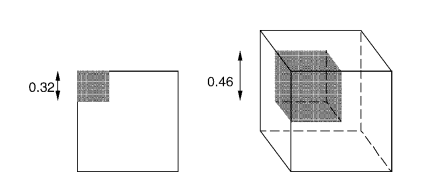
\includegraphics[scale=0.6]{imagenes/radio_alta_dimensionalidad}
		\caption{Para 2 dimensiones necesitamos menor lado que para 3 dimensiones. \cite[p.~64]{cherkassky_learning_2007}}
	\end{figure}
	\item Casi todo punto está más cerca de un borde que de otro punto. Pensemos en un conjunto de datos con $n$ puntos distribuidos de forma uniforme en una bola $d$-dimensional de radio unidad. Para este conjunto de datos, según \cite{hastie_t._elements_nodate}, la distancia media entre el centro de la distribución y los puntos más cercanos a dicho centro se mide bajo la fórmula:
	
	$$D(d,n) = (1-\frac{1}{2}^{1/n})^{1/d}$$
	
	Si en esta fórmula tomamos por ejemplo $n=200$ y $d=10$ el resultado es $D(10,200) \approx 0.57$. Esto significa que los puntos más cercanos al centro de la distribución están más cerca de los bordes que del centro.
	\item Casi todo punto es una anomalía sobre su propia proyección. Si pensamos de nuevo en la idea de los vértices y aristas en espacio de alta dimensionalidad y pensamos en que, según el punto anterior, cada vez que aumenta la dimensionalidad los puntos están más cerca de los bordes entonces no es extraño pensar que los puntos a medida que aumenta la dimensionalidad están más distantes del resto de puntos. Esto intuitivamente (ya que aún no hemos visto la definición formal de anomalía) nos guía a pensar que vistos los puntos en sus propios entornos éstos serán anomalías comparados con el resto.
	
	\begin{figure}[H]
		\centering
		\label{espacio_alta_dimension}
		
\includegraphics[scale=0.6]{imagenes/espacio_alta_dimension}
		\caption{Forma conceptual de un espacio de alta dimensionalidad.\cite[p.~64]{cherkassky_learning_2007}}
	\end{figure}

	Conceptualmente podemos imaginarlo con esta forma de picos, con lo que si tenemos los datos apiñados en dichos picos o extremos el resto de datos que estén en picos diferentes distan tanto del que estamos considerando que no podemos afirmar que tengan ninguna relación entre sí.
\end{enumerate}

Estos puntos hemos de recordar que van referidos al conjunto de datos y no a las funciones que estamos considerando para representar la salida del sistema. Si estamos considerando la complejidad de las funciones la dimensionalidad no es una buena medida. Sabemos de la existencia de teoremas de aproximación de funciones como por ejemplo el Teorema de Superposición de Kolmogorov-Arnold.

\begin{teorema}[Teorema de Superposición de Kolmogorov-Arnold]
	Sea $f$ una función continua de varias variables $f:X_1 \times ... \times X_n \rightarrow \mathbb{R}$, entonces existen funciones $\Phi_q : \mathbb{R}\rightarrow \mathbb{R}$ y $\phi_{q,p} : X_p \rightarrow [0,1]$ tales que $f$ se puede expresar como:
	
	$$f(x) = f(x_1, ..., x_n) = \sum_{q=0}^{2n}\Phi_q ( \sum_{p=1}^{n}\phi_{q,p}(x_p))$$
\end{teorema}

Este Teorema argumenta perfectamente que la complejidad que le damos a los datos por tener una alta dimensionalidad no es transferible a las funciones pues podemos expresar funciones de varias variables como combinación de funciones de una sola variables. En otras palabras no podemos argumentar que la complejidad de funciones univariantes sea mayor o menor que la de funciones multivariantes.

\subsection{Aproximación de funciones}

Como ya hemos dicho en la introducción queremos aproximar una función salida del sistema dentro de una familia de funciones. Este campo no es nuevo, tenemos como herramientas una serie de Teoremas relacionados con la aproximación de funciones como el Teorema de Kolmogorov enunciado anteriormente o el Teorema de aproximación de Weierstrass.

La versión más simple del Teorema de Weierstrass es la de funciones reales definidas en intervalos cerrados, veamos un repaso de estos Teoremas para hacer un esquema de la aproximación de funciones.

\begin{teorema}[Teorema de aproximación de Weierstrass]
	Supongamos que $f:[a,b] \rightarrow \mathbb{R}$ es una función continua. Entonces $\forall \epsilon >0$, $\exists p$ un polinomio tal que $\forall x\in [a,b]$ tenemos que $|f(x)-p(x)|<\epsilon$.
\end{teorema}

En otras palabras, podemos aproximar las funciones continuas reales definidas en un intervalo cerrado con el error que queramos en un punto mediante polinomios. Además tenemos versiones más generales aún como el Teorema de Stone-Weierstrass para funciones reales, para espacios localmente compactos y para el espacio de los complejos.

Estas aproximaciones son más sencillas en términos de la complejidad de la clase de funciones, pero tenemos aproximaciones muy famosas, como por ejemplo la serie de Fourier.

\begin{definicion}[Serie de Fourier]
	Si tenemos una función $f:\mathbb{R} \rightarrow \mathbb{R}$ integrable en el intervalo $[t_0 - \frac{T}{2}, t_0 + \frac{T}{2}]$ entonces se puede obtener el desarrollo en serie de Fourier de $f$ en dicho intervalo. Si $f$ es periódica en toda la recta real la aproximación será válida en todos los valores en los que esté definida.
	
	$$f(t) \approx \frac{a_0}{2} + \sum_{n=1}^{\infty}[a_n \cos (\frac{2n\pi}{T}t) + b_n\sin (\frac{2n\pi}{T}t)]$$
	
	Donde $a_0, a_n$ y $b_n$ son los coeficientes de la serie de Fourier que tienen la forma:
	
	$$a_0 = \frac{2}{T}\int_{-\frac{T}{2}}^{\frac{T}{2}}f(t)dt$$
	
	$$a_n = \frac{2}{T}\int_{-\frac{T}{2}}^{\frac{T}{2}}f(t) cos(\frac{2n\pi}{T}t)dt$$
	
	$$b_n = \frac{2}{T}\int_{-\frac{T}{2}}^{\frac{T}{2}}f(t) \sin (\frac{2n\pi}{T}t)dt$$
\end{definicion}

Como podemos ver hemos introducido dos conocidas formas de aproximar funciones, una con funciones polinómicas y otra con funciones trigonométricas. Vamos a dividir en dos los tipos de  aproximación que podemos tener para el problema de aprendizaje.

\begin{enumerate}
	\item Aproximaciones universales: son aquellas en las que se establece que cualquier función continua puede ser aproximada por otra función de otra clase con el error que queramos. En este grupo podríamos meter a los dos teoremas que hemos dado previamente. Dentro de este grupo podemos tener diferentes tipos de aproximaciones en función de la familia de funciones que escojamos como aproximaciones. Por ejemplo en los dos teoremas previos hemos cogido las clases de funciones polinómicas y trigonométricas pero podríamos haber tomado otras clases diferentes.
	\item Aproximaciones inexactas: son aquellas en las que no podemos tener una aproximación como las que hemos dado en los teoremas previos, si no que proveen de una aproximación de peor calidad.
\end{enumerate}

\subsection{Penalización o control de la complejidad}

Ya hemos discutido brevemente en la sección de principios inductivos la complejidad y cómo penalizarla. Vamos a ver qué elementos queremos controlar con la penalización:

\begin{enumerate}
	\item La clase de funciones con la que vamos a hacer la aproximación. Tenemos que decidir si escoger una clase tan amplia que nos aseguremos que abarque la solución seguro pero penalicemos la complejidad de la elección o queremos una clase de funciones más ajustada.
	\item Tipo de funcional de penalización. Tenemos que escoger entre los distintos tipos de penalización que queremos. Esto se reduce a escoger entre dos tipos de penalización: paramétrica y no paramétrica. La primera de ellas se basa en estudiar la suavidad del ajuste junto con el número de parámetros que requiere la aproximación mientras que la segunda intenta estudiar lo mismo, es decir la suavidad del ajuste, sin medir los parámetros de la clase de funciones. En este punto se puede incorporar el conocimiento a priori del problema.
	\item Método con el que queremos minimizar la penalización. Este apartado está relacionado con los métodos que tenemos de aprender de los datos y el objetivo será intentar hallar una forma eficiente de minimizar tanto el error de la aproximación como la propia penalización.
	\item Control de la complejidad. Como hemos dicho antes el control de la complejidad no es algo sencillo y habrá que escoger la mejor manera de medir dicha complejidad. En secciones posteriores veremos medidas de complejidad como la dimensión de Vapnik-Chervonenkis.
\end{enumerate}

Veamos brevemente la distinción que hemos hecho entre la penalización paramétrica y no paramétrica.

\subsubsection{Penalización paramétrica}

Supongamos que tenemos un conjunto de funciones $f(x,\omega)$ con $\omega \in \Omega$ donde $\Omega$ es el conjunto de parámetros de la forma $\omega = (\omega_0 , ... , \omega_m)$. Como la aproximación viene definida por el parámetros $\omega$ entonces podemos definir también la penalización asociada a dicha selección de parámetros.

Vamos a ver los ejemplos de las penalizaciones más empleadas de este tipo.

\begin{itemize}
	\item Ridge: $\phi_r (\omega_m) = \sum_{i=0}^{m}\omega_i^2$
	\item Selección de subconjunto: $\phi_s (\omega_m) = \sum_{i=0}^{m}\chi (\omega_i \neq 0)$
	\item Bridge: $\phi_p (\omega_m) = \sum_{i=0}^{m}|\omega_i|^p$
	\item Decaimiento de peso: $\phi_q (\omega_m) = \sum_{i=0}^{m}\frac{(\omega_i / q)^2}{1+(\omega_i / q)^2}$ 
\end{itemize}

\subsubsection{Penalización no paramétrica}

En primer lugar vamos a definir la transformada de Fourier de una función para poder definir el funcional de penalización. 

\begin{definicion}[Transformada de Fourier]
	Sea $f$ una función integrable Lebesgue, $f\in L(\mathbb{R})$. Se define la transformada de Fourier de $f$ como la función:
	
	$$\mathcal{F}\{f\} : \xi \rightarrow \hat{f}(\xi) := \int_{-\infty}^{\infty}f(x)e^{-2\pi i\xi x}dx$$
\end{definicion}

Recordemos brevemente las propiedades de la transformada de Fourier.

\begin{itemize}
	\item La transformada de Fourier es un operador lineal: $\mathcal{F}\{a\cdot f + b\cdot g\} = a\mathcal{F}\{f\} + b\cdot \mathcal{F}\{g\}$
	\item $\mathcal{F}\{f(at)\}(\xi) = \frac{1}{|a|}\cdot \mathcal{F}\{f\}(\frac{\xi}{a})$
	\item $\mathcal{F}\{f(t-a)\}(\xi) = e^{-\pi i\xi a}\cdot \mathcal{F}\{f\}(\xi)$
	\item $\mathcal{F}\{f\}(\xi -a) = \mathcal{F}\{e^{\pi iat}f(t)\}(\xi)$
	\item $\mathcal{F}\{f'\}(\xi) = 2\pi i\xi \mathcal{F}\{f\}(\xi)$
	\item $\mathcal{F}\{f\}'(\xi) = \mathcal{F}\{(-it)\cdot f(t)\}(\xi)$
\end{itemize}

Habiendo recordado esto podemos definir el funcional de penalización no paramétrica. Este funcional mide la suavidad del ajuste de la función gracias a que se puede medir, mediante la transformada de Fourier, la ondulación de la función. Por tanto el funcional no paramétrico que se propone es:

$$\phi [f] = \int_{\mathbb{R}^d}\frac{|\hat{f}(s)|^2}{\hat{G}(s)}ds$$

Donde $\hat{f}$ indica la transformada de Fourier de la función $f$ y $\frac{1}{\hat{G}}$ es la transformada de Fourier de una función de filtro de paso alto. Es en esta proposición de filtro donde se añade el conocimiento a priori del problema. Por ejemplo pudiera ser interesante en alguna aplicación práctica tener un funcional invariante frente a rotaciones de funciones.

\subsection{Equilibrio entre el sesgo y la varianza}

Este enfoque es muy utilizado en el estudio del error, dividiéndolo en sesgo y varianza para hacer un mejor estudio del mismo y poder enfrentar ambos con varios métodos. Este estudio del caso clásico no es válido (o al menos no del todo) para problemas no supervisados como es nuestro caso. Vamos a hacer una adaptación de esta teoría para que pueda encajar en nuestro caso de estudio.

Tenemos que tener en cuenta que no conocemos la salida real del sistema en el caso de detección de anomalías, es decir, no sabemos estimar con certeza el sesgo y la varianza y por tanto el error que cometemos. En primer lugar vamos a ver una pequeña adaptación de la notación al caso de detección de anomalías para poder hacer un estudio enfocado.

Vamos a notar por $X_1 , ... , X_n$ los datos de test y $\mathcal{D}$ como conjunto de datos de entrenamiento. Además vamos a considerar que existe una función $f$ que nos da la etiqueta real de un dato, esto es, si es o no una anomalía. Por tanto podemos decir que la auténtica etiqueda de un dato es $y_i = f(X_i)$. Además nosotros estaremos usando un modelo ya escogido por nosotros para predecir la etiqueta de un dato de test, esto es $g(X_i, \mathcal{D})\approx y_i+\beta$ donde $\beta$ es un cierto error.

Una vez conocida esta notación podemos definir el error medio al cuadrado como:

$$MSE = \frac{1}{n}\sum_{i=1}^{n}\{y_i - g(X_i, \mathcal{D})\}^2$$

Y podemos definir también el valor esperado del error medio al cuadrado como:

$$E[MSE] = \frac{1}{n} \sum_{i=1}^{n}E[\{y_i - g(X_i, \mathcal{D}\}^2]$$

Una vez definido el $MSE$ esperado podemos desarrollar un poco el cálculo para poder obtener el error y la varianza que esperamos.

En primer lugar podemos escribirlo como:

$$E[MSE] = \frac{1}{n}\sum_{i=1}^{n}E[\{ (y_i-f(X_i)) + (f(X_i) - g(X_i,\mathcal{D})) \}^2]$$

Aquí solo hemos restado y sumado $f(X_i)$, ahora si recordamos que $y_i = f(X_i)$ entonces podemos igualar el primero de los paréntesis a $0$ y por tanto nos queda:

$$E[MSE] = \frac{1}{n}\sum_{i=1}^{n}E[\{ f(X_i) - g(X_i, \mathcal{D}) \}^2]$$

Si seguimos descomponiendo podemos sumar y restar $E[g(X_i, \mathcal{D})]$ con lo que nos quedaría:

$$E[MSE] = \frac{1}{n}\sum_{i=1}^{n}E[\{ f(X_i) - E[g(X_i, \mathcal{D})] \}^2]$$

$$ + \frac{2}{n}\sum_{i=1}^{n}\{ f(X_i) - E[g(X_i, \mathcal{D})] \}\cdot \{ E[g(X_i, \mathcal{D})] - E[g(X_i, \mathcal{D})] \}$$

$$ + \frac{1}{n}E[\{ E[g(X_i, \mathcal{D}) - g(X_i, \mathcal{D})] \}^2]$$

Como es claro, el segundo término da cero por lo que nos queda al final:

$$E[MSE] = \frac{1}{n} \sum_{i=1}^{n}E[\{ f(X_i) - E[g(X_i, \mathcal{D})] \}^2] + \frac{1}{n}\sum_{i=1}^{n}E[\{ E[g(X_i, \mathcal{D})] - g(X_i, \mathcal{D}) \}^2]$$

$$=\frac{1}{n}\sum_{i=1}^{n}\{ f(X_i) - E[g(X_i, \mathcal{D})] \}^2 + \frac{1}{n}\sum_{i=1}^{n}E[\{ E[g(X_i, \mathcal{D})] - g(X_i, \mathcal{D}) \}^2]$$

Si reconocemos cada uno de los términos, en primer lugar el primero de ellos es el sesgo al cuadrado y el segundo la varianza, por lo que finalmente lo que hemos obtenido es:

$$E[MSE] = sesgo^2 + varianza$$

El dilema que se nos plantea es el siguiente: si tomamos modelos con un bajo sesgo en la estimación de los parámetros entonces tendremos una alta varianza y viceversa. Esto significa que no podemos con el conocimiento del que disponemos disminuir tanto el sesgo como la varianza a la vez. Es esta propiedad la que se conoce como la compensación entre sesgo y varianza.

\section{Teoría estadística del aprendizaje}

En esta sección vamos a hacer un repaso por la teoría del aprendizaje, en concreto la teoría desarrollada por Vapnik-Chervonenkis. Esta teoría se basa o tiene como pilares cuatro puntos:

\begin{enumerate}
	\item Condiciones para la consistencia del principio ERM o minimización del error empírico.
	\item Cotas en la capacidad de generalización de las máquinas de aprendizaje.
	\item Principios de inferencia sobre muestras finitas.
	\item Métodos constructivos para implementar los principios inductivos ya expuestos.
\end{enumerate}

Durante el desarrollo de esta sección haremos un repaso de estos cuatro puntos para dar el broche final a esta sección y poder realizar la primera de las definiciones de anomalía.

\subsection{Condiciones para la convergencia y consistencia del ERM}

En el problema de aprendizaje disponemos de una muestra en la que tenemos los propios datos de entrada y la salida del sistema. Denotemos a estos elementos por $z=(x,y)$ donde $x$ son los datos de entrada e $y$ la salida del sistema. Por tanto la muestra que se nos da es un conjunto $Z_n = \{ z_1 , ... , z_n \}$. Estos datos están generados como ya sabemos mediante una función de densidad desconocida $p(z)$. Sobre este esquema tenemos una serie de funciones de pérdida y un funcional de pérdida. El objetivo es encontrar dicha función de pérdida $Q(z,\omega )$ que minimice dicho funcional:

$$R(\omega) = \int Q(z,\omega) p(z)dz$$

Por tanto si tenemos la función de pérdida podemos definir el error empírico como:

$$R_{emp}(\omega) = \sum_{i=1}^{n}Q(z_i, \omega)$$

Donde $\omega$ son los parámetros escogidos para el modelo.

Para poder estudiar la consistencia del ERM primero debemos definir formalmente dicha propiedad. Denotamos por $R_{emp}(\omega_n^*)$ el valor del error empírico con la función de pérdida $Q(z,\omega_n^*)$ que minimiza el error empírico para el conjunto de entrenamiento $Z_n$. Denotemos además por $R(\omega_n^*)$ el verdadero valor (desconocido) del error para la función de pérdida. Como se puede ver estos valores dependen del tamaño del conjunto de entrenamiento $n$, podemos por tanto estudiar cómo se comportan estos errores cuando aumentamos el tamaño del conjunto de entrenamiento. Es aquí donde entra la definición de consistencia del ERM. Decimos que es consistente si la sucesión de errores reales y empíricos convergen en probabilidad al mismo límite $R(\omega_0) = \min_{\omega} R(\omega)$. Es decir:

$$R(\omega_n^*) \rightarrow R(\omega_0) \ cuando \ n\rightarrow \infty$$
$$R_{emp}(\omega_n^*) \rightarrow R(\omega_0) \ cuando \ n\rightarrow \infty$$

Para poder asegurar esta propiedad sobre el ERM tenemos el conocido como Teorema Clave de la Teoría del Aprendizaje de Vapnik y Chervonenkis.

\begin{teorema}[Teorema Clave de la Teoría del Aprendizaje]
	Para funciones de pérdida acotadas el principio inductivo de minimización del error empírico es consistente sí y sólo si el error empírico converge uniformemente al valor real del error en el siguiente sentido:
	
	$$\lim\limits_{n\rightarrow \infty} P[\sup_{\omega}|R(\omega) - R_{emp}(\omega)|>\epsilon] = 0 \ , \ \forall \epsilon >0$$
\end{teorema}

Cabe recalcar que estas condiciones de consistencia dependen de las propiedades de la clase de funciones elegida. No podemos pretender escoger como clase de aproximación una muy general y seguir manteniendo las condiciones de consistencia del ERM. Aún así el teorema nos está dando condiciones generales para la consistencia del ERM pero son abstractas y no fácilmente aplicables en la práctica. Para ello vamos a estudiar las condiciones de convergencia de ERM que sí serán aplicables en la implementación de algoritmos.

Vamos ahora a particularizar el estudio en el caso de clasificación binaria por ser la materia de estudio que nos ocupa, pues al final tendremos que clasificar instancias en anómalas o no anómalas. Ahora las funciones de pérdida $Q(z,\omega)$ son funciones de pérdida indicadoras. Vamos a notar por $N(Z_n)$ el número de dicotomías que se pueden tener con la clase de funciones elegidas. Esto es el número de formas de clasificar los datos en las dos clases existentes.

Una vez actualizada nuestra notación podemos definir la entropía aleatoria como $H(Z_n) = \ln N(Z_n)$. Esta cantidad es una variable aleatoria dependiente de los valores de entenamiento $Z_n$, podemos definir ahora la entropía de Vapnik-Chervonenkis como el valor medio o esperado de la entropía aleatoria:

$$H(n) = E[\ln N(Z_n)]$$

Esta medida es una cuantificación de la diversidad del conjunto de funciones indicadoras que nos pueden separar los datos en ambas clases.

Por último vamos a definir la función de crecimiento que nos va a permitir hacer cotas y llegar a la condición necesaria y suficiente para la convergencia del ERM. Definimos la función de crecimiento como:

$$G(n) = \ln \max_{Z_n} N(Z_n)$$

Donde aquí estamos notando el máximo número de dicotomías sobre todas las posibles muestras existentes de tamaño $n$. Es más, como el máximo número de formas de dividir un conjunto de tamaño $n$ en dos clases es $2^n$ entonces podemos afirmar que $G(n)\leq n\ln (2)$.

Por último y para completar la cadena de desigualdades que buscamos vamos a definir la entropía reforzada de Vapnik-Chervonenkis:

$$H_{ann}(n) = \ln (E[N(Z_n)])$$

Haciendo uso de la conocida desigualdad de Jensen

$$\sum_{i=1}^{n}a_i \ln (x_i) \leq \ln (\sum_{i=1}^{n}a_i x_i)$$

podemos ver claramente que $H(n)\leq H_{ann}(n)$. Por tanto obtenemos la cadena de desigualdades:

$$H(n)\leq H_{ann}(n) \leq G(n) \leq n\ln (2)$$

La condición necesaria y suficiente de Vapnik-Chervonenkis para la convergencia del ERM que hallaron fue que:

$$\lim\limits_{n\rightarrow \infty} \frac{H(n)}{n} = 0$$

Pero esta condición no asegura una convergencia rápida asintóticamente al error real. Se dice que el ratio de convergencia es rápido asintóticamente en la Teoría de Vapkin-Chervonenkis si:

$$\forall n>n_0 \ P(R(\omega) - R(\omega^*)<\epsilon) = e^{-cn\epsilon^2} \ con \ c>0$$

Para poder cumplir esta condición se dio la condición suficiente para la convergencia rápida:

$$\lim\limits_{n\rightarrow \infty} \frac{H_{ann}(n)}{n} = 0$$

Estas condiciones son dependientes de la distribución de los datos $Z_n$ como es claro al depender de la esperanza de una variable aleatoria dependiente de $Z_n$. Es por tanto que esta condición no es del todo general. Para solventar esto se tiene la consistencia y convergencia del ERM con la condición necesaria y suficiente de que:

$$\lim\limits_{n\rightarrow \infty}\frac{G(n)}{n}$$

Por tanto este estudio nos ha dado las condiciones de convergencia y consistencia del ERM.

\chapter{Concepto de anomalía}
\label{chapter:anomalia}
%
\chapter{Concepto de anomalía}
\label{chapter:anomalia}

\section{Contextualización}

Ya hemos discutido previamente una idea intuitiva del concepto de anomalía. Un dato decimos que es anómalo cuando se distancia del resto de los datos lo suficiente como para no tener características comunes con ellos.

Este hecho puede ser por distintos motivos. Puede que la anomalía venga del hecho de que se está produciendo un evento en nuestros experimentos que no sea nada frecuente. Por ejemplo podemos estar midiendo datos meteorológicos y que en un momento dado se den una serie de fenómenos que no sea frecuente ver juntos, o incluso que no se hayan visto nunca ocurrir simultáneamente. Otra forma de tener una anomalía en nuestro conjunto de datos pudiera ser errores de medición. Por ejemplo si seguimos con este símil de los datos meteorológicos imaginemos que nuestra estación dispone de un termómetro. Este sensor se ha roto y empieza a marcar datos superiores a 100 $C^\circ$, claramente son datos muy desviados de las temperaturas normales con lo que no tendrían relación con el resto y presentaría una desviación muy importante con respecto al resto de los datos.

\section{Criterios}

Esta idea intuitiva que estamos dando de anomalía no refleja todos los posibles escenarios. Los ejemplos que estamos dando suponen una desviación muy grande de los datos normales, tanto que no se pueden comparar con el resto porque difieren mucho numéricamente. Vamos a plantear un escenario para dar una mejor forma al concepto de anomalía. Pensemos en una serie de datos muy agrupados en dos clústeres por ejemplo:

\begin{figure}[H]
	\centering
	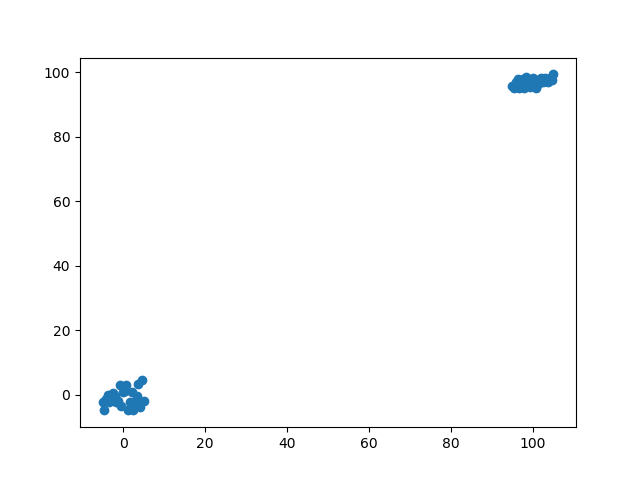
\includegraphics[scale=0.5]{imagenes/clusters}
	\label{clusters}
	\caption{Clústeres alejados}
\end{figure}

Como podemos comprobar que tenemos dos clústeres no sólo alejados entre sí, si no con los elementos muy concentrados para poner un caso extremo. Ahora no vamos a proponer un valor que se aleje de los dos clústeres, si no uno que esté a medio camino entre los dos:

\begin{figure}[H]
	\centering
	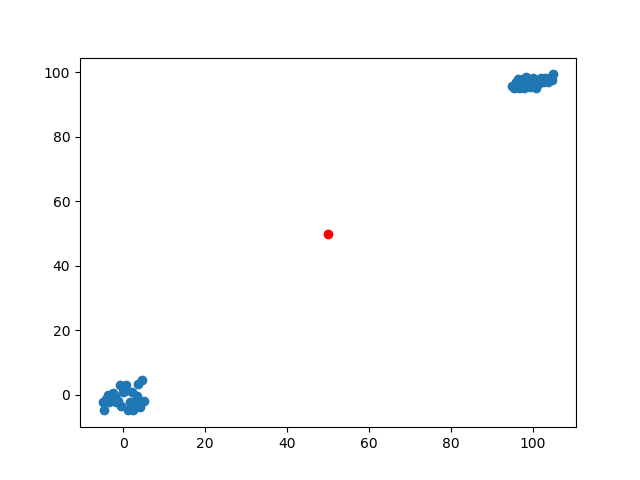
\includegraphics[scale=0.5]{imagenes/outlier_cluster}
	\label{outlier_clusters}
	\caption{Clústeres alejados con una anomalía en rojo}
\end{figure}

Si los datos del clúster de abajo a la izquierda fueran datos de temperatura con valores entorno a 0 y los de arriba a la derecha fueran de datos de temperatura entorno a 100 grados nuestro datos anómalo tendría una temperatura de unos 50 grados. Esta temperatura no se aleja radicalmente de los valores normales, es decir, no son -1000 grados ni 1000 grados. Aún así estamos describiendo una situación anómala.

No podemos dar una definición formal o que podamos decir que abarca todos los casos para definir lo que es una anomalía, aún así vamos a intentar dar dos puntos de vista: uno basado en distancias y otro en probabilidades.

El criterio más usado en la definición o detección de anomalías es el llamado ``Tukey's Fences''. Para introducirlo vamos a ver su definición en una única dimensión para luego extender el concepto. Pensemos en un conjunto de datos 1-D. Sobre sus valores podemos calcular los cuartiles $Q_1 , Q_2 $ y $Q_3$. Un valor anómalo es aquel que no cae dentro del intervalo $[Q_1 - k(Q_3 - Q_1), Q_3 + k(Q_3 - Q_1)]$ donde $k$ es una constante. El valor propuesto para $k$ por Tukey fue de $k=1.5$ aunque algunos autores más restrictivos proponen $k=3$.

Este criterio puede ser extendido al caso de mayor dimensionalidad si realizamos este mismo test sobre todos los valores de todas las características y comprobar si alguno o todos se salen del rango en función de cómo de restrictivo queremos que sea el criterio.

Esta extensión es muy vaga, por lo que se propone un criterio un poco más fijado. Imaginemos los datos agrupados por clústeres, entonces podemos fijar un centroide de dicho clúster. Sobre cada clúster podemos medir cuál es la mayor distancia dentro del clúster de los datos al centroide. Podemos extender el criterio de Tukey diciendo que un dato anómalo es aquel que se distancia más de $1.5$ veces de la mayor distancia dentro del clúster al centroide.

Esta generalización ya si abarca el ejemplo que hemos propuesto. Al estar muy apiñados los datos entorno al centroide la mayor distancia dentro del clúster es muy pequeña, de hecho en el ejemplo construido es menor que 5. Por tanto el dato $(50,50)$ está alejado más de $1.5 \cdot 5 = 7.5$ unidades del centroide y por tanto lo podemos considerar una anomalía.

\section{Qué hacer con las anomalías}

Estamos estudiando cómo podemos detectar anomalías pero una vez que las hayamos detectado en nuestros conjuntos de datos en un problema real, ¿qué debemos hacer con ellas? Este problema es algo muy general, puede que estemos seguros en nuestro caso de que las anomalías se han debido a un problema de medición porque nuestros instrumentos estaban rotos y por tanto deberíamos descartarlos. Puede que sean datos reales pero estén tan separados del resto que debamos estudiarlos de forma separada. Vamos a dar unas cuantas alternativas a lo que podemos hacer una vez que hemos detectados las anomalías dentro de nuestro conjunto de datos:

\begin{itemize}
	\item Dejarlos: puede que nuestro conjunto de datos tenga un número de datos muy elevado y por tanto aparezcan en él anomalías. Estas anomalías no deben ser eliminadas, es más debemos escoger modelos que aprendan o utilicen los datos teniendo en cuenta estas anomalías y siendo robustos ante su aparición.
	\item Exclusión: una opción es eliminar directamente las anomalías. Esto en general no está justificado y de hecho no se recomienda pues perdemos riqueza del conjunto de datos al eliminar instancias del mismo. Aún así, si decidimos eliminar los datos tenemos dos formas de hacerlo. Podemos eliminarlos directamente y prescindir de esos datos o podemos sustituirlos por datos cercanos que no sean anómalos.
	\item Estudiarlos por separado: puede que tengamos un número suficientemente elevado de las mismas y que enseñen algunos patrones o tengan explicación en nuestro ejemplo del mundo real. En este caso quizás deberíamos considerarlas y estudiarlas a parte para darles un sentido y emplear el conocimiento que les subyace.
\end{itemize}
%
\chapter{Introducción de Estadística Multivariante}
\label{chapter:estadistica_multivariante}

Vamos a dar otra definición de anomalía que no coincide con la que hemos visto basada en distancias, pero antes de dar esa definición debemos hacer un breve repaso de estadística multivariante y probabilidad para poder comprender y enmarcar dicha definición.

\section{Introducción}

En primer lugar vamos a describir conceptos básicos sobre los que poder construir los conceptos que necesitamos para la definición de anomalía basada en probabilidades.

En primer lugar vamos a definir el concepto de variable aleatoria.

\begin{definicion}
	Una variable aleatoria es una función $X:\Omega \rightarrow E$ que parte de un espacio de probabilidad $(\Omega , \mathcal{F}, \mathcal{P})$ y llega a un espacio medible $(E, \mathcal{B})$, donde $X$ además es una función medible.
\end{definicion}

Normalmente ya sabemos que $E\subseteq \mathbb{R}$ y además cabe recordar que $\mathcal{F}$ es una $\sigma$-álgebra. Además cabe recordar la definición de función medible:

\begin{definicion}
	Decimos que una función $X: (\Omega , \mathcal{F}, \mathcal{P}) \rightarrow (E, \mathcal{B})$ es medible si $X^{-1}(B)\subset \mathcal{F}$, $\forall B \in \mathcal{B}$.
\end{definicion}

Esta definición puede extenderse al caso vectorial, introduciendo con esto la noción de vector aleatorio:

\begin{definicion}
	Un vector aleatorio $\underline{X} = (X_1 , ... , X_p)$ es una aplicación medible $\underline{X}: (\Omega , \mathcal{F}, \mathcal{P})\rightarrow (E, \mathcal{B}^p)$ donde $E\subseteq \mathbb{R}^p$.
\end{definicion}

Se puede demostrar además la caracterización:

\begin{proposicion}
	Un vector $\underline{X} = (X_1, ..., X_p)$ es un vector aleatorio si y sólo si $X_i : (\Omega , \mathcal{F}, \mathcal{P}) \rightarrow (\mathbb{R}, \mathcal{B})$ es una función medible.
\end{proposicion}

Con este vector aleatorio podemos estudiar o definir la distribución de probabilidad del mismo sobre $( \mathbb{R}^p , \mathcal{B}^p )$ $P_{\underline{X}}$ como:

$$P_{\underline{X}} [B]:= P[\underline{X}^{-1}(B)] \ \forall B\in \mathcal{B}$$

con lo que el espacio $(\mathbb{R}^p , \mathcal{B}^p , P_{\underline{X}})$ es un espacio de probabilidad o probabilístico.

Sobre los conocimientos de la definición de la función de distribución univariante podemos hacer una definición análoga para el caso multivariante.

\begin{definicion}
	Se define la función de distribución asociada a la probabilidad inducida como:
	
	$$F_{\underline{X}} (\underline{x}) = P_{\underline{X}} [X_1 \leq x_1 , ... , X_p \leq x_p] \ , \ \forall \underline{x} = (x_1 , ... , x_p) \in \mathbb{R}^p$$
\end{definicion}

De igual forma podemos caracterizar la función de densidad como aquella $f_{\underline{X}}$ que, de existir, cumple que:

$$F_{\underline{X}} (\underline{x}) = \int_{- \infty}^{x_1} \int_{-\infty}^{x_2} ... \int_{-\infty}^{x_p} f_{\underline{X}}(u_1 , ... , u_p) du_1 ... du_p$$

Otra forma de determinar de forma única la distribución de un vector aleatorio es mediante la función característica, lo que nos va a dar además una caracterización de la independencia que introduciremos en siguiente lugar.

\begin{definicion}
	Dado un vector aleatorio $X = (X_1 , ... , X_p)$ se define la función característica como $\Phi_{\underline{X}} (\underline{t}) = E[e^{i\underline{t}X}]$ con $\underline{t} = (t_1 , ... , t_p)\in \mathbb{R}^p$ donde la función $E[\cdot]$ denota la esperanza, por lo que:
	$$\Phi_{\underline{X}} (\underline{t}) = \int_{\mathbb{R}^p} e^{i\underline{t} \underline{X}} P_{\underline{X}}(d\underline{x})$$
\end{definicion}

Con esto ya podemos introducir el concepto de independencia en varias variables. 

\subsection{Independencia}

\begin{definicion}
	Dados dos vectores aleatorios $\underline{X} = (X_1 , ... , X_p)$, $\underline{Y} = (Y_1 , ... , Y_p)$ se dice que son independientes si:
	$$F_{\underline{X}, \underline{Y}}(\underline{x}, \underline{y}) = F_{\underline{X}}(\underline{x}) \cdot F_{\underline{Y}}(\underline{y})$$
\end{definicion}

Podemos también definir la independencia entre las variables de un vector aleatorio como:

\begin{definicion}
	$X = (X_1 , ... , X_p)$ se dice que está compuesto de variables independientes si $\forall B = B_1 \times ... \times B_p$ con $B_i \in \mathcal{B}$ se tiene que:
	
	$$P_{\underline{X}}(B) = P_{X_1}[B_1] \cdot ... \cdot P_{X_p}[B_p]$$
\end{definicion}

En cuanto a la independencia de sucesos podemos dar dos definiciones de independencia:

\begin{definicion}
	Decimos que los eventos $B = (B_1 , ... , B_p)$ son independientes dos a dos si para todos $m\neq k$ se tiene que $P(B_m \bigcap B_k) = P(B_m)P(B_k)$
\end{definicion}

\begin{definicion}
	Se dice que los eventos $B = (B_1 , ... , B_p)$ son independientes mutuamente si para todo $k\leq p$ se tiene que $P(\bigcap_{i=1}^{k}B_i) = \prod_{i=1}^{k}(B_i)$
\end{definicion}

En cuanto a la definición de independencia entre las variables aleatorias que definen un vector aleatorio podemos dar dos caracterizaciones basadas en la función característica.

\begin{proposicion}
	Si las componentes del vector aleatorio $X = (X_1 , ... , X_p)$ son independientes entonces:
	
	$$\Phi_{\underline{X}}(\underline{t}) = E[e^{i\underline{t}\underline{X}}] = \prod_{j=1}^{p}E[e^{it_j X_j}]$$
\end{proposicion}

\begin{proposicion}
	Si las componentes del vector aleatorio $X = (X_1 , ... , X_p)$ son independientes entonces la función característica de la variable $Y = \sum_{j=1}^{p}X_j$ es:
	
	$$\Phi_Y (t) = E[e^{itY}] = E[e^{it \sum_{j=1}^{p}X_j}] = \prod_{j=1}^{p}\Phi_{X_j} (t)$$
\end{proposicion}

\subsection{Probabilidad y esperanza condicionada}

En esta sección vamos a describir la probabilidad y esperanza condicionada de una variable aleatoria y no de un vector aleatorio. Este hecho es sencillo de deducir, pues como hemos introducido previamente la distribución de probabilidad de un vector aleatorio viene determinada por una distribución de probabilidad de una variable aleatoria. Por tanto el estudio de la probabilidad y esperanza condicionada en el caso univariante se hace válido para el caso multivariante. 

En primer lugar debemos introducir el concepto de probabilidad condicionada tal y cómo la conocemos hasta ahora de Bayes. Partimos de un espacio de probabilidad $(\Omega , \mathcal{A}, \mathcal{P})$.

\begin{definicion}
	Definimos la probabilidad condicionada a un suceso $B\in \mathcal{A}$ con $P(B)>0$ como:
	
	$$P(\cdot | B) : \mathcal{A} \rightarrow [0,1] , \ \ \ P(A | B) = \frac{P(A\cap B)}{P(B)}$$
\end{definicion}

Esta es una función de probabilidad, por lo que nos lleva a pensar en el espacio de probabilidad que genera, es más podemos pensar en el espacio de probabilidad en el que la probabilidad condicionada no se anula, es decir:

$$\mathcal{A}_B = \{ C = A\cap B, \ A\in \mathcal{A} \}$$

Por tanto solemos considerar como espacio de probabilidad condicionada al espacio $(B, \mathcal{A}_B , P(\cdot | B))$.

Partiendo de este espacio de probabilidad podemos considerar una variable aleatoria $X : (\Omega , \mathcal{A}, \mathcal{P}(\cdot | B)) \rightarrow (\mathbb{R}, \mathcal{B})$. 

\begin{definicion}
	Definimos la esperanza de esta variable aleatoria condicionada a $B$ como:
	$$E[X | B] = \int_{\Omega}XdP(\cdot | B) = \int_{\Omega}XdP(\cdot | B) = \frac{1}{P(B)}\int_{B}XdP = \frac{E[X1_B]}{P(B)}$$
	Donde $1_B$ representa la función indicadora del conjunto $B$.
\end{definicion}

No sólo podemos estudiar la probabilidad y esperanzas condicionadas a un evento, si no que también las podemos estudiar condicionadas a una $\sigma$-álgebra. En este terreno vamos a distinguir dos posibilidades: condicionamiento a una $\sigma$-álgebra generada por una partición numerable de sucesos de probabilidad no nula y condicionamiento a una $\sigma$-álgebra arbitraria.

\begin{definicion}
	Definimos la esperanza condicionada a una $\sigma$-álgebra $\mathcal{A}$ generada por $\{ B_n \}\subset \mathcal{A}$ con $B_i \cap B_j = \phi , \ i\neq j$, $\bigcup_{n=1}^{\infty} B_n = \Omega$ y $P(B_i)>0 , \ \forall i$. Siendo la $\mathcal{U} = \sigma (\{ B_n \})$ la $\sigma$-álgebra generada por $\{ B_n \}$. Con este marco, definimos la esperanza de una variable aleatoria $X: (\Omega , \mathcal{A}, P) \rightarrow (\mathbb{R}, \mathcal{B})$ condicionada a la $\sigma$-álgebra $\mathcal{U}$ como:
	
	$$E[X | \mathcal{U}](\omega) = \sum_{n=1}^{\infty} E[X | B_n]1_{B_n}(\omega)$$
\end{definicion}

\begin{propiedades}
	\begin{enumerate}
		\item $E[X | \mathcal{U}]: (\Omega , \mathcal{U}) \rightarrow (\mathbb{R}, \mathcal{B})$ es $\mathcal{U}$-medible.
		\item $E[E[X | \mathcal{U}]] = \sum_{n=1}^{\infty}E[X | B_n]P(B_n) = \sum_{n=1}^{\infty}E[X1_{B_n}] = E[X]$
	\end{enumerate}
\end{propiedades}

De igual forma podemos definir la probabilidad condicionada a una $\sigma$-álgebra generada por una partición numerable de sucesos no nulos.

\begin{definicion}
	Definimos la probabilidad de un suceso $A\in \mathcal{A}$ condicionada a la $\sigma$-álgebra $\mathcal{U}$ como:
	
	$$P(A | \mathcal{U}) = E[1_A | \mathcal{U}] = \sum_{n=1}^{\infty}E[1_A | B_n]1_{B_n} = \sum_{n=1}^{\infty}P(A | B_n)1_{B_n}$$ casi seguramente.
\end{definicion}

Podemos también dar unas propiedades inmediatas de la probabilidad condicionada tomando como base las de la esperanza.

\begin{propiedades}
	\begin{enumerate}
		\item $P(A | \mathcal{U})$ es $\mathcal{U}$-medible.
		\item $E[P(A | \mathcal{U})] = P(A)$
	\end{enumerate}
\end{propiedades}

Una vez visto esto podemos hacer una definición con una $\sigma$-álgebra arbitraria. Cabe decir que en este caso no vamos a poder dar una definición constructiva y fácil de calcular como sí hemos hecho en el caso particular anterior. Lo que sí vamos a tener con esta definición más general es el mantenimiento de las propiedades que hemos visto en primera instancia tanto de la probabilidad como de la esperanza condicionada. Sobra decir además que esta definición coincide con la anterior en el caso particular de una $\sigma$-álgebra generada por una partición numerable de sucesos no nulos.

\begin{definicion}
	Definimos la esperanza de una variable aleatoria $X$ en el marco dado condicionada a una $\sigma$-álgebra $\mathcal{U}\subset \mathcal{A}$ como la única función $\mathcal{U}$-medible tal que:
	
	$$\forall u \in \mathcal{U} \ \int_{\mathcal{U}}E[X | \mathcal{U}]P_{\mathcal{U}} = \int_{\mathcal{U}}X dP$$ casi seguramente $P_{\mathcal{U}}$. Donde $\forall u\in \mathcal{U}$ $P_{\mathcal{U}}(u) = P(u)$.
\end{definicion}

Igualmente podemos dar una definición de la probabilidad condicionada a una $\sigma$-álgebra arbitraria tomando como base la definición de esperanza condicionada.

\begin{definicion}
	Definimos la probabilidad de $A\in \mathcal{A}$ condicionada a la $\sigma$-álgebra $\mathcal{U}$ como:
	
	$$P(A | \mathcal{U}) = E[1_A | \mathcal{U}]$$ casi seguramente $P_{\mathcal{U}}$.
\end{definicion}

Por último antes de dar unas propiedades que nos den un poco más de conocimiento y herramientas de trabajo vamos a ver el concepto de probabilidad y esperanza condicionada a una variable aleatoria y no a un suceso o una $\sigma$-álgebra como hemos visto previamente.

Partimos igualmente del marco $(\Omega , \mathcal{A} , P)$ con dos variables aleatorias $X,Y$.

\begin{definicion}
	Definimos la $\sigma$-álgebra generada por la variable aleatoria $Y$ como la menor $\sigma$-álgebra que hace medible a la variable aleatoria $Y$ y la notaremos como $\sigma (Y)$.
\end{definicion}

Ahora si podemos definir la esperanza de una variable aleatoria condicionada a otra.

\begin{definicion}
	Definimos la esperanza de la variable aleatoria $X$ condicionada a la variable aleatoria $Y$ como:
	$$E[X | Y] = E[X | \sigma (Y)]$$
\end{definicion}

Como anotación cabe decir que esta esperanza condicionada es una función dependiente de la variable aleatoria $Y$, es decir podemos expresarla como:

$$g(y) = E[X | Y=y]$$

Ahora que tenemos la definición de la esperanza condicionada a una variable aleatoria podemos usar el concepto como hemos hecho anteriormente para definir la probabilidad de un suceso condicionado a una variable aleatoria.

\begin{definicion}
	Para todo $A\in \mathcal{A}$ definimos la probabilidad de $A$ condicionada a la variable aleatoria $Y$ como:
	$$P(A | Y) = E[1_A | \sigma (Y)]$$
	casi seguramente $P_{\sigma (Y)}$
\end{definicion}

Ahora estamos en condiciones de dar una propiedades elementales y de suavizamiento que nos van a dar herramientas con las esperanzas condicionadas. En este punto ya hemos visto que, al haber hecho las definiciones de esperanza y probabilidades usándolas indistintamente las propiedades que vamos a dar para la esperanza se pueden emplear para las probabilidades utilizando sus definiciones que impliquen el uso de esperanzas.

Sobre estas propiedades vamos a realizar algunas de las demostraciones de las propiedades elementales y de las de suavizamiento que vamos a dar para poner de relieve cómo podemos hacer uso de la probabilidad y esperanza condicionada.

\begin{propiedades}[Propiedades elementales]
	Partimos de un espacio de probabilidad $(\Omega , \mathcal{A}, P)$, $\mathcal{U}$ una $\sigma$-álgebra contenida en $\mathcal{A}$ y $X,Y$ variables aleatorias integrables.
	\begin{enumerate}
		\item $E[cte | \mathcal{U}] = cte$ casi seguramente $P_{\mathcal{U}}$
		\item Sean $a, b \in \mathbb{R}$ $E[aX + bY | \mathcal{U}] = aE[X | \mathcal{U}] + bE[Y | \mathcal{U}]$ casi seguramente $P_{\mathcal{U}}$, es decir, la esperanza condicionada cumple la propiedad de linealidad.
		\item $X\geq Y$ casi seguramente $P$ $\Rightarrow E[X | \mathcal{U}] \geq E[Y | \mathcal{U}]$ casi seguramente $P_{\mathcal{U}}$.
		\item $|E[X | \mathcal{U}]| \leq  E[|X| |\mathcal{U}]$
	\end{enumerate}
\end{propiedades}

\begin{demostracion}
	Vamos a demostrar la propiedad 1 para ver como trabajar con las igualdades casi seguras.
	\begin{enumerate}
		\item[1.] Como la igualdad es casi seguramente podemos aplicar integrales en la misma con lo que obtenemos lo siguiente:
		$$\forall u \in \mathcal{U} \ \int_{u} E[cte | \mathcal{U}]dP_{\mathcal{U}} = \int_{u}cte dP = cte P(u) = cte P_{\mathcal{U}}(u) = \int_{u}cte dP_{\mathcal{U}}$$
		Como la igualdad es con integrales, podemos decir por tanto que $E[cte | \mathcal{U}] = cte$ casi seguramente $P_{\mathcal{U}}$.
	\end{enumerate}
\end{demostracion}

\begin{propiedades}[Propiedades de suavizamiento]
	Partimos del marco del espacio probabilístico $(\Omega , \mathcal{A}, P)$ con una $\sigma$-álgebra $\mathcal{U}\subset \mathcal{A}$.
	\begin{enumerate}
		\item Si $X$ es una variable aleatoria integrable y $\mathcal{U}$-medible entonces se tiene que $E[X | \mathcal{U}] = X$ casi seguramente $P_{\mathcal{U}}$
		\item Sean $X, Y$ variables aleatorias con $X$ $\mathcal{U}$-medible, $Y$ integrable y $XY$ integrable, entonces se tiene que $E[XY | \mathcal{U}] = XE[Y | \mathcal{U}]$ casi seguramente $P_{\mathcal{U}}$.
		\item Se dice que $X$ es independiente de $\mathcal{U}$ si $X$ y $1_{\mathcal{U}}$ son independientes. Si $X$ es independiente de $\mathcal{U}$ entonces $E[X | \mathcal{U}] = E[X]$ casi seguramente $P_{\mathcal{U}}$.
		\item Sean $\mathcal{U}_1 \subset \mathcal{U}_2 \subset \mathcal{A}$ y $X$ una variable aleatoria integrable, entonces:
		$$E[X | \mathcal{U}_1] = E[E[X | \mathcal{U}_1] | \mathcal{U}_2] = E[E[X | \mathcal{U}_2] | \mathcal{U}_1]$$ casi seguramente $P_{\mathcal{U}}$.
	\end{enumerate}
\end{propiedades}

Vamos a hacer la demostración de las 4 propiedades para dar así una pincelada de cómo aplicar los conceptos vistos hasta ahora.

\begin{demostracion}
	Demostremos las propiedades de suavizamiento:
	\begin{enumerate}
		\item[4.] Sabemos que $E[X | \mathcal{U}_1] = Z$ es $\mathcal{U}_1$-medible y por tanto es $\mathcal{U}_2$-medible, por lo que $E[Z | \mathcal{U}_2] = Z$ casi seguramente $P_{\mathcal{U}_2}$.
		
		Vamos a utilizar ahora el hecho de que las igualdades son casi seguramente y por tanto vamos a ver si aplicando integrales en ambos lados de la igualdad obtenemos el mismo resultado y confirmamos la igualdad.
		
		$\forall u\in \mathcal{U}_1 \subset \mathcal{U}_2$ tenemos $\int_{u} E[E[X | \mathcal{U}_1] | \mathcal{U}_2]dP_{\mathcal{U}_2} = \int_{u}E[X | \mathcal{U}_1]dP_{\mathcal{U}_1} = \int_{u}XdP$
		
		Veamos ahora desarrillando el otro término.
		
		$\int_{u} E[E[X | \mathcal{U}_2] | \mathcal{U}_1]dP_{\mathcal{U}_1} = \int_{u}E[X | \mathcal{U}_2] dP_{\mathcal{U}_2} = \int_{u}XdP$
		
		Al haber llegado a la misma igualdad en integrales tenemos por tanto la igualdad casi seguramente que buscábamos.
		\item[1.] Como $X$ es $\mathcal{U}$-medible entonces tenemos que $\forall u \in \mathcal{U} \int_{u}E[X | \mathcal{U}] dP_{\mathcal{U}} = \int_{u}XdP = \int_{u}XdP_{\mathcal{U}}$ pues al ser $\mathcal{U}$-medible tenemos que $E[X] = \int_{\Omega} XdP = \int_{\Omega}XdP_{\mathcal{U}}$.
		\item[3.] $\forall u \in \mathcal{U}$ $\int_{u}E[X | \mathcal{U}]dP_{\mathcal{U}} = \int_{u} XdP = \int_{\Omega}1_{u}XdP = E[1_u X] = $
		
		$= E[1_u]E[X] = P(u)E[X] = P_{\mathcal{U}}(u)E[X] = \int_{u}E[X]dP_{\mathcal{U}}$
	\end{enumerate}
\end{demostracion}

Ya hemos dado las definiciones y propiedades de probabilidad y esperanza condicionadas, ahora vamos a continuar avanzando con las distribuciones marginales y conjuntas.
%
\chapter{Concepto probabilístico de anomalía}
\label{chapter:anomalia_probabilidad}

Tras la introducción dada de estadística multivariante ya tenemos los conceptos necesarios para dar la definición alternativa de anomalía basada en probabilidades. Esta definición cabe decir que no es alternativa a la basada en distancias, si no complementaria y propuesta en el artículo que describe el modelo HICS \cite{fabian_keller_hics:_2012}.

En primer lugar cabe decir que esta definición, al igual que el criterio ya explicado no engloba todas las anomalías y por tanto es algo difícil de medir. Esta definición hace referencia, según mi criterio, a un enfoque que se debe poner junto a la definición basada en distancias y no en contraposición. El objetivo de esta definición es obtener anomalías que no son triviales y se esconden entre los datos.

La base del razonamiento de este tipo de anomalías surge del hecho de que un objeto puede ser anómalo en un subespacio concreto de los datos, pero no en el espacio total. Vamos a introducir un ejemplo para visualizar un tipo de anomalía que encaje con esta definición.

Veamos la siguiente figura:

\begin{figure}[H]
	\centering
	\label{ejemplo_anomalia_probabilidad}
	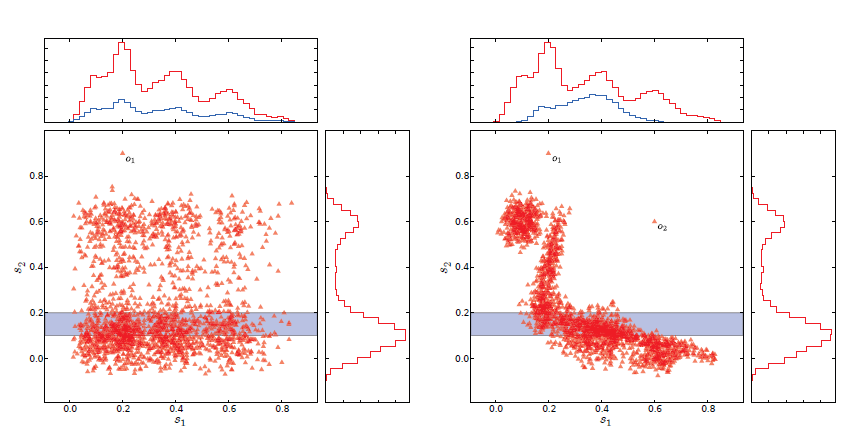
\includegraphics[scale=0.6]{imagenes/ejemplo_anomalia_probabilidad}
	\caption{Ejemplo de anomalía \cite{fabian_keller_hics:_2012}}
\end{figure}

Como se puede observar tenemos dos espacios: el izquierdo no presenta datos correlados y el derecho sí presenta correlación. Podemos ver que en ambos casos se comparte una anomalía etiquetada como $O_1$. Esta anomalía en el caso del espacio no correlado es perfectamente detectable de forma trivial observando las proyecciones de los datos en una dimensión. En cambio en el segundo caso ninguna de las dos anomalías etiquetadas $O_1 , O_2$ son detectables de esta forma trivial, pues si hacemos las proyecciones uno dimensionales ninguno de los dos datos es discordante en dichas proyecciones. Estas anomalías son las que decimos que son no triviales. En cambio si observamos los datos en una proyección de orden superior como la que estamos viendo de dimensión 2 podemos observar claramente que se salen de la correlación de datos que muestra el resto. Es aquí donde podemos ver que en el conjunto de la derecha ninguno de los puntos es una anomalía en las proyecciones de dimensión uno pero sí lo son en la proyección de dimensión 2.

Vamos por tanto a definir más formalmente este concepto especial de anomalía. Necesitamos introducir en primer lugar un poco de notación.

Partimos de un conjunto de datos $X = \{ x_1 , ... , x_n \}$ de $n$ objetos cada uno tomando $d$ valores, es decir, $x_i = (x_{s_1} , ... , x_{s_d}) \in \mathbb{R}^d$. Notamos un subespacio del conjunto de valores como:

$$S = \{ s_i | s_i \in \{ s_1 , ... , s_d \} \ con \ i\in \Delta \}$$

Dado un subespacio $S = \{ s_1 , ... , s_p \}$ notamos la proyección de los objetos del conjunto de datos como $X_{S} = \{ x_{s_1} , ... , x_{s_p} \}$.

Esta proyección está distribuida según una distribución conjunta desconocida de $S$:

$$p_{s_1 , ... , s_p} (x_{s_1} , ... , x_{s_p})$$

Notamos la distribución marginal asociada al atributo $s_i$ como:

$$p_{s_i}(x_{s_i})$$

\begin{definicion}
	Decimos que un subespacio $S$ es un espacio incorrelado si y sólo si:
	
	$$p_{s_1 , ... , s_p}(x_{s_1} , ... , x_{s_p}) = \prod_{i=1}^{p}p_{s_i}(x_{s_i})$$
\end{definicion}

Por tanto si estamos bajo la suposición de un espacio incorrelado podemos decir que la densidad esperada es:

$$p_{esp}(x_{s_1} , ... , x_{s_p}) \equiv \prod_{i=1}^{p}p_{s_i}(x_{s_i})$$

Recordemos que nuestras anomalías no triviales no están en este tipo de subespacios, si no en los correlados. Por tanto vamos a definirlo de la siguiente forma:

\begin{definicion}
	Decimos que un objeto $x_{S}$ es una anomalía no trivial respecto al subespacio $S$ si:
	
	$$p_{s_1 , ... , s_p}(x_{s_1} , ... , x_{s_p}) \ll p_{esp}(x_{s_1} , ... , x_{s_p})$$
	
	Es decir, si la probabilidad esperada es significativamente mayor que la probabilidad conjunta.
\end{definicion}

Por cómo hemos definido los espacios correlados e incorrelados es claro que no podemos tener anomalías en espacios no correlados como es evidente pues la densidad conjunta y esperada serían iguales.

Este concepto como podemos observar no comparte ninguna relación con nuestra definición de anomalías basadas en distancias por lo que es de esperar que si comparamos ambos tipos de anomalías en un conjunto de datos no obtengamos los mismos objetos.
%
\chapter{Modelos implementados}
\label{chapter:modelos}

En este capítulo vamos a repasar qué modelos he implementado y cómo funcionan cada uno de ellos. Primero se hará una revisión teórica de los modelos y posteriormente un análisis breve del código explicando las particularidades de las implementaciones.

\section{Algoritmos de ensamblaje}

Los algoritmos que he implementado pertenecen a una familia concreta de algoritmos de detección de anomalías denominados como algoritmos de ensamblaje o ``Ensemble Algorithms'' en inglés. Estos algoritmos son lo equivalente a los meta-algoritmos pero destinados a la detección de anomalías. Para dar una mejor definición de qué son los algoritmos de ensamblaje vamos a introducir una clasificación de los mismos para dar las categorías que entran dentro de esta definición.

\begin{itemize}
	\item Algoritmos de ensamblaje secuenciales: En este tipo de algoritmos tenemos un algoritmos base o un conjunto de algoritmos base que se aplican de forma secuencial, de forma que las primeras ejecuciones se ven usadas o modificadas por ejecuciones futuras de algoritmos. Finalmente el resultado puede ser una combinación ponderada de las valoraciones de los algoritmos o el resultado del último de ellos.
	
	
	\begin{algorithm}[H]{\textbf{Ensamblaje secuencial:}}
		\SetAlgoLined
		
		\textbf{Entrada: } Conjunto de datos $\mathcal{D}$, Algoritmos base $\mathcal{A}_1 , ... , \mathcal{A}_r$
		
		j=1
		
		\Repeat{fin}{
			Tomamos el algoritmo $\mathcal{A}_j$ según los resultados anteriores
			
			Tomamos el conjunto de datos modificado $f_j (\mathcal{D})$ de anteriores ejecuciones
			
			Ejecutamos el algoritmo $\mathcal{A}_j$ sobre $f_j (\mathcal{D})$
			
			j=j+1
			
		}
	
		\KwResult{Combinación de los resultados}
	\end{algorithm}
	\item Algoritmos de ensamblaje independientes: En este caso se emplean o bien diferentes instancias del mismo algoritmo o bien diferentes porciones de los datos que se emplearán de forma distinta. Se puede variar la instanciación por ejemplo dependiendo del subespacio sobre el que queramos ejecutarlo o dependiendo de las características de una porción concreta de los datos.
	
	\begin{algorithm}[H]{\textbf{Ensamblaje independiente:}}
		\SetAlgoLined
		
		\textbf{Entrada: } Conjunto de datos $\mathcal{D}$, Algoritmos base $\mathcal{A}_1 , ... , \mathcal{A}_r$
		
		j=1
		
		\Repeat{fin}{
			Tomamos el algoritmo $\mathcal{A}_j$
			
			Creamos el conjunto de datos modificado $f_j (\mathcal{D})$
			
			Ejecutamos el algoritmo $\mathcal{A}_j$ sobre $f_j (\mathcal{D})$
			
			j=j+1
			
		}
		
		\KwResult{Combinación de los resultados}
	\end{algorithm}
\end{itemize}

\section{Mahalanobis Kernel}

Este algoritmo está englobado dentro de la categoría de algoritmos basados en dependencia. Esta clase de algoritmos intenta estudiar las dependencias que existen entre atributos para así poder detectar las instancias u objetos que no tienen estas dependencias y marcarlos como anomalías.

Si intentamos visualizar esta dependencia entre atributos de forma gráfica lo que observaríamos es que los datos están alineados o posicionados en hiperplanos lineales o no lineales de la siguiente forma:

\begin{figure}[H]
	\centering
	\label{hiperplano}
	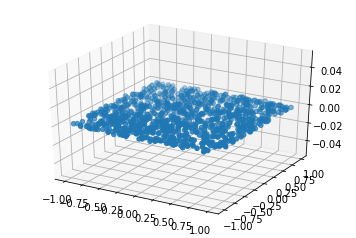
\includegraphics[scale=0.8]{imagenes/hiperplano}
	\caption{Hiperplano}
\end{figure}

Esta figura es un ejemplo clásico de estudio de algoritmos como por ejemplo PCA (algoritmo que quedaría dentro de esta categoría).

\begin{figure}[H]
	\centering
	\label{hiperboloide}
	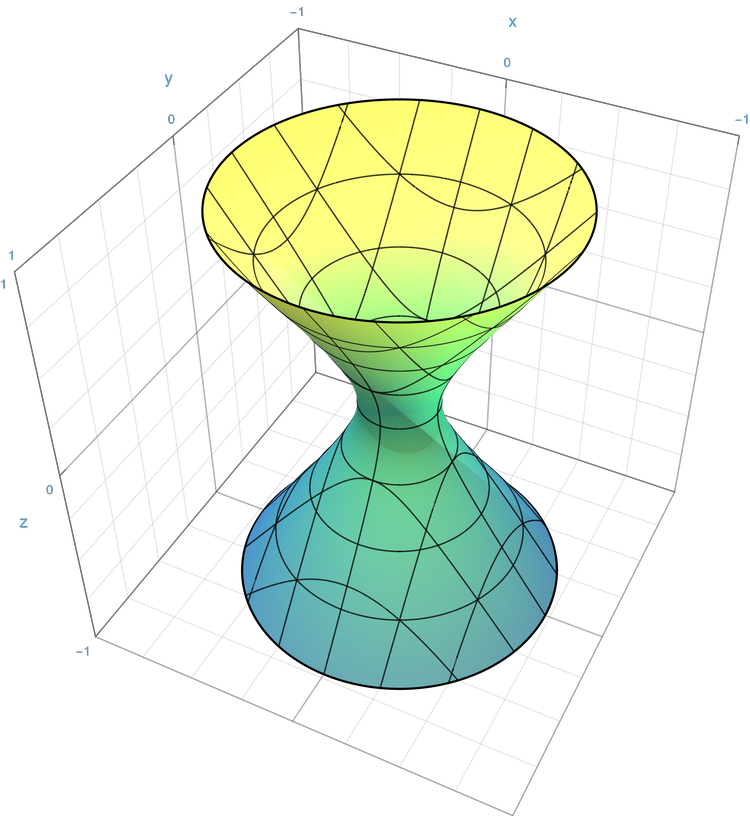
\includegraphics[scale=2.5]{imagenes/hiperboloide}
	\caption{Hiperboloide \href{https://commons.wikimedia.org/wiki/File:Circular_Hyperboloid_Of_One_Sheet_Quadric.png}{Wikimedia}}
\end{figure}

En este caso tenemos el ejemplo de un hiperboloide que no tiene una dependencia lineal, si no que presenta una dependencia de tipo cuadrático.

El método de Mahalanobis Kernel puede ser visto como una modificación de PCA. PCA básicamente dispone de dos pasos:

\begin{enumerate}
	\item Determinar un sistema ortogonal de direcciones principales y proyectar los datos sobre este sistema.
	\item Calcular la distancia entre el punto original y la proyección como su puntuación de anomalía.
\end{enumerate}

El método Mahalanobis Kernel intenta tener este mismo comportamiento en dos pasos y que ahora veremos. El algoritmo PCA es muy útil cuando los datos tienen atributos relacionados en un hiperplano, mientras que Mahalanobis Kernel funciona mejor cuando los datos están relacionados en formas más complejas como el hiperboloide que hemos enseñado. La elección de este algoritmo en vez de PCA recae en el hecho de que PCA es un algoritmo clásico y el escenario en el que mejor funciona (hiperplano) es más restrictivo que el que nos ofrece Mahalanobis Kernel con un abanico de figuras más amplio.

Vamos a describir el funcionamiento del algoritmo, pero primero vamos a introducir notación. Vamos a llamar $D$ a la matriz de datos que está centrada en la media y que tiene dimensiones $n\times d$, es decir, tenemos $n$ instancias u objetos de dimensionalidad $d$.

\begin{algorithm}[H]{\textbf{Mahalanobis Kernel}}
	\caption{Mahalanobis Kernel}
	\label{mahalanobis_kernel}
	\KwIn{$D$}
	
	$S = DD^T$.
	
	$S = Q\Delta^2 Q^T$.
	
	Almacenamos los vectores propios columna no negativos de $Q\Delta$ en una matriz $D'$
	
	Normalizamos $D'$ para que tenga media $0$ y varianza $1$.
	
	$vector\_media = media(D')$
	
	$puntuaciones = []$
	
	\ForEach{fila en D'}{
		$score = distancia(vector\_media , fila)$
		
		$puntuaciones = [puntuaciones, score]$
	}
	\KwOut{puntuaciones}
\end{algorithm}

El algoritmo comienza con la matriz de datos $D$. Se obtiene la matriz simétrica $S$ y se hace la descomposición en valores singulares. 

Con este modelo tenemos las dos fases que teníamos en PCA. Primero obtenemos una matriz $D'$ de los datos proyectados y transformados para posteriormente reportar la puntuación de anomalía como una distancia.

Veamos ahora la implementación en Python.

\begin{lstlisting}[language=Python]
def runMethod(self):
	'''
	@brief Function that executes the Kernel Mahalanobis method. The results are
	stored on the variable self.scores
	@param self
	'''
	''' Compute the S matrix of the algorithm'''
	S = np.dot(self.dataset, self.dataset.T)
	''' Now we diagonalize it'''
	Q,delta_sq,Qt = np.linalg.svd(S)
	del S
	del Qt
	''' Obtain delta as matrix'''
	delta = np.matrix(np.diag(np.sqrt(delta_sq)))
	del delta_sq
	Q = np.matrix(Q)
	''' Compute de D' matrix and normalize it'''
	Dprime = np.dot(Q,delta)
	del Q
	del delta
	Dp_std = scale(Dprime, axis=1)
	del Dprime
	''' We compute its mean on the rows to compute the deviation as the score'''
	mean = Dp_std.mean(axis=0)
	self.outlier_score=[]
	''' The score is the euclidean distance to the mean'''
	for i in range(len(Dp_std)):
		self.outlier_score.append(np.linalg.norm(mean-Dp_std[i])**2)
	self.outlier_score = np.array(self.outlier_score)
	self.calculations_done=True
\end{lstlisting}

La implementación del algoritmo se ha realizado en Python como el resto del proyecto y posteriormente se explicará en detalle cómo se ha organizado.

El algoritmo basa su implementación en la librería NumPy.

\section{TRINITY}

Este algoritmo es del segundo tipo que vimos al principio cuando hicimos una categorización de los algoritmos de ensamblaje, en concreto el algoritmo hace una combinación de tres componentes distintos. La intención de hacer esta composición de modelos es intentar obtener todos los tipos de anomalías que se puedan del conjunto y que reciban una puntuación acorde. La teoría nos dice que esta combinación de modelos nos va a proveer de un resultado más robusto que el uso de modelos aislados como discutiremos en la sección de resultados.

En concreto este algoritmo consta de tres componentes distintos:

\begin{itemize}
	\item Componente basado en distancias: este componente consta de un algoritmo que base su comportamiento en técnicas de agrupamiento o valoración por distancias como por ejemplo es el método clásico KNN. Este método lo que hace es tomar los k vecinos más cercanos y colocar como puntaje de anomalía para esa instancia como la suma de estas distancias. De esta forma los puntos que más alejados estén del resto sumarán una mayor distancia y por tanto serán más anómalos. En concreto este modelo se ha utilizado con el valor $k=5$ y con una técnica de subsampling. La técnica de subsampling consiste en no utilizar todo el conjunto de datos en el algoritmo, si no particionarlo y utilizar una pequeña muestra repitiendo este proceso y haciendo la media de las ejecuciones. De esta forma conseguimos una reducción de la varianza. Esto conlleva algunas ventajas como discutimos en la sección de sesgo y varianza anteriormente. En concreto la técnica toma 1000 particiones, ejecuta el algoritmo sobre ellas y hace la media.
	\item Componente basado en dependencia: este componente toma un algoritmo como el que hemos implementado (Mahalanobis Kernel). En este componente vamos a intentar detectar las anomalías que corresponden a datos que no siguen las relaciones entre atributos que sí tienen el resto de los objetos. Para ello he utilizado en este componente el algoritmo Mahalanobis Kernel que ya hemos explicado anteriormente incorporando la técnica de subsampling.
	\item Componente basado en densidad en subespacios: en este componente vamos a incorporar un modelo que intente buscar anomalías que lo sean en base a la densidad que tienen en alguno de los subespacios de los datos. Este hecho no nos debe ser ajeno pues es la segunda de las definiciones que hemos visto de anomalía y que hacía referencia a la función de densidad y los subespacios incorrelados y correlados. En concreto para este componente he utilizado el algoritmo IForest o Isolation Forest. Este algoritmo lo que hace es tomar de forma aleatoria un atributo y se van particionando los valores del mismo en una estructura de árbol, es decir, dividimos los datos en aquellos con un valor superior al marcado para el atributo y con un valor menor. De esta forma podemos medir cuántos pasos o lo que es lo mismo qué profundidad ha alcanzado nuestro árbol hasta llegar a dividir un objeto del resto de los datos. Este algoritmo también incorpora la técnica de subsampling.
\end{itemize}

Por último con esto hemos obtenido tres vectores o listas con la puntuación que cada componente nos ha arrojado para cada instancia. Para hacerlos comparables lo que debemos hacer es estandarizar los datos a media cero y varianza unitaria. Finalmente se realiza la media de los tres vectores de puntaje siendo esta la puntuación final devuelta por TRINITY.

Veamos la implementación de este algoritmo:

\begin{lstlisting}[language=Python]
def distanceBased(self):
	'''
	@brief Function that implements the distance based component
	@param self
	@return It returns the vector with the scores of the instances
	'''
	''' Initialize the scores'''
	scores = np.array([0]*len(self.dataset)).astype(float)
	for i in range(self.num_iter):
		knn = KNN(n_neighbors=5, contamination=self.contamination)
		''' Number in the interval [50, 1000]'''
		subsample_size = np.random.randint(50, 1001)
		sample = []
		if subsample_size>=len(self.dataset):
			sample = list(range(len(self.dataset)))
		else:
			''' Take the sample and train the model'''
			sample = np.random.choice(len(self.dataset), size=subsample_size, replace=False)
		knn.fit(self.dataset[sample])
		''' Update the score to compute the mean'''
		scores[sample]+=knn.decision_scores_
	''' Return the mean'''
	scores = scores/self.num_iter
	scores = scale(scores)
	return scores

def dependencyBased(self):
	'''
	@brief Function that implements the dependency based component
	@param self
	@return It returns the vector with the scores of the instances
	'''
	''' Initialize the scores'''
	scores = np.array([0]*len(self.dataset)).astype(float)
	for i in range(self.num_iter):
		kernel_mahalanobis = KernelMahalanobis(contamination=self.contamination)
		''' Number in the interval [50, 1000]'''
		subsample_size = np.random.randint(50, 1001)
		sample = []
		if subsample_size>=len(self.dataset):
			sample = list(range(len(self.dataset)))
		else:
			''' Take the sample and train the model'''
			sample = np.random.choice(len(self.dataset), size=subsample_size, replace=False)
		kernel_mahalanobis.fit(self.dataset[sample])
		''' Update the score to compute the mean'''
		scores[sample]+=kernel_mahalanobis.outlier_score
	''' Return the mean'''
	scores = scores/self.num_iter
	scores = scale(scores)
	return scores

def densityBased(self):
	'''
	@brief Function that implements the dependency based component
	@param self
	@return It returns the vector with the scores of the instances
	'''
	''' Initialize the scores'''
	scores = np.array([0]*len(self.dataset)).astype(float)
	for i in range(self.num_iter):
		iforest = IForest(contamination=self.contamination, behaviour="new")
		''' Number in the interval [50, 1000]'''
		subsample_size = np.random.randint(50, 1001)
		sample = []
		if subsample_size>=len(self.dataset):
			sample = list(range(len(self.dataset)))
		else:
			''' Take the sample and train the model'''
			sample = np.random.choice(len(self.dataset), size=subsample_size, replace=False)
		iforest.fit(self.dataset[sample])
		''' Update the score to compute the mean'''
		scores[sample]+=iforest.decision_scores_
	''' Return the mean'''
	scores = scores/self.num_iter
	scores = scale(scores)
	return scores

def runMethod(self):
	'''
	@brief This function is the actual implementation of TRINITY
	@param self
	'''
	''' Distance module'''
	if self.verbose:
		print("Obtaining scores with the distance module")
	distance_based = self.distanceBased()
	''' dependency module'''
	if self.verbose:
		print("Obtaining scores with the dependency module")
	dependency_based = self.dependencyBased()
	''' Density module'''
	if self.verbose:
		print("Obtaining scores with the density module")
	density_based = self.densityBased()
	
	''' Compute the mean of the three modules'''
	self.outlier_score=(distance_based + dependency_based + density_based)/3
	self.calculations_done=True
\end{lstlisting}

Todos los módulos tienen una función parecida. En primer lugar se inicializan las puntuaciones y se repite el mismo proceso de cálculo 100 veces. Se inicializa el modelo y se ajusta con una muestra de tamaño en el intervalo $[50,1000]$. Por último se hace la media de todos los cálculos y se estandarizan con la librería Sklearn.

En la función principal ``runMethod'' se ejecutan los tres módulos y se hace la media de las puntuaciones.

\section{OUTRES}

Este método entra dentro del segundo de los tipos que hemos visto en la clasificación inicial pues el objetivo es analizar los datos por subespacios. Una de las cosas que podremos ver al final cuando hagamos el estudio de los resultados es lo costoso de estos métodos, siendo este el primero que nos va a servir de ejemplo para visualizar este problema.

En primer lugar cabe decir que en el resto de algoritmos las puntuaciones reflejan el factor de anomalía en orden creciente, es decir, a mayor puntaje más anómalo es el dato y a menor puntaje menos anómalo se dice que es.

En este caso los puntajes van a estar en el intervalo $[0,1]$ siendo $0$ un puntaje para un dato lo más anómalo posible y $1$ un puntaje para un dato lo más normal posible. Daremos razones para que esto sea así cuando veamos el algoritmo.

\begin{algorithm}[H]{\textbf{OUTRES}}
	
	\KwIn{o: instancia, S: subespacio}
	
	\ForEach{$i\in (D \setminus S)$}{
	
		$S' = S\cup \{ i \}$
		
		\If{$S'$ es relevate}{
			
			$den(o, S') = \frac{1}{n} \sum_{p\in AN(o,S')} K_e (\frac{dist_{S'}(o,p)}{\epsilon (|S'|)})$
			
			$dev(o,S') = \frac{\mu - den(o,S')}{2\sigma}$
			
			\If{$dev(o,S')\geq 1$}{
				
				$r(o) = r(o) \cdot \frac{den(o,S')}{dev(o,S')}$
				
			}
		
			$OUTRES(o,S')$
			
		}
	
		\Else{
		
			Para recursividad
		
		}

	}
	
	\KwOut{r: puntajes}
	
	\caption{OUTRES}
	\label{outres}
\end{algorithm}

En primer lugar tenemos que definir qué son los espacios relevantes. Decimos que un subespacio $S$ es relevante si la proyección sobre ese subespacio no está distribuida de uniformemente. No podemos hacer un test de que toda la proyección esté distribuida uniformemente por lo que nos vamos a valer del siguiente teorema:

\begin{teorema}
	Sea $S$ un subespacio del conjunto de datos. Si $S$ está distribuido uniformemente entonces $\forall s_i \in S$ tenemos que la proyección uno-dimensional del conjunto de datos sobre $s_i$ está distribuida uniformemente.
\end{teorema}

Este teorema nos da la siguiente herramienta: si comprobamos que ninguna proyección uno-dimensional está distribuida uniformemente entonces podemos afirmar que $S$ está distribuido uniformemente. Para hacer estas comprobaciones uno-dimensionales lo hemos hecho mediante el test de Kolmogorov-Smirnov. 

Además el algoritmo incorpora un nuevo concepto. Los datos tienen mayor relevancia cuando los consideramos en subespacios y cuando los metemos dentro de lo que los autores llaman vecindarios adaptativos. La definición de un vecindario adaptativo es la siguiente:

\begin{definicion}
	Definimos para la instancia u objeto $o$ en el subespacio $S$ su vecindario adaptativo como:
	
	$$AN(o,S) = \{ p | dist_{S}(o,p)\leq \epsilon (|S|) \}$$
\end{definicion}

Donde $dist_{S}$ es la función distancia sobre los atributos $S$. Aquí tenemos una distancia máxima definida en función del cardinal del subespacio que viene dada de la siguiente forma:

$$\epsilon (|S|) = 0.5 \cdot \frac{h_{optimal}(|S|)}{h_{optimal}(2)}$$

Donde:

$$h_{optimal} (d) = (\frac{8\Gamma (\frac{d}{2} + 1)}{\pi^{\frac{d}{2}}}(d+4)(2\sqrt{\pi})^d) n^{\frac{-1}{d+4}}$$

Donde $\Gamma$ denota la función gamma y $n$ es el tamaño del conjunto de datos, es decir, el número de objetos o instancias.

Con esto ya tenemos la definición del vecindario adaptativo y el objeto de tenerlo es poder comprobar que el la instancia $o$ es relevante en el subespacio $S$ dentro de su vecindario adaptativo.

En cuanto a la definición de densidad tenemos la función $K_{\epsilon}$ que es el llamado Kernel de Epachenikov. Esta función está definida como:

$$K_{\epsilon}(x) = (1-x^2) \ \forall x<1$$

En cuanto al $\mu$ y $\sigma$ que aparecen en el cálculo de la desviación son la media y la desviación típica de las densidades en el vecindario adaptativo de $o$ en el subespacio $S$. Por tanto con la desviación estamos midiendo cómo de alejada está la instancia $o$ en densidad respecto del resto de las instancias de su vecindario adaptativo. Si esta densidad es mayor a dos desviaciones típicas entonces $dev(o,S')$ será mayor que $1$ y por tanto estaremos ante un dato anómalo.

Si este es el caso, al estar los puntajes de anomalías inicializados a 1 podemos actualizarlo multiplicando por un valor menor estricto que 1. En este caso este valor es $\frac{den(o,S')}{dev(o,S')}$. Como este valor es menor que 1 reducirá el puntaje y lo acercará más a una anomalía. De esta forma cuantas más veces se actualice su puntaje y cuanto menor puntaje obtenga con $\frac{den(o,S')}{dev(o,S')}$ más anómalo consideraremos el dato.

Finalmente si el subespacio era relevante significa que aún podemos aumentar más la dimensionalidad pues puede que nos queden subespacios de mayor orden que sigan sin estar distribuidos según una uniforme.

Como dato cabe decir que el algoritmo empieza en dimensión 2 y no en dimensión 1 pues en una única dimensión no tiene sentido estudiar la densidad ya que no vamos a sacar información de calidad.

Veamos la implementación

\begin{lstlisting}[language=Python]
def isRelevantSubspace(self, subspace, neighborhood):
	'''
	@brief Function that tells if a subspace is relevant, this is that the projection
	of the dataset over the subspace is not distributed uniformly in the neighborhood
	@param self
	@param subspace Subspace to check
	@param neighborhood neighborhood in which to check the projection
	@return It returns True if the subspace is relevant, False in other case.
	'''
	''' We check first if we have already considered this subspace. If so, it is not relevant anymore.'''
	for sub in self.checked_subspaces:
		if len(np.intersect1d(sub, subspace))==len(subspace):
			return False

	''' Make the projection'''
	projection = self.dataset[:,subspace][neighborhood]
	if len(projection)==0:
		return False
	''' We check for each subspace if the 1-dimensional data is uniformly distributed'''
	for i in range(len(subspace)):
		min = np.amin(projection[:,i].reshape(-1))
		max = np.amax(projection[:,i].reshape(-1))
		''' We do it using the Kolmogorov-Smirnov test'''
		d,p = kstest(projection[:,i], "uniform", args=(min, max-min))
		''' If the null hypothesis is not rejected, this means the data follow a uniform distribution'''
		if p<=self.alpha:
			return False
	return True

def computeHOptimal(self, d):
	'''
	@brief Function that calculates the Hoptimal
	@param self
	@param d Parameter, usually the dimensionality of the subspace
	@return It returns a numerical value.
	'''
	f1 = (8*gamma(d/2 + 1))/(np.power(np.pi, d/2))
	f2 = d+4
	f3 = np.power(2*np.sqrt(np.pi),d)
	n = len(self.dataset)
	f4 = np.power(n, -1/(d+4))
	return f1*f2*f3*f4

def computeEpsilon(self, subspace):
	'''
	@brief Function to compute the epsilon of the adapatative neighborhood
	@param self
	@params subspace Subspace considered to compute the epsilon
	@return It returns a numerical value
	'''
	return 0.5*(self.computeHOptimal(len(subspace))/self.computeHOptimal(2))

def computeNeighborhood(self, subspace, instance):
	'''
	@brief This function computes the adaptative neighborhood
	@param subspace Subspace in which to compute the neighborhood
	@param instance Instance considered as the centroid of the neighborhood (index of the element)
	@return It returns a numpy array containing the indexes of the neighborhood
	'''
	# First we compute the projection
	projection = self.dataset[:,subspace]
	# We compute a numpy array of the distances of all the elements to the instance
	tile = np.tile(projection[instance], len(self.dataset)).reshape((len(self.dataset),len(projection[instance])))
	distances = np.linalg.norm(projection-tile, axis=1)
	# We keep only the ones that are close enough (epsilon distance as max)
	neighborhood = np.where(distances<self.epsilons[len(subspace)])[0]
	# We exclude the instance itself
	return neighborhood[neighborhood!=instance]

def computeKernel(self, x):
	'''
	@brief Function that computes the Epanechnikov kernel with scalar factor 1
	@param self
	@param x Number between 0 and 1.
	@return It returns a numerical value
	'''
	return 1-np.power(x,2)

def computeDensity(self, subspace, neighborhood, instance):
	'''
	@brief This is the function that computes the density
	@param self
	@param subspace Subspace in which to compute the density
	@param neighborhood Adaptative neighborhood for the instance in the subspace
	@param instance Index of the instance considered at the moment
	@return It return a numerical value.
	'''
	# Compute the projection
	projection = self.dataset[:,subspace]
	# Compute the density
	tile = np.tile(projection[instance], len(self.dataset)).reshape((len(self.dataset),len(projection[instance])))
	return np.sum(self.computeKernel(np.linalg.norm(projection-tile, axis=1))/self.computeEpsilon(subspace))/len(self.dataset)

def computeDeviation(self, subspace, neighborhood, instance, density):
	'''
	@brief Function that computes the deviation
	@param self
	@param subspace Subspace considered to compute the deviation
	@param neighborhood Adaptative neighborhood for the instance in the subspace
	@param instance Instance to compute the deviation
	@param density Density value of the instance
	@return It returns a numerical value
	'''
	''' First we need to compute the density for all the neighbors'''
	densities = np.array([])
	for neig in neighborhood:
		local_neigborhood = self.computeNeighborhood(subspace, neig)
		densities = np.append(densities,self.computeDensity(subspace, local_neigborhood, neig))
	''' We compute the mean and the standard deviation'''
	mean = np.mean(densities)
	stdv = np.std(densities)
	''' Return the deviation'''
	return (mean-density)/(2*stdv)

def outres(self, instance, subspace):
	'''
	@brief Main loop of the outres algorithm
	@param self
	@param instance Instance to compute the outres score
	@param subspace Initial subspace of dimension 1
	'''
	''' First we compute the indexes of the features that are not used in the actual subspace'''
	available_indexes = list(set(list(range(len(self.dataset[0])))).difference(set(list(subspace))))
	''' For each available index we are going to check'''
	for index in available_indexes:
		''' We make the new subspace adding the index'''
		new_subspace = np.append(subspace, int(index)).astype(int)
		''' We compute the adaptative neighborhood'''
		neighborhood = self.computeNeighborhood(new_subspace, instance)
		''' If the subspace is relevant'''
		if self.isRelevantSubspace(new_subspace, neighborhood):
			''' Compute the density and deviation'''
			density = self.computeDensity(new_subspace, neighborhood, instance)
			deviation = self.computeDeviation(new_subspace, neighborhood, instance, density)
			''' If it is a high deviating instance in the subspace then we update the score'''
			if deviation>=1:
				if self.verbose:
					print("The instance " + str(instance+1) + " is outlying in the subspace " + str(new_subspace))
				''' The scores are equal to 1 at first and 1 means no outlierness and 0 means very outlying'''
				self.outlier_score[instance]*=density/deviation
			''' We keep the process if the subspace was relevant'''
			self.outres(instance, new_subspace)
		''' We add the subspace to the considered ones'''
		self.checked_subspaces.append(new_subspace)


def runMethod(self):
	'''
	@brief This function is the actual implementation of OUTRES
	'''
	''' First we compute all epsilons so we dont need to make this calculation more than once'''
	self.epsilons = [self.computeEpsilon(list(range(n))) for n in range(len(self.dataset[0])+1)]
	
	''' We initialize the scores to one'''
	self.outlier_score = np.ones(len(self.dataset))
	''' For each instance we run outres'''
	for i in range(len(self.dataset)):
		''' Erase checked_subspaces'''
		self.checked_subspaces = []
		if self.verbose and i%25==0:
			print("Computing the instance " + str(i+1) + "/" + str(len(self.dataset)))
		''' We run for each instance each index'''
		for j in range(len(self.dataset[0])):
			self.outres(i,np.array([j]))
	''' At the end, score 1 means no outlierness and 0 100% outlier. We make 1-score
	so we can keep the ascending order and now this will mean that 0 is no outlierness
	and 1 is very outlying.'''
	self.outlier_score = np.ones(len(self.dataset))-self.outlier_score
	self.calculations_done=True
\end{lstlisting}

\section{HICS}

HICS es otra aproximación distinta al estudio por subespacios como ha sido el algoritmo OUTRES. OUTRES intenta encontrar un subespacio interesante en el vecindario de una instancia, es decir, para cada instancia se busca el subespacio interesante para dicha instancia y no tiene por qué ser interesante para ninguna más. Esta aproximación es la opuesta pues la intención es buscar subespacios que sean interesantes en general y hacer una valoración de los datos sobre dichos subespacios.

Este algoritmo además pretende encontrar anomalías basándose en el concepto de densidad como introdujimos en la segunda definición de anomalía. Veamos primero el algoritmo en pseudocódigo para poder ir desgranándolo y explicarlo.

\begin{algorithm}[H]{\textbf{HICS}}
	
	\KwIn{D: dataset}
	
	$scores = [ \ ]$
	
	$sub = $ subespacios de alto contraste
	
	\ForEach{$S \in sub$}{
	
		Ajustamos un modelo con el algoritmo LOF con la proyección sobre $S$
		
		$scores = scores + puntaje \ LOF$
	
	}

	$scores = \frac{scores}{|sub|}$
	
	\KwOut{scores: puntajes}
	
	\caption{HICS}
	\label{hics}
\end{algorithm}

Como podemos ver el objetivo de HICS es en primer lugar obtener una serie de subespacios que sean relevantes y que hemos llamado subespacios de alto contraste. Para cada uno de estos subespacios vamos a estudiar la proyección de los datos sobre estos subespacios y vamos a obtener una puntuación de las instancias con el modelo LOF. Finalmente hacemos la media de todos estos puntajes para obtener la puntuación final. 

El modelo original está pensado para funcionar con LOF pero la teoría nos dice que podría funcionar con cualquier modelo basado en proximidad. Por tanto en la implementación desarrollada he incluido los modelos LOF, COF, CBLOF, LOCI, HBOS y SOD como alternativas entre las que elegir para la elección del modelo simple con el que obtener el puntaje.

Veamos ahora el pseudocódigo con el que obtenemos el contraste de un subespacio.

\begin{algorithm}[H]{\textbf{CalcularConstraste}}
	
	\KwIn{subespacio: subespacio, M: número de iteraciones del subsampling, $\alpha$: valor para obtener el tamaño de la muestra, $D$: conjunto de datos}
	
	$size = n \cdot \sqrt[|subespacio|]{\alpha}$
	
	$dev=0$
	
	\ForEach{$i\in [1,M]$}{
	
	$comp\_atr = aleatorio \ de \ subespacio$
	
	$sel\_obj = $ muestra aleatoria de $D$ de tamaño $size$
	
	$dev = dev + CalcularDev(comp\_atr, sel\_obj, subespacio, D)$
	
	}

	$dev = \frac{dev}{M}$
	
	\KwOut{$dev$: contraste}
	
	\caption{CalcularConstraste}
	\label{calcula_contraste}
\end{algorithm}

En resumen lo que vamos a ir haciendo es aplicar una técnica de subsampling en el algoritmo. Vamos a hacer $M$ ejecuciones para obtener el contraste tomando diferentes muestras de un tamaño fijado de antemano. Con estas muestras vamos a calcular la desviación del atributo de comparación $comp\_atr$ entre las instancias como vamos a ver ahora. Finalmente acumulamos toda esta desviación y obtenemos la media para ese subespacio. Con esto tenemos una medida de cuánto se desvían entre sí las instancias dentro de dicho subespacio.

\begin{algorithm}[H]{\textbf{CalcularDev}}
	
	\KwIn{$comp\_atr$: atributo con el que comparar, $sel\_obj$: muestra seleccionada aleatoriamente, $subespacio$: subespacio sobre el que calcular la desviación, $D$: conjunto de datos}
	
	$max = 0$
	
	\ForEach{$d\in D$}{
	
		$cum_1 = \sum_{o\in D} o[comp\_atr]$ si $o[comp\_atr]<d[comp\_atr]$
		
		$cum_2 = \sum_{o\in sel\_obj} o[comp\_atr]$ si $o[comp\_atr]<d[comp\_atr]$
		
		$f_a = \frac{cum_1}{|D|}$
		
		$f_b = \frac{cum_2}{|D|}$
		
		$subs = |f_a - f_b|$
		
		\If{$subs>max$}{
			
			$max = subs$
		
		}
	
	}
	
	\KwOut{max: máxima desviación}
	
	\caption{CalcularDev}
	\label{calcular_dev}
\end{algorithm}

Con este test lo que estamos haciendo es ver cómo se diferencia el atributo escogido para la comparación con cada instancia del resto del conjunto de datos. La idea es similar a la que expusimos cuando comentamos brevemente los Isolated Forests de ir dividiendo los datos con un valor de corte. 

Ahora ya tenemos las herramientas con las que podemos medir el contraste de un subespacio. Para ver cuáles son aquellos con mayor contraste los autores probaron dos formas quedándose finalmente con la que yo he añadido a la implementación. En primer lugar podemos pensar en algún tipo de cota que se vaya adaptando al número de subespacios o al contraste que estos vayan presentando. Esta idea finalmente fue descartada primero por no funcionar de forma satisfactoria y segundo por la dificultad de elección de la cota. La opción escogida finalmente es evaluar para cada dimensión todos los subespacios posibles, se obtiene el contraste de cada uno de ellos y se toma un número fijo de los primeros. De esta forma obtendremos por ejemplo en cada dimensión 500 candidatos. Una vez que hayamos evaluado todas las dimensiones volvemos a ordenar los subespacios por contraste (ya sin tener en cuenta la dimensionalidad) y nos quedamos con los 1000 primeros. Con esta metodología vamos a tener la certeza de que vamos a quedarnos con los 1000 subespacios con mayor contraste de entre todos los posibles. 

Veamos la implementación del algoritmo.

\begin{lstlisting}[language=Python]
def computeContrast(self, subspace):
	'''
	@brief Function that computes the contrast for a given subspace
	@param subspace Numpy array with the indexes of the features that define the subspace
	@return It returns a float representing the contrast of the subspace
	'''
	''' We set the adaptative size of the test'''
	size = int(len(self.dataset)*np.power(self.alpha, len(subspace)))
	''' Number of instances in the dataset'''
	N = len(self.dataset)
	deviation = 0
	''' We repeat the process M times'''
	for i in range(1,self.M+1):
		''' This is the comparison attribute for the test, so it will stay untouched'''
		comparison_attr=np.random.randint(low=0, high=len(subspace))
		''' List of booleans that masks the instances of the dataset selected'''
		selected_objects = np.array([True]*N)
		''' Select random indexes'''
		selected_objects[reduce(np.union1d,np.array([np.random.choice(N,size=size,replace=False) for _ in range(len(subspace)-1)]))]=False
		''' With the sample given by the mask selected_objects we compute the deviation'''
		deviation+=self.computeDeviation(subspace[comparison_attr], selected_objects, subspace)
	''' Finally the contrast is the average of all deviations'''
	return deviation/self.M

def computeDeviation(self, comparison_attr, selected_objects, subspace):
	'''
	@brief Function that computes the deviation of the marginal distribution
	given a fixed attribute, a sample and the condition given as a subspace
	@param comparison_attr This is the comparison attribute
	@param selected_objects Mask that sets a sample of the dataset
	@param subspace Subspace or condition to calculate the deviation
	@return It returns a float giving the deviation
	'''
	max = 0
	''' For each instance of the dataset'''
	for d in self.dataset:
		''' This is the cumulative value for all elements in the dataset'''
		cumul1 = np.sum(self.dataset[:,comparison_attr][self.dataset[:,comparison_attr]<d[comparison_attr]])
		''' This is the cumulative value for the selected_objects aka the sample'''
		sel = self.dataset[:,comparison_attr][selected_objects]
		cumul2 = np.sum(sel[sel<d[comparison_attr]])
		''' Finally we compute the average in both cases'''
		fa = cumul1/len(self.dataset)
		fb = cumul2/len(self.dataset)
		''' The difference in absolute value is the deviation'''
		subs = np.absolute(fa-fb)
		''' We return the biggest of the deviations obtained'''
		if subs>max:
			max = subs
	return max

def hicsFramework(self):
	'''
	@brief This function computes the high contrast subspaces on which to score the outlier
	@return It returns a numpy array containing the high contrast subspaces
	'''
	''' Ordered subspaces by dimension type: list of numpy arrays of numpy arrays
	 this means that in each positions there would be the subspaces of the corresponding
	 dimension in the form of a list of subspaces which are numpy arrays'''
	all_subspaces = []
	''' Record of the contrast for each subspace in each dimension, same shape as all_subspaces'''
	all_contrasts = []
	''' For all dimensions starting from dimension 2 (correlation has no sense on dimension 1)'''
	for dimension in range(2,len(self.dataset[0])):
		if self.verbose:
			print("Computing subspaces in dimension " + str(dimension) + "/" + str(len(self.dataset[0])))
		candidates = []
		contrasts = []
		''' This list will keep the indexes of the redundant subspaces, those are d-dimensional subspaces with d+1-dimensional
		 subspaces containing them with higher contrast'''
		redundant = []
		''' For dimension 2 we just obtain all possible indexes and make all combinations'''
		if dimension==2:
			''' Calculate the candidates as all possible combinations'''
			indexes = list(range(len(self.dataset[0])))
			candidates = np.array([np.array(list(comb)) for comb in list(combinations(indexes,dimension))])
			''' Compute the contrasts'''
			cont = 0
			p = Pool(self.numThreads)
			while cont+self.numThreads<len(candidates):
				contrasts = contrasts + p.map(self.computeContrast,candidates[cont:cont+self.numThreads])
				cont+=self.numThreads
				print("Computed " + str(cont) + "/" + str(len(candidates)))
			p = Pool(len(candidates)-cont)
			contrasts = contrasts + p.map(self.computeContrast,candidates[cont:])
			print("Computed " + str(len(candidates)) + "/" + str(len(candidates)))
		else:
			''' We need to calculate now the indexes starting from a previous subspace
			 We record the parent of each subspace to check for redundancy'''
			parents = []
			''' For all subspaces with one dimension less'''
			for i in range(len(all_subspaces[-1])):
				''' We only consider new indexes, those are the ones not uses in the father subspace'''
				indexes = list(set(list(range(len(self.dataset[0])))).difference(set(all_subspaces[-1][i])))
				''' For each new index'''
				for ind in indexes:
				''' We calculate the new candidate as the same subspace appending the index'''
				new_can = np.append(all_subspaces[-1][i],ind)
				''' Now we check that the candidate wasn't in the list before'''
				new = True
				for previous in candidates:
					if len(np.intersect1d(previous,new_can))==len(new_can):
						new = False
				if new:
					candidates.append(new_can)
					parents.append(i)
			''' Compute the contrasts'''
			cont = 0
			p = Pool(self.numThreads)
			while cont+self.numThreads<len(candidates):
				contrasts = contrasts + p.map(self.computeContrast,candidates[cont:cont+self.numThreads])
				cont+=self.numThreads
				print("Computed " + str(cont) + "/" + str(len(candidates)))
			p = Pool(len(candidates)-cont)
			contrasts = contrasts + p.map(self.computeContrast,candidates[cont:])
			print("Computed " + str(len(candidates)) + "/" + str(len(candidates)))
			
			''' Check for redundancy'''
			for i in range(len(parents)):
				if contrasts[i]>all_contrasts[-1][parents[i]]:
					redundant.append(parents[i])
		
		candidates = np.array(candidates)
		contrasts = np.array(contrasts)
		''' If there are redundant subspaces'''
		if redundant!=[]:
			if self.verbose:
				print("Now deleting redundant subspaces in dimension " + str(dimension) + ", " + str(len(redundant)) + " subspaces removed.")
		''' Delete those ones'''
		non_redundant_sub = np.delete(all_subspaces[-1], redundant)
		''' Update the subspaces'''
		all_subspaces[-1]=non_redundant_sub
		''' Sort from higher contrast to lower and only get numCandidates number of subspaces if available'''
		if len(candidates)>self.numCandidates:
			all_subspaces.append(candidates[contrasts.argsort()[-self.numCandidates:][::-1]])
			all_contrasts.append(contrasts[contrasts.argsort()[-self.numCandidates:][::-1]])
		else:
			all_subspaces.append(candidates)
			all_contrasts.append(contrasts)
	''' We flatten the numpy array to obtain only a list of subspaces and contrasts'''
	subspaces = np.array(all_subspaces).flatten()
	contrasts = np.array(all_contrasts).flatten()
	''' We only give the maxOutputSpaces with higher contrast if available'''
	if len(subspaces)>self.maxOutputSpaces:
		return subspaces[contrasts.argsort()[-self.maxOutputSpaces:][::-1]]
	return subspaces

def runMethod(self):
	'''
	@brief This function is the actual implementation of HICS
	'''
	if self.verbose:
		print("Calculating the subspaces\n")
	''' First we obtain the high contrast subspaces'''
	subspaces = self.hicsFramework()
	
	if self.verbose:
		print("Now calculating the scoring\n")
	''' We initialize the scores for each instance as 0'''
	scores = np.zeros(len(self.dataset))
	''' For each subspace'''
	for sub in subspaces:
		''' We place the corresponding scorer according to parameter'''
		scorer = None
		if self.outlier_rank=="lof":
			scorer = LOF()
		elif self.outlier_rank=="cof":
			scorer = COF()
		elif self.outlier_rank=="cblof":
			scorer = CBLOF()
		elif self.outlier_rank=="loci":
			scorer = LOCI()
		elif self.outlier_rank=="hbos":
			scorer = HBOS()
		elif self.outlier_rank=="sod":
			scorer = SOD()
		''' Fits the scorer with the dataset'''
		scorer.fit(self.dataset[:,sub])
		''' Adds the scores obtained to the global ones'''
		scores = scores+scorer.decision_scores_
	''' Compute the average'''
	self.outlier_score = scores/len(subspaces)
	''' Marks the calculations as done'''
	self.calculations_done=True
\end{lstlisting}

\section{LODA}

LODA es un algoritmo que entra en la categoría de los algoritmos que involucran histogramas. Aún no hemos visto ningún algoritmo de este tipo, por lo que no hemos discutido el funcionamiento de estos algoritmos. Cuando hacemos un histograma de los datos estudiamos la distribución de probabilidad de los datos y por tanto podemos ver si éstos están en las colas en algún atributo o proyección o si están en el centro de la distribución. Con esto podemos saber si el dato es o no anómalo. En concreto LODA emplea una serie de proyecciones uno-dimensionales sobre las que se estudia la distribución. 

En primer lugar vamos a ver cómo se obtienen los vectores que nos dan las proyecciones uno-dimensionales.

\begin{algorithm}[H]{\textbf{ProyeccionesAleatorias}}
	
	\KwIn{$d$: dimension, $D$: dataset, $k$: número de histogramas y proyecciones}
	
	$no\_neg = [\sqrt{d}]$
	
	$proyecciones = [ \ ]$
	
	\ForEach{$i\in [1,k]$}{
	
		$ind = $ $no\_neg$ indices aleatorios en $[0,d]$
		
		$proy = $ vector con ceros en todas las posiciones menos en ind, donde hay valores sacados de una normal $\mathcal{N}(0,1)$
		
		$proyecciones = [proecciones, proy]$

	}
	
	\KwOut{$proyecciones$: proyecciones}
	
	\caption{ProyeccionesAleatorias}
	\label{proyecciones_aleatorias}
\end{algorithm}

En LODA tenemos un parámetro $k$ que nos indica el número de proyecciones e histogramas que vamos a desarrollar. Esto nos va a dar más o menos muestras como haríamos con una técnica de subsampling tradicional. 

Una vez que tenemos estos vectores de proyección vamos a ver cómo generamos los histogramas a partir de ellos.

\begin{algorithm}[H]{\textbf{ObtenerHistogramas}}
	
	\KwIn{$D$: dataset, $\{w_i\}_{i=1}^{k}$: vectores de proyecciones, $k$: numero de histogramas y vectores de proyección}
	
	Inicializamos los histogramas $\{h_i\}_{i=1}^{k}$
	
	\For{$j=1 \rightarrow |D|$}{
	
		\For{$i=1\rightarrow k$}{
		
			$z_i = x_j^T w_i$	
			
			Actualiza el histograma $h_i$ con $z_i$

		}

	}
	
	\KwOut{$\{h_i\}_{i=1}^{k}$: histogramas}
	
	\caption{ObtenerHistogramas}
	\label{obtener_histogramas}
\end{algorithm}

Con esto ya tenemos tanto las proyecciones como los histogramas, por lo que sólo queda ver cómo obtenemos las puntuaciones de anomalías de los datos.

\begin{algorithm}[H]{\textbf{LODA}}
	
	\KwIn{$x$: instancia, $\{h_i\}_{i=1}^{k}$: histogramas, $\{w_i\}_{i=1}^{k}$: vectores de proyección}
	
	\For{$i=1\rightarrow k$}{
	
		$z_i = x^T w_i$
		
		Obtenemos $p_i = p_i (z_i)$ del histograma $h_i$

	}

	$f = \frac{-1}{k} \sum_{i=1}^{k}\log (p_i (z_i))$
	
	\KwOut{$f$: puntaje de anomalía de $x$}
	
	\caption{LODA}
	\label{loda}
\end{algorithm}

Finalmente ya tenemos el algoritmo LODA completo. Cuando estamos evaluando una instancia obtenemos la probabilidad de que su proyección uno-dimensional ocurra. Con esta probabilidad si hacemos el logaritmo cuanto más cerca esté de $0$ más cerca estará el valor de $-\infty$ y por tanto mayor va a ser nuestro puntaje anómalo de dicha instancia.

Ahora que ya tenemos el algoritmo completo vamos a ver la implementación:

\begin{lstlisting}[language=Python]
def getRandomProjections(self, dimension):
	'''
	@brief Function that computes and returns the random projections
	@param self
	@param dimension Dimensionality of the dataset (int)
	@return It returns a list with numpy arrays as projections
	'''
	''' Number of non-negative elements in the projection'''
	non_neg = int(np.ceil(np.sqrt(dimension)))
	projections = []
	''' We are going to compute k projections'''
	for i in range(self.k):
		''' Select non_neg random indexes to make the projection'''
		ind = np.random.choice(dimension, replace=False, size=non_neg)
		''' Initialize it to zeroes'''
		proj = np.zeros(dimension)
		''' The non-negative elements are drawn from a normal distribution'''
		proj[ind]=np.random.normal(size=non_neg)
		projections.append(proj)
	return projections

def getBin(self, hist_limits, value):
	'''
	@brief Function that given a value, it returns the bin it belongs to for the histogram
	@param self
	@param hist_limits Limits for each bin of the histogram
	@param value Value to check for the bin
	@return It returns the index corresponding to the bin
	'''
	bin=-1
	for i in range(len(hist_limits)):
		if value<hist_limits[i]:
			bin=i
			break
	return bin-1

def runMethod(self):
	'''
	@brief This is the implementation of the LODA algorithm
	'''
	''' We compute first all projections'''
	random_projections = self.getRandomProjections(len(self.dataset[0]))
	''' Initialize the histograms and the projected data'''
	histograms = [[]]*self.k
	Z = [[]]*self.k
	''' For each instance of the dataset'''
	for j in range(len(self.dataset)):
		''' For each projection'''
		for i in range(self.k):
			''' Compute the 1D projection'''
			Z[i].append(np.dot(self.dataset[j].T, random_projections[i]))
	''' Compute the k histograms with the data'''
	for i in range(self.k):
		histograms[i]=np.histogram(Z[i], bins = self.n_bins)
	
	''' Initialize the scores to zero'''
	self.outlier_score = np.array([0]*len(self.dataset)).astype(float)
	''' For each instance'''
	for i in range(len(self.dataset)):
		prob = []
		''' For each histogram'''
		for j in range(self.k):
			''' Compute the projection'''
			z = np.dot(self.dataset[i].T, random_projections[j])
			''' Check the bin for the projection'''
			bin = self.getBin(histograms[j][1], z)
			''' Obtain the probability linked to z in the histogram'''
			prob.append(histograms[j][0][bin]/np.sum(histograms[j][0]))
		prob = np.array(prob)
		''' Compute the score with the probabilities'''
		if 0. in prob:
			self.outlier_score[i] = float("inf")
		else:
			self.outlier_score[i] = -np.sum(np.log(prob))/self.k
	self.calculations_done=True
\end{lstlisting}

\section{Implementación}

Todos los algoritmos están implementados utilizando una clase base llamada EnsembleTemplate:

\begin{lstlisting}[language=Python]
class EnsembleTemplate:
'''
Template class for the ensemble anomaly detectors.
'''

def __init__(self, contamination=0.1):
	'''
	Init template
	'''
	pass

def fit(self, dataset):
	'''
	Function to set the dataset and execute the algorithm
	'''
	self.dataset = dataset
	self.outlier_score = [0]*len(self.dataset)
	self.outliers = []
	self.runMethod()
	return self

def runMethod(self):
	'''
	Function to run the method implemented
	'''
	pass

def getRawScores(self):
	'''
	Function that gets the raw scores
	'''
	return self.outlier_score

def getOutliersBN(self, noutliers):
	'''
	Function that gets the noutliers instances of the most outlying data
	'''
	return self.outliers

def getOutliers(self):
	pass
\end{lstlisting}

El esqueleto de todas las clases que implementan los algoritmos de los que hemos hablado es este. En primer lugar todas las clases tienen un constructor en el que se pasan los parámetros de los modelos en caso de haberlos. En segundo lugar tenemos una función fit. El cometido de esta función es inicializar los puntajes, pasar el dataset al objeto de la clase para que se guarde y por último ejecutar el método que implementa.

La función principal es la función runMethod que es la que implementa la ejecución del algoritmo en sí. Esta función no está pensada para ser llamada externamente si no desde fit. 

Por último tenemos tres funciones más. La primera de ellas nos da el vector que contiene los puntajes de las anomalías. La segunda función nos da los ``noutliers'' elementos con mayor puntaje y la tercera nos devuelve las instancias anómalas basándose en un parámetro que llamamos contaminación. 

El parámetro de contaminación no es más que una estimación del porcentaje de anomalías que pensamos que va a tener el conjunto de datos. Por tanto si el parámetro de contaminación fuera por ejemplo $0.1$ entonces esta función devolvería el primer $10\%$ con mayor valor de puntaje de anomalía.

Toda la implementación del trabajo se encuentra alojada en GitHub en \href{https://github.com/nacheteam/Ensemble-Outlier-Analysis}{\textbf{\underline{este repositorio}}}.
%
\chapter{Experimentación y Resultados}
\label{chapter:experimentacion_resultados}

\section{Conjuntos de datos}

Para comenzar la experimentación vamos a hacer un repaso de los conjuntos de datos y la técnica seguida para realizar la misma. En primer lugar cabe decir que al ser un problema no supervisado en origen no tendríamos forma de saber nuestro acierto en el problema. En este tipo de casos hay dos aproximaciones: estimar el acierto o utilizar conjuntos que sí están clasificados y obtener de esta forma el acierto. La segunda de las alternativas es la que vamos a seguir en este estudio y es la que se suele denominar como problema semi-supervisado. 

Para tomar este camino necesitamos conjuntos en los que tengamos disponible la clasificación de datos anómalos y no anómalos. Estos conjuntos de datos han sido tomados de la web Outlier Detection Datasets \cite{shebuti_ryana_odds_2016}, librería mantenida por la universidad Stony Brooks.

Estos conjuntos de datos están en formato Matlab, formato que puede ser fácilmente leído por la librería SciPy. Estos conjuntos de datos vienen con información de cabecera, versión e incluso algunos con una breve descripción o resumen si dispusieran de ella. Lo importante es que los datos vienen divididos en dos, primero un vector que contiene una lista con los vectores que componen los datos y en segundo lugar un vector con las etiquetas donde $0$ significa que el dato no es anómalo y $1$ que sí lo es.

\begin{figure}[H]
	\centering
	\label{dataset_matlab}
	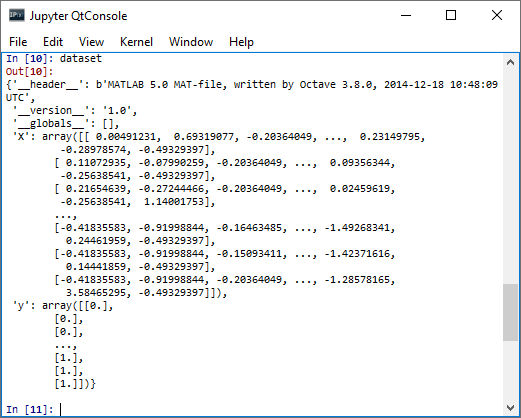
\includegraphics[scale=0.8]{imagenes/datasets_matlab}
	\caption{Contenido de los conjuntos de datos}
\end{figure}

Como podemos ver ``X'' contiene el conjunto de datos y el campo ``y'' contiene las etiquetas para los mismos.

En algunos de estos conjuntos de datos podemos encontrar lo que conocemos como valores perdidos o en inglés ``missing values''. Estos valores vienen reflejados con ``NAN'' en los conjuntos. Estos valores no sólo no nos son de interés si no que además nuestros modelos no están preparados para poder trabajar con ellos por lo que tenemos que decidir que transformación aplicamos para poder emplear los conjuntos de datos. La decisión tomada para estos valores ha sido la de eliminar las instancias que presenten valores perdidos. Esta decisión se basa en que, si estas instancias son anómalas no tenemos forma alguna de tratar con ellas porque no disponen de valores numéricos en sus campos y por tanto nuestros modelos no son aptos para resolver el conflicto. Esto no excluye el hecho de que estas instancias puedan ser anomalías reales. Por ejemplo pensemos en un sistema de frenos que sufre una rotura de alguno de sus sistemas. Si estos sistemas poseen sensores que recopilan datos es muy probable que estos sensores no tomen valores y por tanto dispongamos de valores perdidos precisamente porque la instancia es anómala. Esto se discutirá un poco más en profundidad cuando hablemos del trabajo futuro, de momento la decisión ha sido suprimir estas instancias.

Dentro de todos los conjuntos de datos que contiene la librería nosotros vamos a utilizar los siguientes:

\begin{table}[H]
	\begin{tabular}{|l|l|l|}
		\hline
		\multicolumn{1}{|c|}{{\ul \textbf{Nombre}}} & \multicolumn{1}{c|}{{\ul \textbf{Dimensionalidad}}} & \multicolumn{1}{c|}{{\ul \textbf{Número de instancias}}} \\ \hline
		annthyroid                                  & 6                                                   & 7200                                                     \\ \hline
		arrhythmia                                  & 274                                                 & 452                                                      \\ \hline
		breastw                                     & 9                                                   & 683                                                      \\ \hline
		cardio                                      & 21                                                  & 1831                                                     \\ \hline
		glass                                       & 9                                                   & 214                                                      \\ \hline
		ionosphere                                  & 33                                                  & 351                                                      \\ \hline
		letter                                      & 32                                                  & 1600                                                     \\ \hline
		lympho                                      & 18                                                  & 148                                                      \\ \hline
		mammography                                 & 6                                                   & 11183                                                    \\ \hline
		mnist                                       & 100                                                 & 7603                                                     \\ \hline
		musk                                        & 166                                                 & 3062                                                     \\ \hline
		optdigits                                   & 64                                                  & 5216                                                     \\ \hline
		pendigits                                   & 16                                                  & 6870                                                     \\ \hline
		pima                                        & 8                                                   & 768                                                      \\ \hline
		satellite                                   & 36                                                  & 6435                                                     \\ \hline
		satimage-2                                  & 36                                                  & 5803                                                     \\ \hline
		speech                                      & 400                                                 & 3686                                                     \\ \hline
		thyroid                                     & 6                                                   & 3772                                                     \\ \hline
		vertebral                                   & 6                                                   & 240                                                      \\ \hline
		vowels                                      & 12                                                  & 1456                                                     \\ \hline
		wbc                                         & 30                                                  & 378                                                      \\ \hline
		wine                                        & 13                                                  & 129                                                      \\ \hline
	\end{tabular}
\end{table}

Como podemos ver hay algunos conjuntos con un tamaño razonablemente grande tanto en dimensionalidad como en número de instancias. Esto será discutido modelo por modelo pues los algoritmos basados en subespacios tienen una complejidad dependiente del factorial de la dimensionalidad, es decir, a partir de una cierta dimensionalidad el tiempo que consumen estos algoritmos es demasiado alto.

\section{Experimentación}

Sobre estos conjuntos de datos hemos ejecutado nuestros cinco modelos implementados: HICS, OUTRES, Mahalanobis Kernel, Trinity y LODA. Sobre estas ejecuciones se ha recopilado el porcentaje de acierto sobre ellos, el tiempo consumido en la ejecución y las propias puntuaciones dadas sobre estos conjuntos de datos por los modelos.

Para poder hacer la comparativa con los datos de nuestros modelos he tomado modelos clásicos. Estos modelos se han cogido de la librería PyOD \cite{zhao_pyod:_2019}. De esta librería se han tomado 10 modelos: Angle-Based Outlier Detection (ABOD), Connectivity-Based Outlier Factor (COF), Histogram-Based Outlier Score (HBOS), K Nearest Neighbors (KNN), Local Outlier Factor (LOF), Minimum Covariance Determinant (MCD), One-Class Support Vector Machines (OCSVM), Principal Component Analysis (PCA), Subspace Outlier Detection (SOD) y Stochastic Outlier Selection (SOS). Sobre estos modelos se ha recopilado exactamente la misma información que sobre los nuestros, es decir, el acierto, el tiempo consumido y las puntuaciones de las instancias.

En cuanto a OUTRES podemos estudiar cuándo un subespacio es importante para una instancia completa. Por tanto hemos lanzado otro experimento para intentar analizar los subespacios que son más relevantes para una determinada instancia.

\section{Resultados}

En primer lugar vamos a ver los resultados que obtenemos de todos los modelos sobre todos los conjuntos de datos. Se muestra un gráfico de barras por cada conjunto de datos con el desempeño de cada modelo. Cabe decir que tanto OUTRES como HICS son algoritmos como hemos comentado con una eficiencia muy mala en tiempo. Al ser su complejidad en tiempo dependiente del factorial de la dimensionalidad sólo hemos ejecutado el algoritmo en conjuntos de datos de baja dimensionalidad para poder completar dicha ejecución en un tiempo razonable, aunque como veremos hay algunos conjuntos de datos cuya ejecución ha llevado varias horas.

Veamos primero todos los gráficos con los resultados para poder analizarlos y particularizar posteriormente.

\begin{figure}[H]
	\centering
	\label{annthyroid_accuracy}
	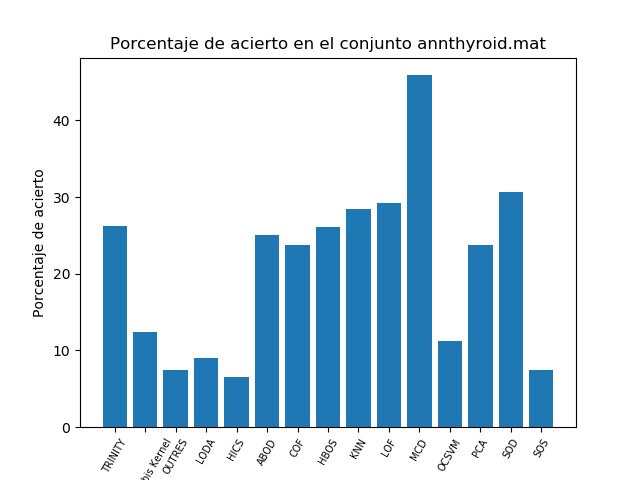
\includegraphics[scale=0.7]{imagenes/imgs-exp1/accuracy/annthyroid}
	\caption{Porcentaje de acierto sobre el conjunto de datos annthyroid}
\end{figure}

\begin{figure}[H]
	\centering
	\label{arrhythmia_accuracy}
	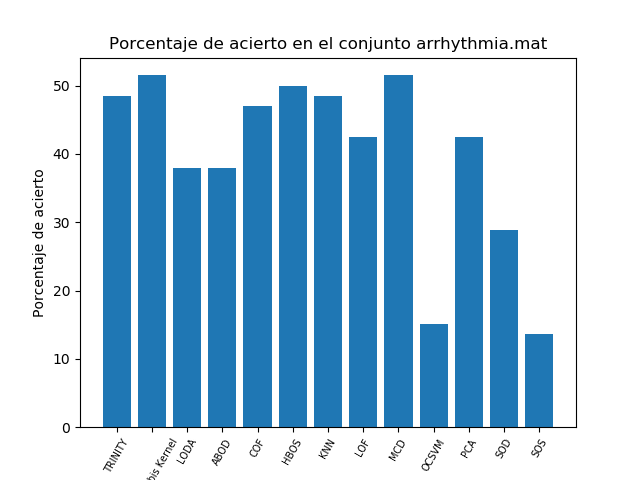
\includegraphics[scale=0.7]{imagenes/imgs-exp1/accuracy/arrhythmia}
	\caption{Porcentaje de acierto sobre el conjunto de datos arrhythmia}
\end{figure}

\begin{figure}[H]
	\centering
	\label{breastw_accuracy}
	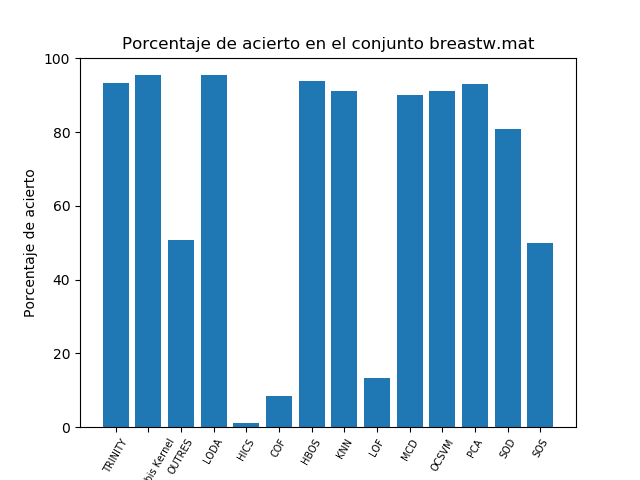
\includegraphics[scale=0.7]{imagenes/imgs-exp1/accuracy/breastw}
	\caption{Porcentaje de acierto sobre el conjunto de datos breastw}
\end{figure}

\begin{figure}[H]
	\centering
	\label{cardio_accuracy}
	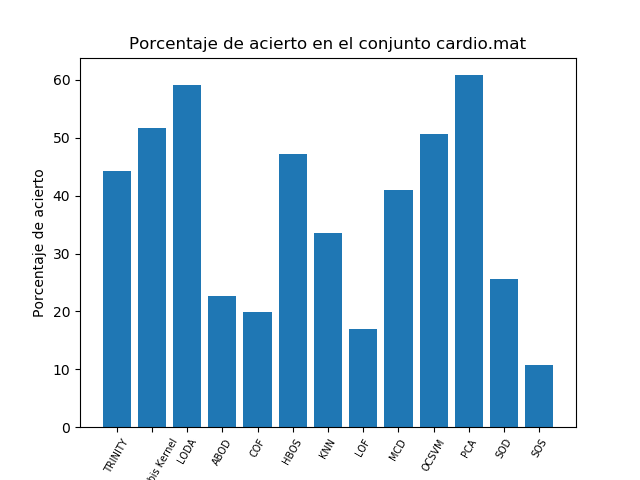
\includegraphics[scale=0.7]{imagenes/imgs-exp1/accuracy/cardio}
	\caption{Porcentaje de acierto sobre el conjunto de datos cardio}
\end{figure}

\begin{figure}[H]
	\centering
	\label{glass_accuracy}
	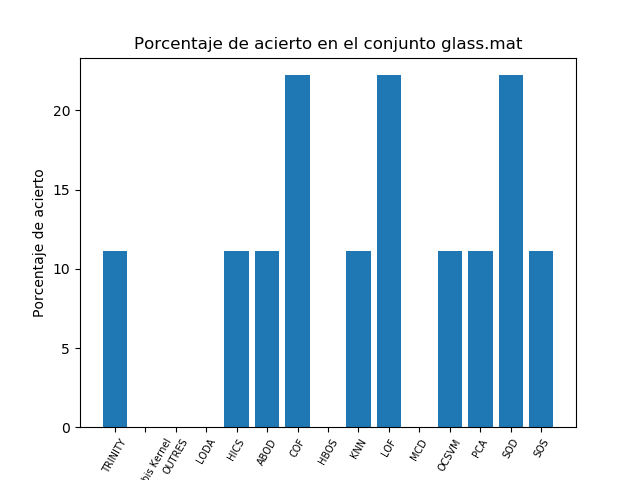
\includegraphics[scale=0.7]{imagenes/imgs-exp1/accuracy/glass}
	\caption{Porcentaje de acierto sobre el conjunto de datos glass}
\end{figure}

\begin{figure}[H]
	\centering
	\label{ionosphere_accuracy}
	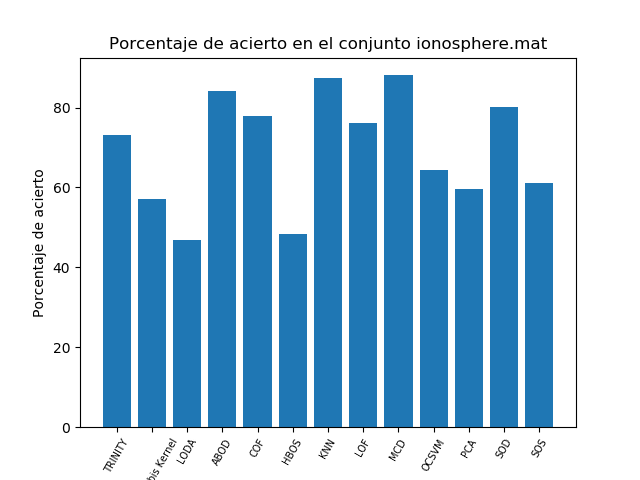
\includegraphics[scale=0.7]{imagenes/imgs-exp1/accuracy/ionosphere}
	\caption{Porcentaje de acierto sobre el conjunto de datos ionosphere}
\end{figure}

\begin{figure}[H]
	\centering
	\label{letter_accuracy}
	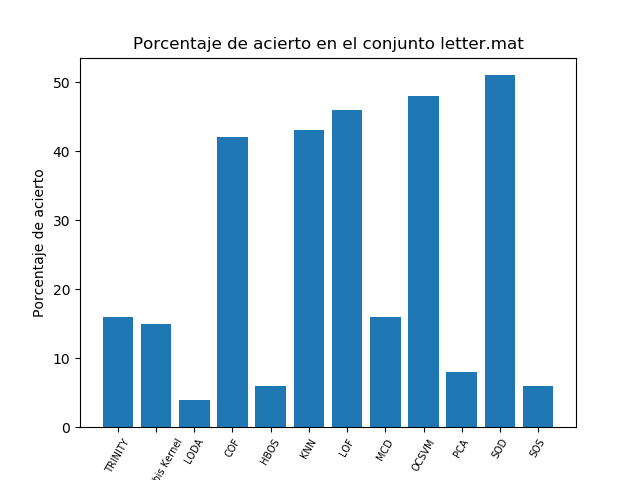
\includegraphics[scale=0.7]{imagenes/imgs-exp1/accuracy/letter}
	\caption{Porcentaje de acierto sobre el conjunto de datos letter}
\end{figure}

\begin{figure}[H]
	\centering
	\label{lympho_accuracy}
	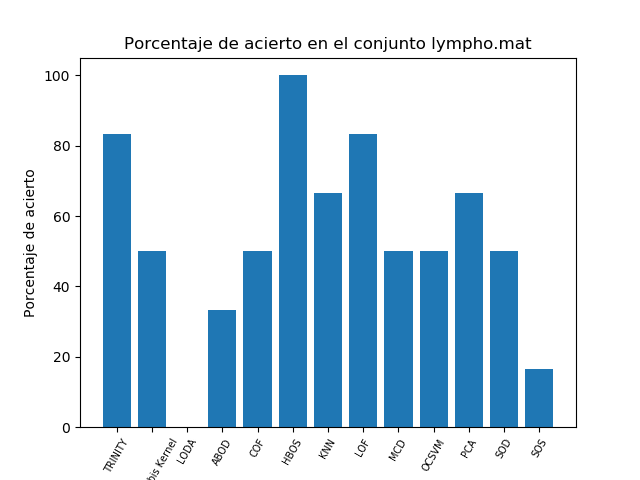
\includegraphics[scale=0.7]{imagenes/imgs-exp1/accuracy/lympho}
	\caption{Porcentaje de acierto sobre el conjunto de datos lympho}
\end{figure}

\begin{figure}[H]
	\centering
	\label{mammography_accuracy}
	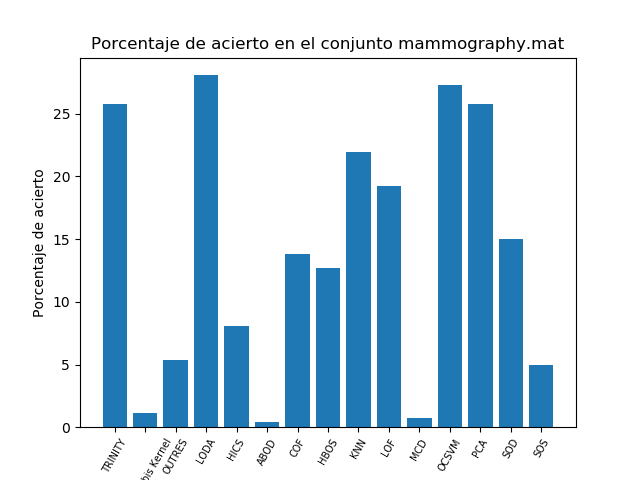
\includegraphics[scale=0.7]{imagenes/imgs-exp1/accuracy/mammography}
	\caption{Porcentaje de acierto sobre el conjunto de datos mammography}
\end{figure}

\begin{figure}[H]
	\centering
	\label{mnist_accuracy}
	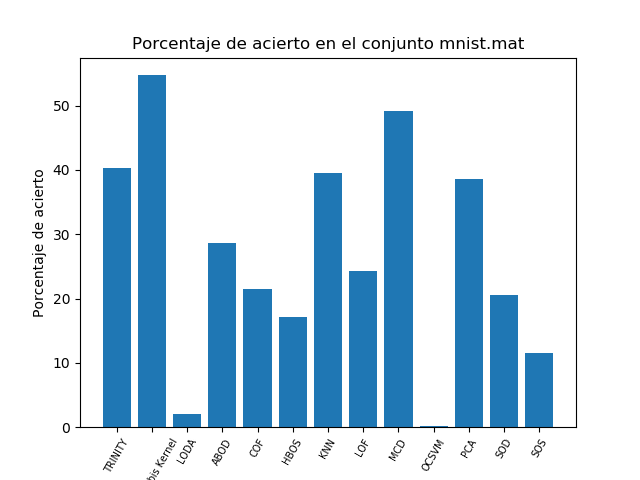
\includegraphics[scale=0.7]{imagenes/imgs-exp1/accuracy/mnist}
	\caption{Porcentaje de acierto sobre el conjunto de datos mnist}
\end{figure}

\begin{figure}[H]
	\centering
	\label{musk_accuracy}
	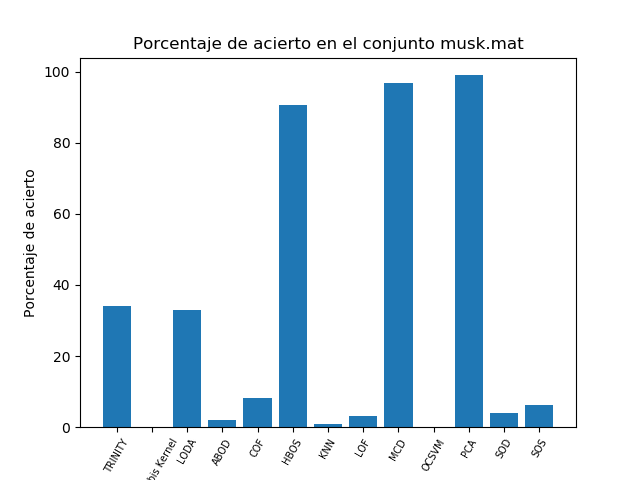
\includegraphics[scale=0.7]{imagenes/imgs-exp1/accuracy/musk}
	\caption{Porcentaje de acierto sobre el conjunto de datos musk}
\end{figure}

\begin{figure}[H]
	\centering
	\label{optdigits_accuracy}
	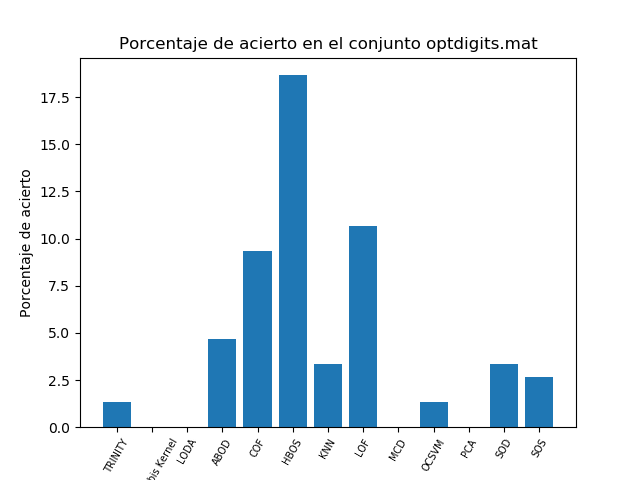
\includegraphics[scale=0.7]{imagenes/imgs-exp1/accuracy/optdigits}
	\caption{Porcentaje de acierto sobre el conjunto de datos optdigits}
\end{figure}

\begin{figure}[H]
	\centering
	\label{pendigits_accuracy}
	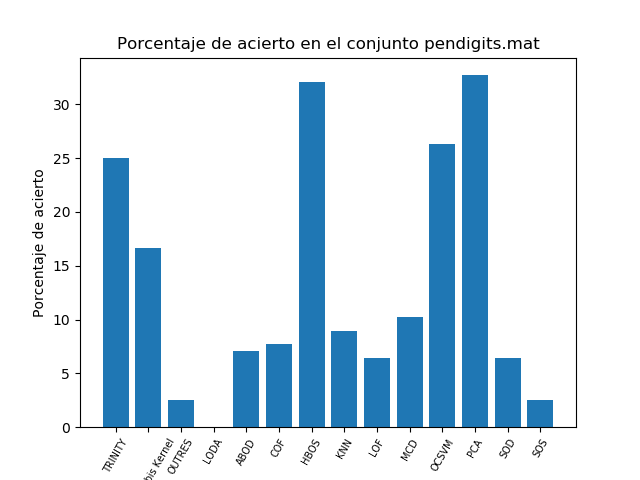
\includegraphics[scale=0.7]{imagenes/imgs-exp1/accuracy/pendigits}
	\caption{Porcentaje de acierto sobre el conjunto de datos pendigits}
\end{figure}

\begin{figure}[H]
	\centering
	\label{pima_accuracy}
	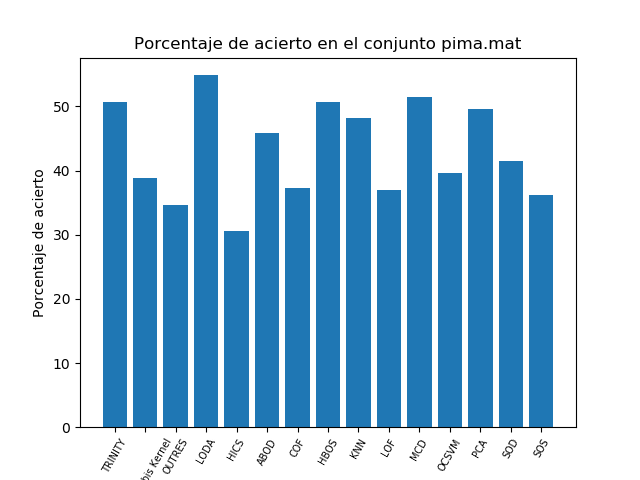
\includegraphics[scale=0.7]{imagenes/imgs-exp1/accuracy/pima}
	\caption{Porcentaje de acierto sobre el conjunto de datos pima}
\end{figure}

\begin{figure}[H]
	\centering
	\label{satellite_accuracy}
	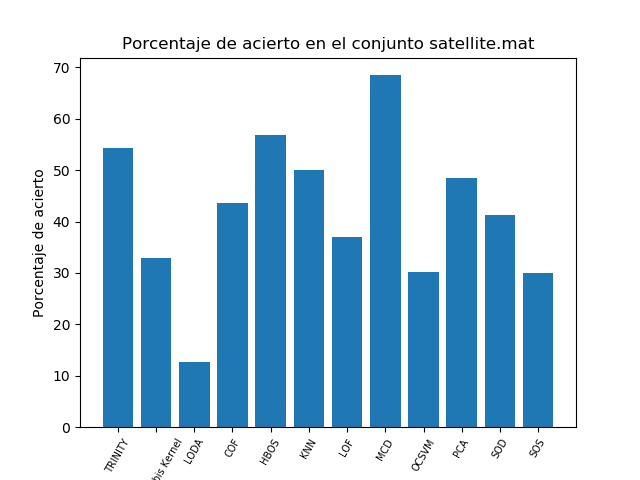
\includegraphics[scale=0.7]{imagenes/imgs-exp1/accuracy/satellite}
	\caption{Porcentaje de acierto sobre el conjunto de datos satellite}
\end{figure}

\begin{figure}[H]
	\centering
	\label{satimage-2_accuracy}
	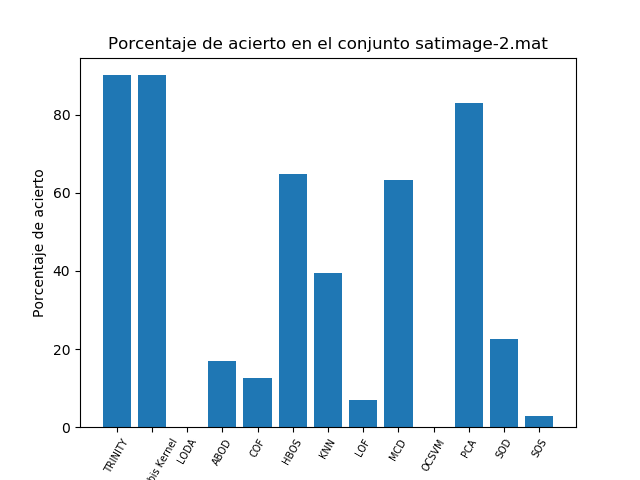
\includegraphics[scale=0.7]{imagenes/imgs-exp1/accuracy/satimage-2}
	\caption{Porcentaje de acierto sobre el conjunto de datos satimage-2}
\end{figure}

\begin{figure}[H]
	\centering
	\label{speech_accuracy}
	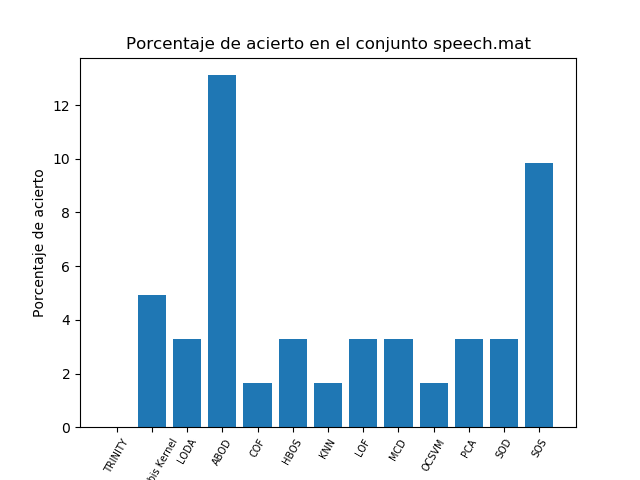
\includegraphics[scale=0.7]{imagenes/imgs-exp1/accuracy/speech}
	\caption{Porcentaje de acierto sobre el conjunto de datos speech}
\end{figure}

\begin{figure}[H]
	\centering
	\label{thyroid_accuracy}
	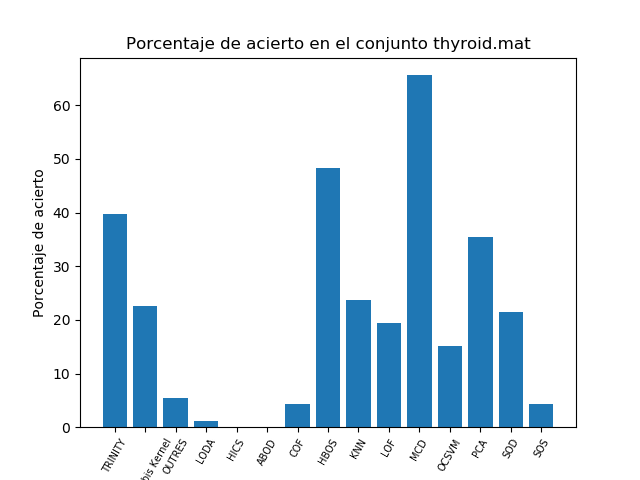
\includegraphics[scale=0.7]{imagenes/imgs-exp1/accuracy/thyroid}
	\caption{Porcentaje de acierto sobre el conjunto de datos thyroid}
\end{figure}

\begin{figure}[H]
	\centering
	\label{vertebral_accuracy}
	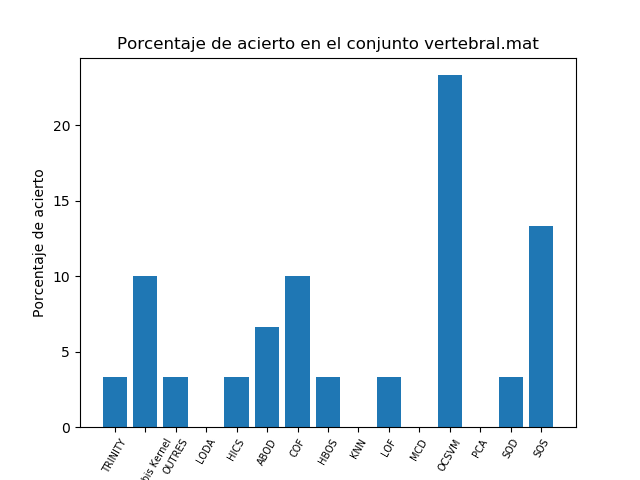
\includegraphics[scale=0.7]{imagenes/imgs-exp1/accuracy/vertebral}
	\caption{Porcentaje de acierto sobre el conjunto de datos vertebral}
\end{figure}

\begin{figure}[H]
	\centering
	\label{vowels_accuracy}
	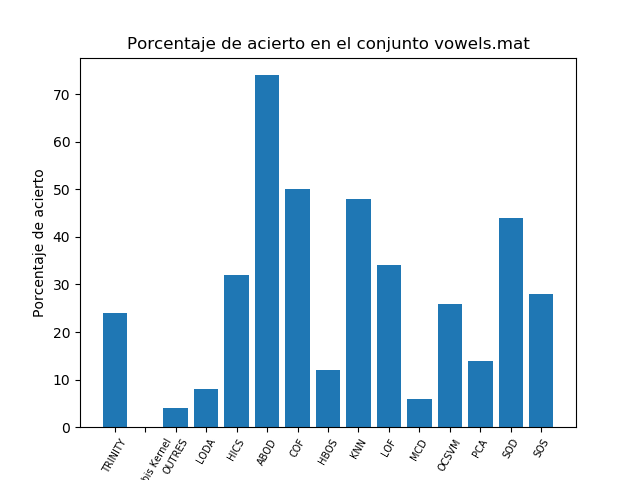
\includegraphics[scale=0.7]{imagenes/imgs-exp1/accuracy/vowels}
	\caption{Porcentaje de acierto sobre el conjunto de datos vowels}
\end{figure}

\begin{figure}[H]
	\centering
	\label{wbc_accuracy}
	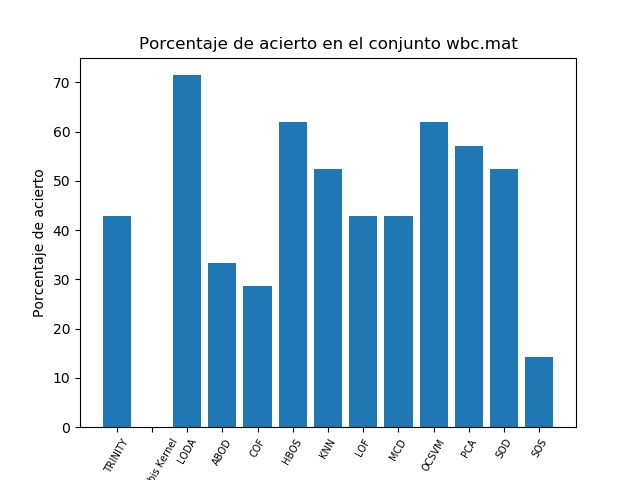
\includegraphics[scale=0.7]{imagenes/imgs-exp1/accuracy/wbc}
	\caption{Porcentaje de acierto sobre el conjunto de datos wbc}
\end{figure}

\begin{figure}[H]
	\centering
	\label{wine_accuracy}
	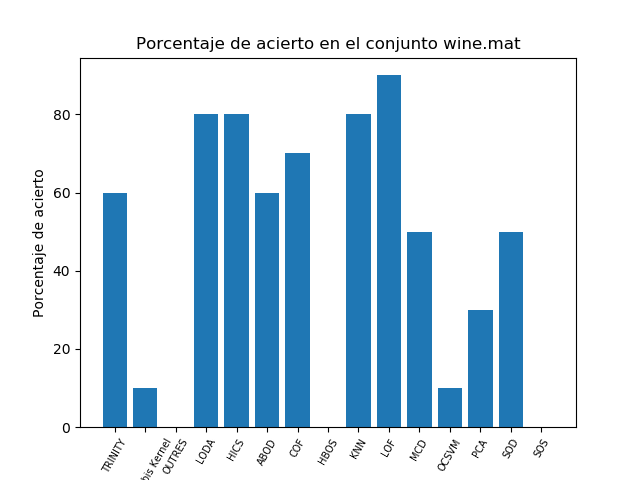
\includegraphics[scale=0.7]{imagenes/imgs-exp1/accuracy/wine}
	\caption{Porcentaje de acierto sobre el conjunto de datos wine}
\end{figure}

Como podemos observar los resultados que hemos obtenido han sido variados. En primer lugar cabe justificar algunos valores en función de la dificultad de la tarea. Como hemos comentado en la parte teórica el concepto de anomalía es algo difícil de enmarcar por lo que también es algo complejo de detectar y por tanto en función de cada conjunto de datos puede que detectemos mejor o peor sus anomalías. Por eso por ejemplo tenemos conjuntos de datos como \ref{glass_accuracy} en los que el mejor de los resultados apenas es poco más de un 20\% o \ref{optdigits_accuracy} en el que ni siquiera llegamos a dicho 20\%. Esto no es más que el reflejo de la dificultad del problema. Lo interesante de este estudio es si conseguimos mejorar en algún caso con respecto a los modelos tradicionales y la respuesta es que alguno de los modelos que hemos implementado superan en ciertos conjuntos de datos a los clásicos.

Hemos conseguido con nuestros modelos conseguir la mejor puntuación en $8$ de $22$ conjuntos de datos. Este resultado puede no parecer significativo pero debemos considerar que tenemos el doble de modelos clásicos que de modelos de ensamblaje y que ni mucho menos todos los algoritmos clásicos están al mismo nivel. Además tenemos algoritmos clásicos de todos los tipos por lo que como podemos ver en algunos conjuntos de datos no funcionan todos bien pero alguno destaca y viceversa. 

Como podemos ver en los $22$ conjuntos de datos que hemos probado los dos modelos que peores resultados nos han arrojado de loa 5 implementados son HICS y OUTRES, es decir, los dos modelos basados en subespacios que hemos implementado. Esto no quiere decir que los dos modelos sean de poca relevancia. Creo que la idea del estudio por subespacio es algo razonable y que puede arrojar buenos resultados, pero quizás no hemos utilizado para estos dos algoritmos ningún conjunto de datos conveniente. Además creo que los algoritmos de subespacios presentados son un poco rígidos en esta concepción sin querer salirse de la misma. Por ejemplo HICS obtiene sobre todo según hemos  visto anomalías que no son triviales o claramente basadas en la definición de distancias. Es por esto que, aunque lo hayamos probado como un modelo sólo, pienso que es un algoritmo más idóneo para aplicarlo en conjunción con otro tipo de algoritmos. Por ejemplo sería interesante aplicar un algoritmo basado en subespacios después de aplicar Mahalanobis Kernel puesto que este modelo y Trinity son los más fiables de los 5 que hemos estudiado. Por ejemplo podemos ver que en \ref{arrhythmia_accuracy}, \ref{breastw_accuracy}, \ref{mnist_accuracy} o \ref{satimage-2_accuracy} tanto Trinity como Mahalanobis Kernel funcionan muy bien. 

Hay un dato bastante interesante en la comparativa entre Mahalanobis Kernel y Trinity. Como hemos visto en la explicación de los modelos Trinity tiene a Mahalanobis Kernel en el primer componente. Esto en los resultados se refleja en que Trinity en general obtiene mejores resultados que Mahalanobis Kernel. El segundo componente vimos que era KNN, comparando con este modelo vemos que los resultados que obtiene Trinity son al menos iguales aunque en varios conjuntos son mejores los de Trinity que los de KNN. Por último el tercer componente de Trinity es IForest que no ha entrado dentro de esta comparativa por ser un modelo de ensamblaje también y por tanto carece de sentido contraponerlo con nuestros modelos. Esto nos está mostrando que efectivamente la combinación de modelos hace que los resultados sean más robustos obteniendo mejores resultados en general o en el peor caso manteniendo aproximadamente los resultados del modelo individual.

Por último podemos ver que LODA en general no tiene unos resultados muy espectaculares. Aún así consigue ponerse en cabeza en \ref{breastw_accuracy}, \ref{cardio_accuracy}, \ref{mammography_accuracy}, \ref{pima_accuracy} y \ref{wbc_accuracy}. En el resto de conjuntos de datos no obtiene unos buenos resultados, lo que nos está diciendo que funciona muy bien en conjuntos de datos adecuados.

Vamos a ver ambos conjuntos de datos para comprobar la razón de este comportamiento.

\begin{figure}[H]
	\centering
	\label{breastw}
	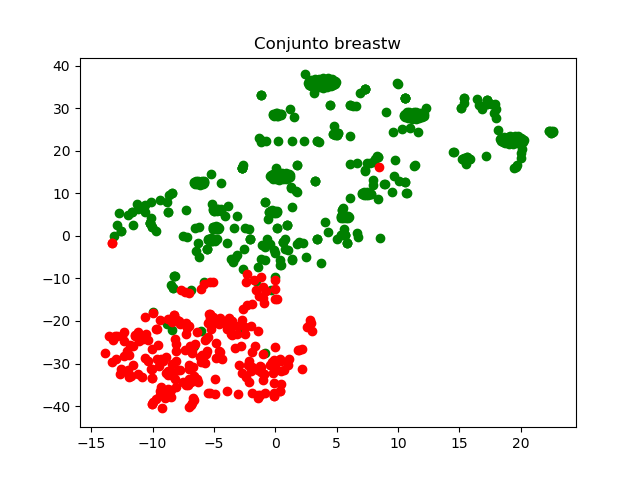
\includegraphics[scale=0.7]{imagenes/breastw}
	\caption{Proyección de breastw}
\end{figure}

\begin{figure}[H]
	\centering
	\label{glass}
	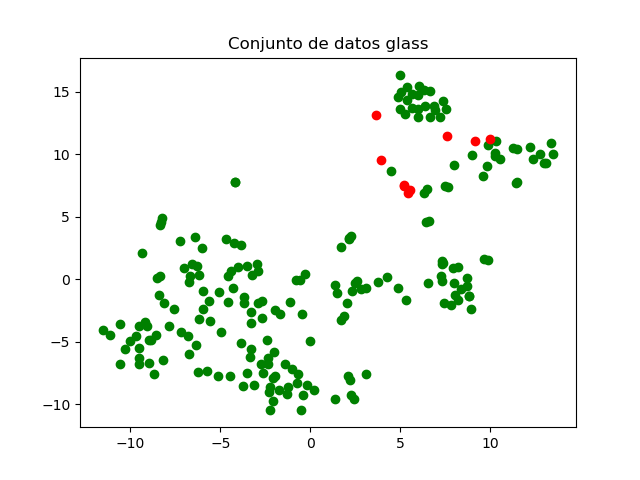
\includegraphics[scale=0.7]{imagenes/glass}
	\caption{Proyección de glass}
\end{figure}

Como podemos ver en las figuras primeras LODA funciona muy bien sobre el conjunto de datos breastw y muy mal sobre el conjunto de datos glass. Para comprobar la forma de estos dos conjuntos de datos hemos dibujado la proyección en dos dimensiones utilizando la técnica TSNE. Como podemos observar en el conjunto de datos breastw tenemos las anomalías muy separadas del resto de los datos (siendo las anomalías los datos en rojo) mientras que en glass están dentro de los datos que consideraríamos normales. Esto nos está diciendo que cuanto mayor sea la aparición de anomalías del tipo basadas en distancias mejor es el desempeño de LODA. 

Como podemos ver casi todos los modelos fallan en conjuntos de datos como optdigits. Veamos su proyección para intentar entenderlo.

\begin{figure}[H]
	\centering
	\label{optdigits}
	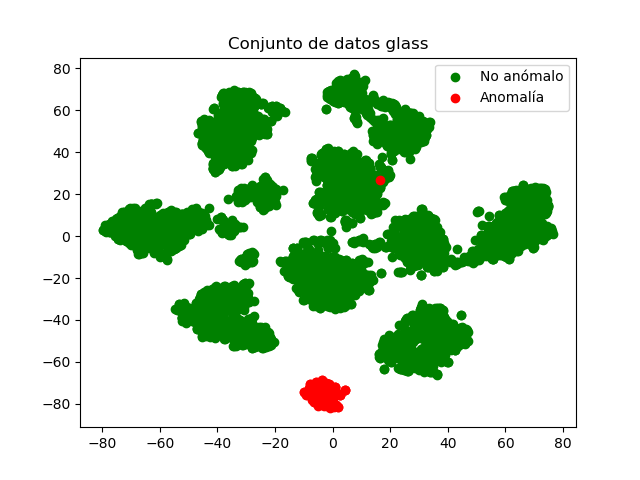
\includegraphics[scale=0.7]{imagenes/optdigits}
	\caption{Proyección de optdigits}
\end{figure}

Podría parecer que el mal desempeño de los algoritmos sea completamente ilógico al ver que las anomalías están completamente diferenciadas de los datos. Como podemos ver no sólo están separadas del resto de los datos, si no que además están muy apiñadas entre sí. Esto es un inconveniente tremendo en la detección de anomalías. Como vimos en la primera de las definiciones las anomalías deben ser datos cuya distancia al centroide sea alta cosa que no pasa en este conjuntos de datos. Si nos fijamos en la segunda definición estamos intentando estudiar la densidad de datos para ver la anomalía pero este clúster tiene una alta densidad con lo que los datos no entrarían en la definición. Este conjunto de datos refleja perfectamente la complejidad del problema. Tenemos empíricamente determinadas las anomalías pero no entran claramente en las definiciones que podemos proveer de las mismas con lo que nos es difícil clasificarlas.

HICS tiene un desempeño razonablemente bueno en el conjunto de datos wine con lo que vamos a ver su proyección e intentar sacar conclusiones.

\begin{figure}[H]
	\centering
	\label{wine}
	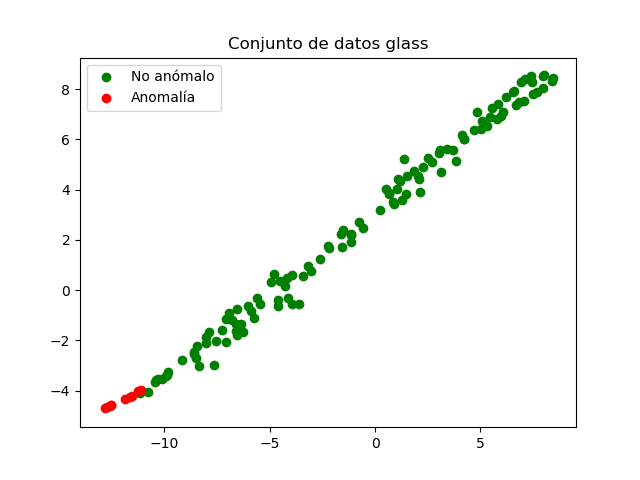
\includegraphics[scale=0.7]{imagenes/wine}
	\caption{Proyección de wine}
\end{figure}

La proyección nos está mostrando que los datos están esparcidos a lo largo de un eje con lo que podemos explicar perfectamente también el buen desempeño de Mahalanobis Kernel. En concreto podemos deducir que HICS entiende que estos datos son anómalos o al menos más anómalos que el resto de los datos porque tienen una menor densidad en su entorno. Claramente es el punto en el que menos datos hay alrededor por lo que podemos ver razonable el comportamiento satisfactorio de HICS.

Para comprender el comportamiento de OUTRES es buena idea comprobar no sólo cuándo tenemos buenos resultados, si no que además por el propio algoritmo podemos ver el subespacio de los datos en el que cada dato es anómalo.

OUTRES no obtiene demasiados resultados satisfactorios pero donde mejor funciona es en breastw y en pima. Ya hemos visto cómo es la proyección de breastw, veamos la de pima.

\begin{figure}[H]
	\centering
	\label{pima}
	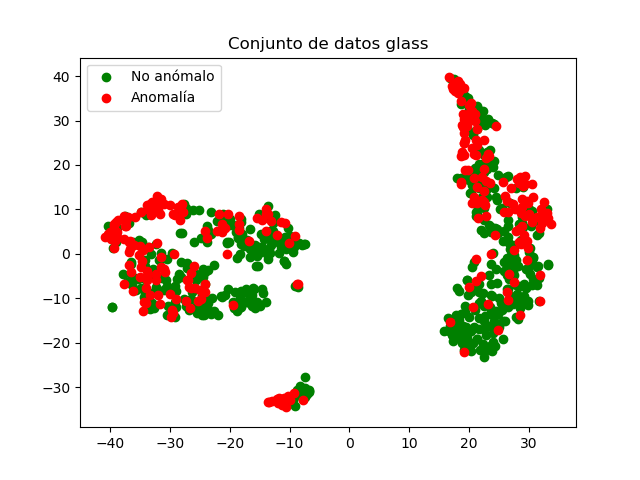
\includegraphics[scale=0.7]{imagenes/pima}
	\caption{Proyección de pima}
\end{figure}

En un primer vistazo este conjunto de datos parece bastante complejo para obtener buenos resultados, por lo que merece la pena que veamos algunos de los subespacios en los que las instancias son anómalas para así poder entender un poco mejor el resultado. Estas imágenes son de todos los subespacios posibles obtenidos por OUTRES para cada instancia (en rojo) junto con el vecindario (en azul). Si tiene dimensión 2 se pintan directamente, si tienen una dimensionalidad mayor se hace primero la reducción de dimensionalidad mediante la técnica TSNE. Veamos algunos ejemplos:

\begin{figure}[H]
	\centering
	\label{22}
	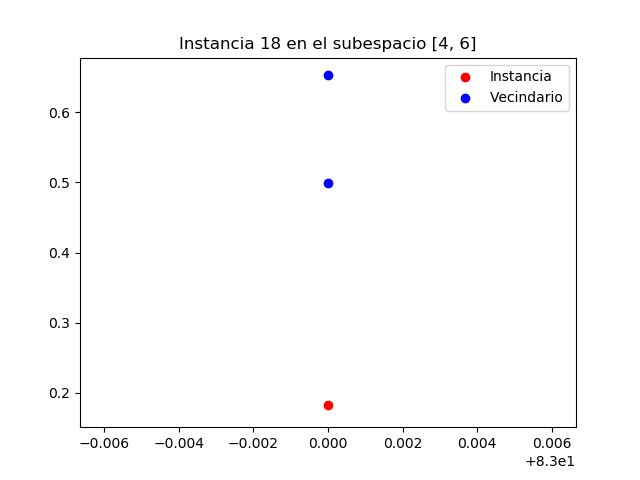
\includegraphics[scale=0.7]{imagenes/22}
	\caption{Instancia 18 sobre el subespacio $[4,6]$}
\end{figure}

Como podemos ver en dos dimensiones se comprueba rápidamente que la instancia es anómala, pero estos subespacios no son los más interesantes. Cuanto mayor es el vecindario y mayor es la dimensionalidad más conclusiones podemos obtener. Veamos uno de estos ejemplos de mayor dimensionalidad.

\begin{figure}[H]
	\centering
	\label{68_tsne}
	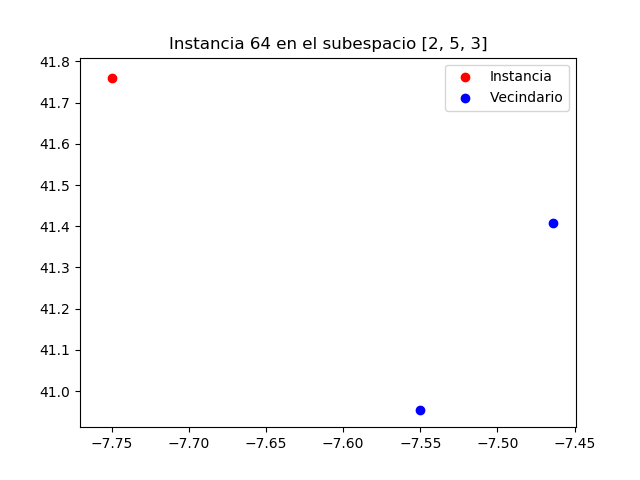
\includegraphics[scale=0.7]{imagenes/68_tsne}
	\caption{Instancia 64 sobre el subespacio $[2,5,3]$}
\end{figure}

Como podemos ver en este caso tenemos un subespacio de dimensión 3. Las instancias azules están más próximas entre sí que con respecto a la roja por lo que es normal que esta sea considerada anómala en este subespacio pues está aislada.

\begin{figure}[H]
	\centering
	\label{173_tsne}
	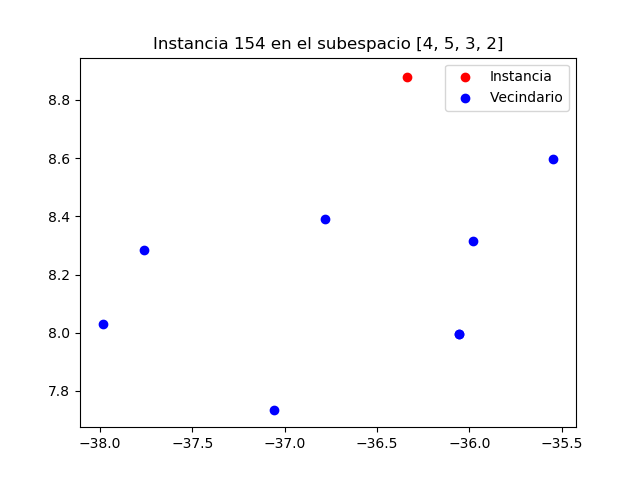
\includegraphics[scale=0.7]{imagenes/173_tsne}
	\caption{Instancia 154 sobre el subespacio $[4,5,3,2]$}
\end{figure}

Este ejemplo es de un subespacio de dimensionalidad 4. Aquí podemos ver claramente que de nuevo la instancia no sólo se encuentra algo aislada, si no que se encuentra en lo que podemos calificar como una zona poco densa con respecto a sus vecinos. Por ejemplo el dato central de esta figura no podría ser nunca considerado una anomalía en este subespacio concreto, pues al menos el vecindario sería como mínimo el que estamos observando y por tanto vemos que no es un dato raro, de hecho es el centroide de este vecindario.

\begin{figure}[H]
	\centering
	\label{190_tsne}
	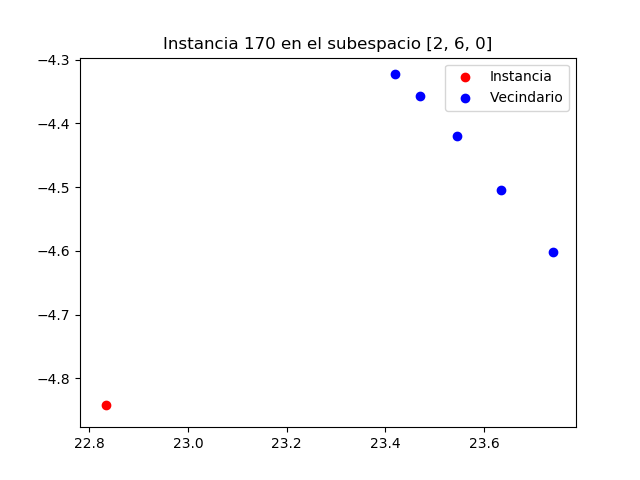
\includegraphics[scale=0.7]{imagenes/190_tsne}
	\caption{Instancia 170 sobre el subespacio $[2,6,0]$}
\end{figure}

Este ejemplo es aún más esclarecedor pues como podemos ver los datos normales están no sólo muy concentrados, si no además alineados. Esta idea de encontrar alineamiento en subespacios podría ser una buena característica a buscar en subespacios para poder emplear en ellos técnicas como Mahalanobis Kernel.

Para que sea más fácil ver los datos de acierto, vamos a ponerlos en una tabla.

% Please add the following required packages to your document preamble:
% \usepackage[normalem]{ulem}
% \useunder{\uline}{\ul}{}
\begin{table}[H]
	\resizebox{\textwidth}{!}{
	\begin{tabular}{|c|c|c|c|c|c|c|c|c|c|c|c|c|c|c|c|}
		\hline
		{\ul \textbf{Data / Mod}} & \textbf{Trinity}   & \textbf{MK}        & \textbf{OUTRES} & \textbf{LODA}      & \textbf{HICS} & \textbf{ABOD}      & \textbf{COF}       & \textbf{HBOS}      & \textbf{KNN} & \textbf{LOF}       & \textbf{MCD}       & \textbf{OCSVM}     & \textbf{PCA}       & \textbf{SOD}       & \textbf{SOS} \\ \hline
		\textbf{annthyroid}       & 26.2172\%          & 12.3595\%          & 7.4906\%        & 8.9887\%           & 6.5543\%      & 25.0936\%          & 23.0936\%          & 26.0299\%          & 28.4644\%    & 29.2134\%          & \textbf{45.8801\%} & 11.2359\%          & 23.7827\%          & 30.7116\%          & 7.4906\%     \\ \hline
		\textbf{arrhythmia}       & 48.4848\%          & \textbf{51.5151\%} & NAN             & 37.8787\%          & NAN           & 37.8787\%          & 46.9696\%          & 50\%               & 48.4848\%    & 42.4242\%          & \textbf{51.5151\%} & 15.1515\%          & 42.4242\%          & 28.7878\%          & 13.6363\%    \\ \hline
		\textbf{breastw}          & 93.3054\%          & \textbf{95.3974\%} & 50.6276\%       & \textbf{95.3974}   & 1.2552\%      & NAN                & 8.3682\%           & 93.7238\%          & 91.2133\%    & 13.3891\%          & 89.9581\%          & 91.2133\%          & 92.8870\%          & 80.7531\%          & 49.7907\%    \\ \hline
		\textbf{cardio}           & 44.3181\%          & 51.7045\%          & NAN             & 59.0909\%          & NAN           & 22.7272\%          & 19.8863\%          & 47.1590\%          & 33.5227\%    & 17.0454\%          & 40.9090\%          & 50.5681\%          & \textbf{60.7954\%} & 25.5681\%          & 10.7954\%    \\ \hline
		\textbf{glass}            & 11.1111\%          & 0\%                & 0\%             & 0\%                & 11.1111\%     & 11.1111\%          & \textbf{22.2222\%} & 0\%                & 11.1111\%    & \textbf{22.2222\%} & 0\%                & 11.1111\%          & 11.1111\%          & \textbf{22.2222\%} & 11.1111\%    \\ \hline
		\textbf{ionosphere}       & 73.0158\%          & 57.1428\%          & NAN             & 46.8253\%          & NAN           & 84.1269\%          & 77.7777\%          & 48.4126\%          & 87.3015\%    & 76.1904\%          & \textbf{88.0952\%} & 64.2857\%          & 59.5238\%          & 80.1587\%          & 61.1111\%    \\ \hline
		\textbf{letter}           & 16\%               & 15\%               & NAN             & 4\%                & NAN           & NAN                & 42\%               & 6\%                & 43\%         & 46\%               & 16\%               & 48\%               & 8\%                & \textbf{51\%}      & 6\%          \\ \hline
		\textbf{lympho}           & 83.3333\%          & 50\%               & NAN             & 0\%                & NAN           & 33.3333\%          & 50\%               & \textbf{100\%}     & 66.6666\%    & 83.3333\%          & 50\%               & 50\%               & 66.6666\%          & 50\%               & 16.6666\%    \\ \hline
		\textbf{mammography}      & 25.7692\%          & 1.1538\%           & 5.3846\%        & \textbf{28.0769\%} & 8.0769\%      & 0.3846\%           & 13.8461\%          & 12.6923\%          & 21.9230\%    & 19.2307\%          & 0.7692\%           & 27.3076\%          & 25.7692\%          & 15\%               & 5\%          \\ \hline
		\textbf{mnist}            & 40.2857\%          & \textbf{54.7142\%} & NAN             & 2\%                & NAN           & 28.5714\%          & 21.4285\%          & 17.1428\%          & 39.5714\%    & 24.2857\%          & 49.1428\%          & 0.1428\%           & 38.5714\%          & 20.5714\%          & 11.5714\%    \\ \hline
		\textbf{musk}             & 34.0206\%          & 0\%                & NAN             & 32.9896\%          & NAN           & 2.0618\%           & 8.2474\%           & 90.7216\%          & 1.0309\%     & 3.0927\%           & 96.9072\%          & 0\%                & \textbf{98.9690\%} & 4.1237\%           & 6.1855\%     \\ \hline
		\textbf{optdigits}        & 1.3333\%           & 0\%                & NAN             & 0\%                & NAN           & 4.6666\%           & 9.3333\%           & \textbf{18.6666\%} & 3.3333\%     & 10.6666\%          & 0\%                & 1.3333\%           & 0\%                & 3.3333\%           & 2.6666\%     \\ \hline
		\textbf{pendigits}        & 25\%               & 16.6666\%          & 2.5641\%        & 0\%                & NAN           & 7.0512\%           & 7.6923\%           & 32.0512\%          & 8.9743\%     & 6.4102\%           & 10.2564\%          & 26.2820\%          & \textbf{32.6923\%} & 6.4102\%           & 2.5641\%     \\ \hline
		\textbf{pima}             & 50.7462\%          & 38.8059\%          & 34.7014\%       & \textbf{54.8507\%} & 30.5970\%     & 45.8955\%          & 37.3134\%          & 50.7462\%          & 48.1343\%    & 36.9402\%          & 51.4925\%          & 39.5522\%          & 49.6268\%          & 41.4179\%          & 36.1940\%    \\ \hline
		\textbf{satellite}        & 54.3713\%          & 32.8585\%          & NAN             & 12.6227\%          & NAN           & NAN                & 43.5166\%          & 56.8271\%          & 50.0982\%    & 37.0825\%          & \textbf{68.4675\%} & 30.1571\%          & 48.3791\%          & 41.3064\%          & 29.9115\%    \\ \hline
		\textbf{satimage-2}       & \textbf{90.1408\%} & \textbf{90.1408\%} & NAN             & 0\%                & NAN           & 16.9014\%          & 12.6760\%          & 64.7887\%          & 39.4366\%    & 7.0422\%           & 63.3802\%          & 0\%                & 83.0985\%          & 22.5352\%          & 2.8169\%     \\ \hline
		\textbf{speech}           & 0\%                & 4.9180\%           & NAN             & 3.2786\%           & NAN           & \textbf{13.1147\%} & 1.6393\%           & 3.2786\%           & 1.6393\%     & 3.2786\%           & 3.2786\%           & 1.6393\%           & 3.2786\%           & 3.2786\%           & 9.8360\%     \\ \hline
		\textbf{thyroid}          & 39.7849\%          & 22.5806\%          & 5.3763\%        & 1.0752\%           & 0\%           & 0\%                & 4.3010\%           & 48.3870\%          & 23.6559\%    & 19.3548\%          & \textbf{65.5913\%} & 15.0537\%          & 35.4838\%          & 21.5053\%          & 4.3010\%     \\ \hline
		\textbf{vertebral}        & 3.3333\%           & 10\%               & 3.3333\%        & 0\%                & 3.3333\%      & 6.6666\%           & 10\%               & 3.3333\%           & 0\%          & 3.3333\%           & 0\%                & \textbf{23.3333\%} & 0\%                & 3.3333\%           & 13.3333\%    \\ \hline
		\textbf{vowels}           & 24\%               & 0\%                & 4\%             & 8\%                & 32\%          & \textbf{74\%}      & 50\%               & 12\%               & 48\%         & 34\%               & 6\%                & 26\%               & 14\%               & 44\%               & 28\%         \\ \hline
		\textbf{wbc}              & 42.8571\%          & 0\%                & NAN             & \textbf{71.4285\%} & NAN           & 33.3333\%          & 28.5714\%          & 61.9047\%          & 52.3809\%    & 42.8571\%          & 42.8571\%          & 61.9047\%          & 57.1428\%          & 52.3809\%          & 14.2857\%    \\ \hline
		\textbf{wine}             & 60\%               & 10\%               & 0\%             & 80\%               & 80\%          & 60\%               & 70\%               & 0\%                & 80\%         & \textbf{90\%}      & 50\%               & 10\%               & 30\%               & 50\%               & 0\%          \\ \hline
	\end{tabular}
}
\end{table}

Ahora para completar vamos a ver las gráficas de los tiempos consumidos por cada algoritmo para cada conjunto de datos junto con la tabla de los mismos.

\begin{figure}[H]
	\centering
	\label{annthyroid_times}
	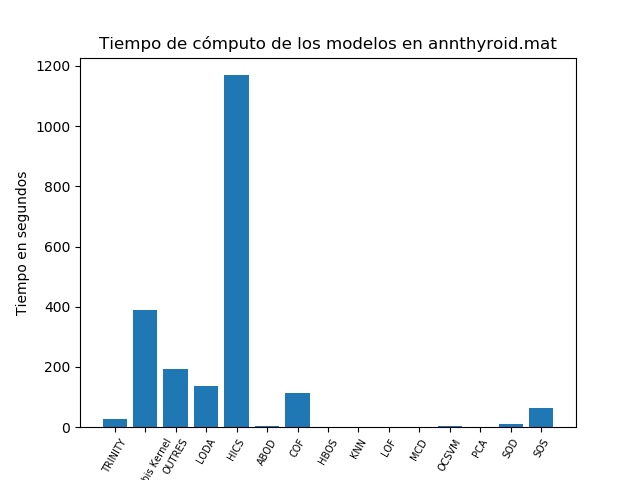
\includegraphics[scale=0.7]{imagenes/imgs-exp1/times/annthyroid}
	\caption{Tiempos sobre el conjunto de datos annthyroid}
\end{figure}

\begin{figure}[H]
	\centering
	\label{arrhythmia_times}
	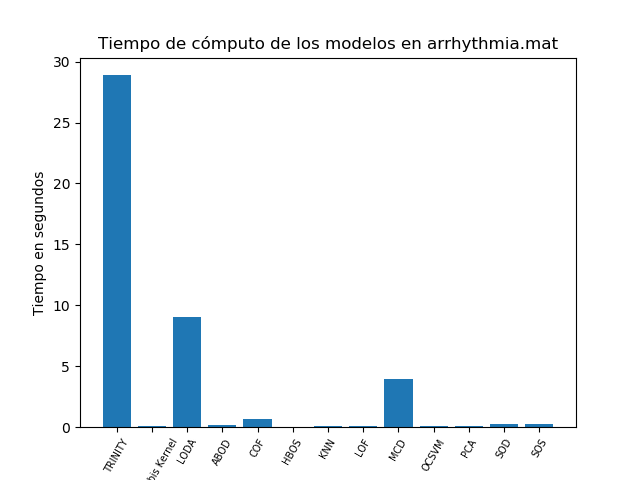
\includegraphics[scale=0.7]{imagenes/imgs-exp1/times/arrhythmia}
	\caption{Tiempos sobre el conjunto de datos arrhythmia}
\end{figure}

\begin{figure}[H]
	\centering
	\label{breastw_times}
	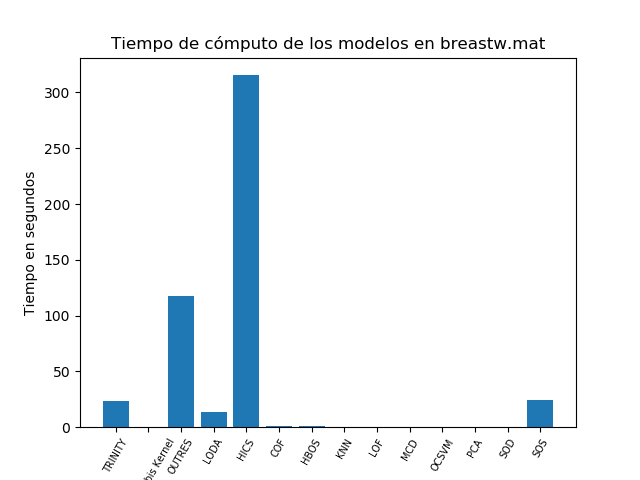
\includegraphics[scale=0.7]{imagenes/imgs-exp1/times/breastw}
	\caption{Tiempos sobre el conjunto de datos breastw}
\end{figure}

\begin{figure}[H]
	\centering
	\label{cardio_times}
	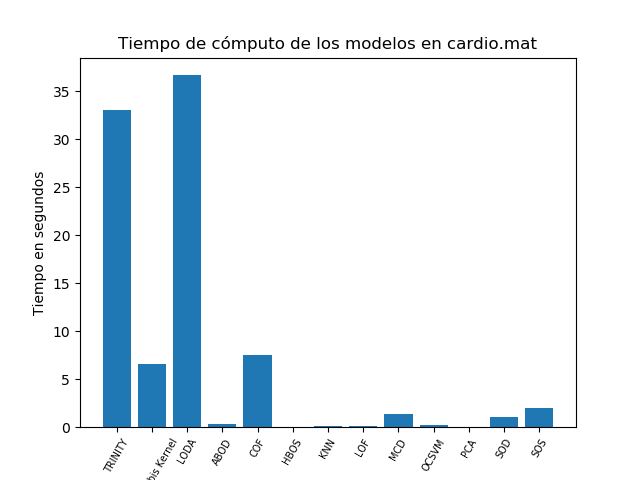
\includegraphics[scale=0.7]{imagenes/imgs-exp1/times/cardio}
	\caption{Tiempos sobre el conjunto de datos cardio}
\end{figure}

\begin{figure}[H]
	\centering
	\label{glass_times}
	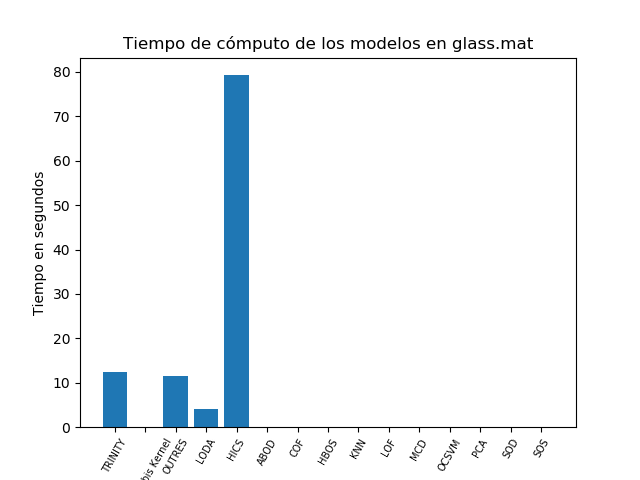
\includegraphics[scale=0.7]{imagenes/imgs-exp1/times/glass}
	\caption{Tiempos sobre el conjunto de datos glass}
\end{figure}

\begin{figure}[H]
	\centering
	\label{ionosphere_times}
	\includegraphics[scale=0.7]{imagenes/imgs-exp1/times/ionosphere}
	\caption{Tiempos sobre el conjunto de datos ionosphere}
\end{figure}

\begin{figure}[H]
	\centering
	\label{letter_times}
	\includegraphics[scale=0.7]{imagenes/imgs-exp1/times/letter}
	\caption{Tiempos sobre el conjunto de datos letter}
\end{figure}

\begin{figure}[H]
	\centering
	\label{lympho_times}
	\includegraphics[scale=0.7]{imagenes/imgs-exp1/times/lympho}
	\caption{Tiempos sobre el conjunto de datos lympho}
\end{figure}

\begin{figure}[H]
	\centering
	\label{mammography_times}
	\includegraphics[scale=0.7]{imagenes/imgs-exp1/times/mammography}
	\caption{Tiempos sobre el conjunto de datos mammography}
\end{figure}

\begin{figure}[H]
	\centering
	\label{mnist_times}
	\includegraphics[scale=0.7]{imagenes/imgs-exp1/times/mnist}
	\caption{Tiempos sobre el conjunto de datos mnist}
\end{figure}

\begin{figure}[H]
	\centering
	\label{musk_times}
	\includegraphics[scale=0.7]{imagenes/imgs-exp1/times/musk}
	\caption{Tiempos sobre el conjunto de datos musk}
\end{figure}

\begin{figure}[H]
	\centering
	\label{optdigits_times}
	\includegraphics[scale=0.7]{imagenes/imgs-exp1/times/optdigits}
	\caption{Tiempos sobre el conjunto de datos optdigits}
\end{figure}

\begin{figure}[H]
	\centering
	\label{pendigits_times}
	\includegraphics[scale=0.7]{imagenes/imgs-exp1/times/pendigits}
	\caption{Tiempos sobre el conjunto de datos pendigits}
\end{figure}

\begin{figure}[H]
	\centering
	\label{pima_times}
	\includegraphics[scale=0.7]{imagenes/imgs-exp1/times/pima}
	\caption{Tiempos sobre el conjunto de datos pima}
\end{figure}

\begin{figure}[H]
	\centering
	\label{satellite_times}
	\includegraphics[scale=0.7]{imagenes/imgs-exp1/times/satellite}
	\caption{Tiempos sobre el conjunto de datos satellite}
\end{figure}

\begin{figure}[H]
	\centering
	\label{satimage-2_times}
	\includegraphics[scale=0.7]{imagenes/imgs-exp1/times/satimage-2}
	\caption{Tiempos sobre el conjunto de datos satimage-2}
\end{figure}

\begin{figure}[H]
	\centering
	\label{speech_times}
	\includegraphics[scale=0.7]{imagenes/imgs-exp1/times/speech}
	\caption{Tiempos sobre el conjunto de datos speech}
\end{figure}

\begin{figure}[H]
	\centering
	\label{thyroid_times}
	\includegraphics[scale=0.7]{imagenes/imgs-exp1/times/thyroid}
	\caption{Tiempos sobre el conjunto de datos thyroid}
\end{figure}

\begin{figure}[H]
	\centering
	\label{vertebral_times}
	\includegraphics[scale=0.7]{imagenes/imgs-exp1/times/vertebral}
	\caption{Tiempos sobre el conjunto de datos vertebral}
\end{figure}

\begin{figure}[H]
	\centering
	\label{vowels_times}
	\includegraphics[scale=0.7]{imagenes/imgs-exp1/times/vowels}
	\caption{Tiempos sobre el conjunto de datos vowels}
\end{figure}

\begin{figure}[H]
	\centering
	\label{wbc_times}
	\includegraphics[scale=0.7]{imagenes/imgs-exp1/times/wbc}
	\caption{Tiempos sobre el conjunto de datos wbc}
\end{figure}

\begin{figure}[H]
	\centering
	\label{wine_times}
	\includegraphics[scale=0.7]{imagenes/imgs-exp1/times/wine}
	\caption{Tiempos sobre el conjunto de datos wine}
\end{figure}

Hay una cosa que podemos ver claramente y es el hecho de que los algoritmos de ensamblaje consumen un tiempo mayor en general que los algoritmos clásicos. De entre los 5 algoritmos implementados que se han propuesto podemos ver que cuando OUTRES y HICS se ejecutan sobre el conjunto son los que consumen un mayor tiempo, siendo no sólo los que más tiempo consumen si no que además obtienen los mayores tiempos de todos los conjuntos de datos superando incluso los mil segundos.

Tanto Trinity como Mahalanobis Kernel y LODA tienen conjuntos de datos en los que son los algoritmos que más tardan por lo que no podemos decir que uno sea más lento que el resto. 

Veamos los tiempos en una tabla de datos.

% Please add the following required packages to your document preamble:
% \usepackage[normalem]{ulem}
% \useunder{\uline}{\ul}{}
\begin{table}[H]
\resizebox{\textwidth}{!}{
	\begin{tabular}{|c|c|c|c|c|c|c|c|c|c|c|c|c|c|c|c|}
		\hline
		{\ul \textbf{Data / Mod}} & \textbf{Trinity} & \textbf{MK}   & \textbf{OUTRES} & \textbf{LODA} & \textbf{HICS} & \textbf{ABOD} & \textbf{COF} & \textbf{HBOS} & \textbf{KNN} & \textbf{LOF} & \textbf{MCD} & \textbf{OCSVM} & \textbf{PCA} & \textbf{SOD} & \textbf{SOS}  \\ \hline
		\textbf{annthyroid}       & 28.5212 seg      & 390.5937 seg  & 193.6110 seg    & 137.8692 seg  & 1169.3422 seg & 2.5419 seg    & 114.7065 seg & 1.2222 seg    & 0.2307 seg   & 0.1145 seg   & 1.5861 seg   & 2.6132 seg     & 0.0038 seg   & 10.9631 seg  & 63.2884 seg   \\ \hline
		\textbf{arrhythmia}       & 28.8828 seg      & 0.1243 seg    & NAN             & 9.0474 seg    & NAN           & 0.1662 seg    & 0.6819 seg   & 0.0508 seg    & 0.0759 seg   & 0.0917 seg   & 3.9257 seg   & 0.1281 seg     & 0.0843 seg   & 0.2299 seg   & 0.2713 seg    \\ \hline
		\textbf{breastw}          & 23.3296 seg      & 0.3165 seg    & 117.8225 seg    & 13.2879 seg   & 315.4130 seg  & NAN           & 1.0530 seg   & 0.7055 seg    & 0.0057 seg   & 0.0098 seg   & 0.5311 seg   & 0.0200 seg     & 0.0189 seg   & 0.2007 seg   & 23.9622 seg   \\ \hline
		\textbf{cardio}           & 33.0496 seg      & 6.5851 seg    & NAN             & 36.6768 seg   & NAN           & 0.3701 seg    & 7.4887 seg   & 0.0053 seg    & 0.0872 seg   & 0.1170 seg   & 1.3748 seg   & 0.2028 seg     & 0.0051 seg   & 1.0434 seg   & 2.0196 seg    \\ \hline
		\textbf{glass}            & 12.5272 seg      & 0.0220 seg    & 11.5349 seg     & 4.0798 seg    & 79.2560 seg   & 0.0358 seg    & 0.1341 seg   & 0.0036 seg    & 0.0014 seg   & 0.0021 seg   & 0.0905 seg   & 0.0028 seg     & 0.0021 seg   & 0.0421 seg   & 0.1425 seg    \\ \hline
		\textbf{ionosphere}       & 16.5319 seg      & 0.0565 seg    & NAN             & 6.9664 seg    & NAN           & 0.0641 seg    & 0.3415 seg   & 0.0062 seg    & 0.0071 seg   & 0.0101 seg   & 0.9893 seg   & 0.0103 seg     & 0.0044 seg   & 0.0897 seg   & 0.2140 seg    \\ \hline
		\textbf{letter}           & 41.8301 seg      & 5.1648 seg    & NAN             & 31.8875 seg   & NAN           & NAN           & 5.1220 seg   & 0.0075 seg    & 0.0839 seg   & 0.1047 seg   & 13.1818 seg  & 0.2577 seg     & 0.0073 seg   & 0.8809 seg   & 25.3305 seg   \\ \hline
		\textbf{lympho}           & 12.2874 seg      & 0.0187 seg    & NAN             & 2.8804 seg    & NAN           & 0.0228 seg    & 0.0693 seg   & 0.0038 seg    & 0.0014 seg   & 0.0017 seg   & 0.1741 seg   & 0.0020 seg     & 0.0029 seg   & 0.0288 seg   & 0.0526 seg    \\ \hline
		\textbf{mammography}      & 31.5619 seg      & 1444.1323 seg & 27765.1978 seg  & 224.8207 seg  & 2502.0258 seg & 1.7394 seg    & 280.7073 seg & 0.0037 seg    & 0.2790 seg   & 0.3027 seg   & 2.3683 seg   & 5.8535 seg     & 0.0066 seg   & 25.2311 seg  & 9653.7372 seg \\ \hline
		\textbf{mnist}            & 42.7623 seg      & 464.8962 seg  & NAN             & 150.1434 seg  & NAN           & 16.4729 seg   & 154.4384 seg & 0.0502 seg    & 9.7564 seg   & 10.2119 seg  & 37.5253 seg  & 14.0057 seg    & 0.1746 seg   & 22.8423 seg  & 34.5968 seg   \\ \hline
		\textbf{musk}             & 42.8683 seg      & 34.4336 seg   & NAN             & 60.4207 seg   & NAN           & 1.6461 seg    & 23.2048 seg  & 0.0555 seg    & 1.1578 seg   & 1.3294 seg   & 121.9505 seg & 4.1720 seg     & 0.2416 seg   & 3.8690 seg   & 5.7815 seg    \\ \hline
		\textbf{optdigits}        & 36.2723 seg      & 145.6876 seg  & NAN             & 103.9115 seg  & NAN           & 6.6622 seg    & 47.9141 seg  & 0.0312 seg    & 2.3891 seg   & 2.4586 seg   & 29.2400 seg  & 6.0881 seg     & 0.0513 seg   & 8.8440 seg   & 12.5010 seg   \\ \hline
		\textbf{pendigits}        & 34.0999 seg      & 340.2855 seg  & 2757.0345 seg   & 135.0839 seg  & NAN           & 1.4151 seg    & 75.1194 seg  & 0.0076 seg    & 0.3140 seg   & 0.4336 seg   & 6.3704 seg   & 3.1717 seg     & 0.0105 seg   & 10.5999 seg  & 25.3345 seg   \\ \hline
		\textbf{pima}             & 26.3576 seg      & 0.3482 seg    & 40.6379 seg     & 15.2128 seg   & 150.1283 seg  & 0.1230 seg    & 0.9667 seg   & 0.0021 seg    & 0.0053 seg   & 0.0057 seg   & 0.5652 seg   & 0.0567 seg     & 0.0028 seg   & 0.2303 seg   & 0.4855 seg    \\ \hline
		\textbf{satellite}        & 48.2618 seg      & 301.9960 seg  & NAN             & 129.6712 seg  & NAN           & NAN           & 70.0058 seg  & 0.0146 seg    & 0.7749 seg   & 0.8185 seg   & 38.1214 seg  & 6.5430 seg     & 0.0305 seg   & 9.8771 seg   & 21.9062 seg   \\ \hline
		\textbf{satimage-2}       & 39.7535 seg      & 200.5037 seg  & NAN             & 113.2818 seg  & NAN           & 1.7584 seg    & 54.0372 seg  & 0.0139 seg    & 0.7183 seg   & 0.7796 seg   & 32.5359 seg  & 5.4775 seg     & 0.0240 seg   & 8.2761 seg   & 15.4193 seg   \\ \hline
		\textbf{speech}           & 76.6633 seg      & 62.2470 seg   & NAN             & 73.0844 seg   & NAN           & 13.2967 seg   & 58.9203 seg  & 0.1523 seg    & 8.6546 seg   & 8.4023 seg   & 143.7647 seg & 7.8068 seg     & 0.5699 seg   & 12.2820 seg  & 7.1908 seg    \\ \hline
		\textbf{thyroid}          & 32.6503 seg      & 65.3469 seg   & 64.2370 seg     & 72.1607 seg   & 376.2697 seg  & 0.5982 seg    & 21.8574 seg  & 0.0022 seg    & 0.0450 seg   & 0.0676 seg   & 1.0717 seg   & 0.5607 seg     & 0.0026 seg   & 3.3138 seg   & 29.4608 seg   \\ \hline
		\textbf{vertebral}        & 13.4726 seg      & 0.0301 seg    & 1.7653 seg      & 4.6250 seg    & 9.1404 seg    & 0.0395 seg    & 0.1153 seg   & 0.0013 seg    & 0.0015 seg   & 0.0019 seg   & 0.0435 seg   & 0.0050 seg     & 0.0011 seg   & 0.0472 seg   & 0.1450 seg    \\ \hline
		\textbf{vowels}           & 36.2093 seg      & 3.1876 seg    & 426.6157 seg    & 28.2930 seg   & 5126.5627 seg & 0.2367 seg    & 3.3253 seg   & 0.0030 seg    & 0.0247 seg   & 0.0346 seg   & 0.8870 seg   & 0.0890 seg     & 0.0023 seg   & 0.6860 seg   & 1.3831 seg    \\ \hline
		\textbf{wbc}              & 17.0011 seg      & 0.0675 seg    & NAN             & 7.5109 seg    & NAN           & 0.0700 seg    & 0.2526 seg   & 0.0061 seg    & 0.0082 seg   & 0.0080 seg   & 1.7926 seg   & 0.0101 seg     & 0.0043 seg   & 0.0964 seg   & 0.2449 seg    \\ \hline
		\textbf{wine}             & 11.2756 seg      & 0.0165 seg    & 58.9642 seg     & 2.4540 seg    & 774.9212 seg  & 0.0231 seg    & 0.0421 seg   & 0.0025 seg    & 0.0010 seg   & 0.0032 seg   & 0.1075 seg   & 0.0020 seg     & 0.0020 seg   & 0.0226 seg   & 0.0539 seg    \\ \hline
	\end{tabular}
}
\end{table}

\section{Conclusiones y trabajo futuro}

Ya hemos visto todos los resultados que hemos obtenido con los modelos y el análisis de cómo funcionan de forma teórica por lo que hemos reunido todos los ingredientes necesarios para sacar algunas conclusiones sobre este estudio.

En primer lugar cabe decir que en general los algoritmos que hemos implementado (salvo los basados en subespacios) están al mismo nivel de rendimiento que los modelos clásicos. En este estudio he comprendido el potencial que podría tener un buen modelo que combine de forma adecuada modelos clásicos o incluso modelos de ensamblaje.

El enfoque de los algoritmos basados en subespacios que se han implementado no parece ser algo que funcione en conjuntos de datos reales aunque los conceptos de densidad puedan resultar interesantes por ofrecer otro punto de vista. Algoritmos como HICS y OUTRES pueden ofrecer un buen aporte extra para un modelo ya implementado, es decir, utilizar estos algoritmos para detectar lo que ellos mismos llaman anomalías no triviales. Como modelos individuales ya hemos visto que no tienen un desempeño demasiado bueno además del alto consumo en tiempo que tienen y que hace que sea difícil su aplicación en conjuntos de datos más grandes. 

Un punto de vista interesante y que se debería tener en cuenta es la aplicación de modelos en función del tipo de datos que tengamos. Es decir, un algoritmo que regule su propio comportamiento primero analizando brevemente el conjunto de datos con algunos parámetros y posteriormente ejecutando los métodos que convengan. 

Hemos podido ver en los resultados que para todos los modelos existen conjuntos de datos en los que no funcionan bien, incluso algunos llegan a sacar un 0\% tanto de los clásicos como de los algoritmos de ensamblaje. Esto nos está reflejando que no es una aproximación inteligente intentar dar un algoritmo que aplique una misma técnica para todos los conjuntos de datos con los que se encuentre.

Creo que los resultados que hemos obtenido dejan margen de mejora, lo cual hace este campo interesante y desafiante para proponer nuevas ideas sobre la mesa. En primer lugar hemos visto que todos los algoritmos tienen problemas en cuanto al manejo de los valores perdidos. Es lógico que estos algoritmos no estén preparados ante vectores que no dispongan de ningún valor numérico, pero creo que sería interesante disponer de alguna técnica que nos permita trabajar con vectores que tengan algunos valores no disponibles. Podríamos pensar por ejemplo en alguna técnica que considere la proyección del conjunto de datos sobre los atributos disponibles de esa instancia con valores perdido y hacer un estudio sobre esa proyección. Como hemos discutido previamente es fácil que, tras esas instancias con valores perdidos, se escondan anomalías reales. 

Los algoritmos como HICS y OUTRES tienen ideas teóricas muy elaboradas pero no piensan en los problemas de eficiencia que llevan tras de sí, con lo que se hacen algoritmos poco prácticos para su uso. Sería de utilidad la inclusión de técnicas inherentes a los algoritmos que mejoren su eficiencia sin reducir en exceso su desempeño. Por ejemplo la aproximación de HICS al obtener los subespacios de alto contraste siempre se queda con los de mayor contraste pero a cambio debemos hacer un cómputo desmesurado de subespacios y contrastes que disminuyen terriblemente su eficiencia.

Por contra hemos visto como Trinity consigue unos resultados robustos en comparación con los modelos que emplea. Este tipo de algoritmos de ensamblaje pueden tener mejores resultados según la experiencia que he desarrollado en este trabajo. Creo que se podrían mezclar diferentes técnicas en un algoritmo como Trinity. Por ejemplo hemos visto que hay subespacios o trozos de los conjuntos de datos en los que el alineamiento de las instancias en hiperplanos u otras formas es clara y evidente. Esto nos hace pensar en la posibilidad de usar en dichas circunstancias algoritmos como Mahalanobis Kernel. 

Todo este análisis nos está dejando claro que el futuro de los algoritmos de ensamblaje es prometedor y como línea principal de trabajo futuro para mí mismo destaco la posibilidad de crear un modelo con todo lo aprendido. Empleando las técnicas de análisis de subespacios, algoritmos basados en densidad y relación entre atributos y algoritmos basados en histogramas se podría desarrollar un modelo más completo que supere en desempeño a los estudiados en este trabajo y sobre todo a los algoritmos clásicos.
%
%\input{capitulos/08_Conclusiones}
%
%%\chapter{Conclusiones y Trabajos Futuros}
%
%
\nocite{*}
\bibliography{referencias}\addcontentsline{toc}{chapter}{Bibliografía}
\bibliographystyle{unsrt}
%
%\appendix
%\input{apendices/manual_usuario/manual_usuario}
%%\input{apendices/paper/paper}
%\input{glosario/entradas_glosario}
% \addcontentsline{toc}{chapter}{Glosario}
% \printglossary
\chapter*{}
\thispagestyle{empty}

\end{document}
